\documentclass[9pt,sigconf,letterpaper]{acmart}

%%%%%%%%%%%%%%%%%%%%%%%%%%%%%%%%%%%%%%%%%%%%%%%%%%%%%%%%%%%%%%%%%%%%%%%%%%%%
% This is the preamble; include packages as you see fit.
% Here are a few recommendations:
\usepackage{color}
\usepackage{graphicx}
% \usepackage[labelformat=simple]{subcaption}
\usepackage{xspace}
\usepackage{multirow}
\usepackage{rotating}
\usepackage[ruled,vlined]{algorithm2e}
\usepackage[normalem]{ulem} 
\usepackage{enumitem}
\usepackage{caption}
\usepackage{verbatim}
\usepackage{subcaption}
\usepackage[nolist,nohyperlinks]{acronym}
\usepackage{amsfonts}
\usepackage[table]{xcolor}
\usepackage{bm}

\usepackage{xspace}
\newcommand{\eg}{\textit{e.g.},\xspace}
\newcommand{\ie}{\textit{i.e.},\xspace}
\newcommand{\etal}{~\textit{et al.},\xspace}
\usepackage{soul}
\usepackage{eurosym}

\newcommand{\mf}[1]{\textcolor{red}{[Marco -- #1]}}
\newcommand{\om}[1]{\textcolor{orange}{[Orlando -- #1]}}
\newcommand{\todo}[1]{\textcolor{red}{\textbf{[TODO: #1]}}}

% --- camera-ready change markup (accept = keep \add / 2nd arg, drop \cut / 1st arg) ---
\newcommand{\cut}[1]{{\color{red}\sout{#1}}}
\newcommand{\add}[1]{{\color{green!55!black}\bfseries #1}}
\newcommand{\swap}[2]{\cut{#1}~$\rightarrow$~\add{#2}}

\newcommand{\RN}{\textsl{Rassemblement National}\xspace}
\newcommand{\LR}{\textsl{Les Républicains}\xspace}
\newcommand{\RENA}{\textsl{Coalition Renaissance}\xspace}
\newcommand{\BESO}{\textsl{Coalition Besoin d'Europe}\xspace}
\newcommand{\EEC}{\textsl{Europe Écologie-Les Verts}\xspace}
\newcommand{\LFI}{\textsl{La France Insoumise}\xspace}
\newcommand{\ENVI}{\textsl{Coalition Envie d'Europe écologique}\xspace}
\newcommand{\REVE}{\textsl{Coalition Réveiller}\xspace}
\newcommand{\LFF}{\textsl{Coalition La France fière}\xspace}

\newcommand{\LREM}{\textsl{La République en Marche!}\xspace}

\newcommand{\population}{\emph{Population}\xspace}
\newcommand{\unemployment}{\emph{Unemployment}\xspace}
\newcommand{\income}{\emph{Income}\xspace}
\newcommand{\socioeconomic}{\emph{Socioeconomic}\xspace}
\newcommand{\news}{\emph{News}\xspace}
\newcommand{\streaming}{\emph{Streaming}\xspace}
\newcommand{\messaging}{\emph{Messaging}\xspace}
\newcommand{\socialmedia}{\emph{Social Media}\xspace}
\newcommand{\mobile}{\emph{Mobile Services}\xspace}
\newcommand{\all}{\emph{All}\xspace}

\newcommand{\adjrsquare}{Adj.~$R^2$\xspace}

% Helper for Figure 2: a 2x2 grid of city maps (Lille, Paris / Lyon, Bordeaux)
% for a single variable. #1 = variable folder/file prefix (e.g., RN_votes).
\newcommand{\citymaps}[1]{%
\begin{tabular}{@{}c@{\hspace{1pt}}c@{}}
\includegraphics[width=.3\columnwidth]{images/spatial_correlation/maps/2019/#1/#1_urban_suburban_colorbar.pdf}
\\
\vspace{-15pt}
\includegraphics[width=.10\textwidth]{images/spatial_correlation/maps/2019/#1/#1_lille_urban_suburban.pdf} &
\includegraphics[width=.10\textwidth]{images/spatial_correlation/maps/2019/#1/#1_bordeaux_urban_suburban.pdf} \\[1pt]
\includegraphics[width=.10\textwidth]{images/spatial_correlation/maps/2019/#1/#1_paris_urban_suburban.pdf} &
\includegraphics[height=.12\textwidth]{images/spatial_correlation/maps/2019/#1/#1_lyon_urban_suburban.pdf} 
\end{tabular}%
}

%%%%%%%%%%%%%%%%%%%%%%%%%%%%%%%%%%%%%%%%%%%%%%%%%%%%%%%%%%%%%%%%%%%%%%%%%%%%

\acmYear{2026}\copyrightyear{2026}
\setcopyright{cc}
\setcctype[4.0]{by}
\acmConference[IMC '26]{Proceedings of the 2026 ACM Internet Measurement Conference}{October 12--16, 2026}{Karlsruhe, Germany}
\acmBooktitle{Proceedings of the 2026 ACM Internet Measurement Conference (IMC '26), October 12--16, 2026, Karlsruhe, Germany}
\acmDOI{10.1145/3777912.3839827}
\acmISBN{979-8-4007-2327-8/26/10}

\begin{document}

\title[Digital Consumption and Political Alignment: Evidence from Mobile Data Across Two European Elections in France]{Digital Consumption and Political Alignment: Evidence from Mobile Data Across Two European Elections in France}

\author{Orlando E. Mart\'inez-Durive}
\affiliation{%
  \institution{IMDEA Networks Institute}
  \city{Madrid}
  \country{Spain}}
\email{orlando.martinez@networks.imdea.org}

\author{I\~naki \'Ucar}
\affiliation{%
  \institution{Universidad Carlos III de Madrid}
  \city{Madrid}
  \country{Spain}}
\email{inaki.ucar@uc3m.es}

\author{Zbigniew Smoreda}
\affiliation{%
  \institution{Orange Research}
  % \city{Ch\^atillon}
  \city{Paris}
  \country{France}}
\email{zbigniew.smoreda@orange.com}

\author{Esteban Moro}
\affiliation{%
  \institution{Northeastern University}
  \city{Boston}
  \state{MA}
  \country{USA}}
\email{e.moroegido@northeastern.edu}

\author{Marco Fiore}
\affiliation{%
  \institution{IMDEA Networks Institute}
  \city{Madrid}
  \country{Spain}}
\email{marco.fiore@networks.imdea.org}

\begin{abstract}
Understanding how digital platform consumption relates to political alignment is paramount in contemporary democracies, yet large-scale observational evidence across platforms and elections remains scarce.
We analyze passive mobile network metadata from a major French \ac{MNO} covering ${\sim}31\%$ of the market across urban and suburban metropolitan France during the 2019 and 2024 European Parliament elections.
Integrating demands for tens of mobile services, including social media, news, messaging, and streaming, with socioeconomic indicators, we model vote shares via Dirichlet regression.
We find that digital consumption provides independent, complementary signals of political alignment that, for several parties, match or exceed traditional socioeconomic indicators; combining both increases explanatory ability by up to $28.23\%$.
For instance, right-wing support is associated with higher Facebook and TikTok consumption, whereas online news, Twitter, and Instagram correlate with centrist and progressive vote.
These associations are consistent across 2019 and 2024, giving a population-scale view of how mobile platform use relates to political alignment.
\end{abstract}

\begin{CCSXML}
<ccs2012>
   <concept>
       <concept_id>10003033.10003079.10011704</concept_id>
       <concept_desc>Networks~Network measurement</concept_desc>
       <concept_significance>500</concept_significance>
       </concept>
   <concept>
       <concept_id>10003033.10003106.10003113</concept_id>
       <concept_desc>Networks~Mobile networks</concept_desc>
       <concept_significance>300</concept_significance>
       </concept>
   <concept>
       <concept_id>10010405.10010455.10010461</concept_id>
       <concept_desc>Applied computing~Sociology</concept_desc>
       <concept_significance>300</concept_significance>
       </concept>
 </ccs2012>
\end{CCSXML}

\ccsdesc[500]{Networks~Network measurement}
\ccsdesc[300]{Networks~Mobile networks}
\ccsdesc[300]{Applied computing~Sociology}

\keywords{network measurement, mobile networks, digital consumption, political alignment, elections, Dirichlet regression}

% Adds page numbers
\settopmatter{printfolios=true}
\maketitle

\begin{acronym}[]

\acro{AI}[AI]{Artificial Intelligence}

\acro{AIC}[AIC]{Akaike Information Criterion}

\acro{AMF}[AMF]{Access and Mobility Management Function}
\acrodefplural{AMF}{Access and Mobility Management Functions}

\acro{API}[API]{Application Programming Interface}
\acrodefplural{API}{Application Programming Interfaces}

\acro{AR}[AR]{Augmented Reality}

\acro{AuC}[AuC]{Authentication Center}
\acrodefplural{AuC}{Authentication Centers}

\acro{BIC}[BIC]{Bayesian Information Criterion}

\acro{BSC}[BSC]{Base Station Controller}
\acrodefplural{BSC}{Base Station Controllers}

\acro{BS}[BS]{Base Station}
\acrodefplural{BS}{Base Stations}

\acro{BTS}[BTS]{Base Transceiver Station}
\acrodefplural{BTS}{Base Transceiver Stations}

\acro{CDF}[CDF]{Cumulative Distribution Function}
\acrodefplural{CDF}{Cumulative Distribution Functions}

\acro{CDR}[CDR]{Call Detail Record}
\acrodefplural{CDR}{Call Detail Records}

\acro{CI}[CI]{Confidence Interval}
\acrodefplural{CI}{Confidence Intervals}

\acro{CN}[CN]{Core Network}
\acrodefplural{CN}{Core Networks}

\acro{CP}[CP]{Canonical Polyadic}

\acro{C-RAN}[C-RAN]{Cloud Radio Access Networks}

\acro{DL}[DL]{Deep Learning}

\acro{DPI}[DPI]{Deep Packet Inspection}

\acro{DPO}[DPO]{Data Protection Officer}

\acro{DSA}[DSA]{Digital Services Act}

\acro{DU}[DU]{Distributed Unit}
\acrodefplural{DU}{Distributed Units}

\acro{EDGE}[EDGE]{Enhanced Data Rates for GSM Evolution}

\acro{EFA}[EFA]{Exploratory Factor Analysis}

\acro{EIR}[EIR]{Equipment Identity Register}
\acrodefplural{EIR}{Equipment Identity Registers}

\acro{EMD}[EMD]{Earth Mover Distance}

\acro{eNodeB}[eNodeB]{Evolved Node B}
\acrodefplural{eNodeB}{Evolved Node Bs}

\acro{EP}[EP]{European Parliament}

\acro{EPC}[EPC]{Evolved Packet Core}

\acro{ES}[ES]{Far Edge Site}
\acrodefplural{ES}{Far Edge Sites}

\acro{EU}[EU]{European Union}

\acro{GenAI}[GenAI]{Generative Artificial Intelligence}

\acro{GDPR}[GDPR]{General Data Protection Regulation}

\acro{GGSN}[GGSN]{Gateway GPRS Support Node}
\acrodefplural{GGSN}{Gateway GPRS Support Nodes}

\acro{Gi}[Gi]{Gi Interface}


\acro{GMSC}[GMSC]{Gateway Mobile Switching Center}
\acrodefplural{GMSC}{Gateway Mobile Switching Centers}

\acro{gNodeB}[gNodeB]{Next Generation Node B}  

\acro{GNSS}[GNSS]{Global Navigation Satellite System}

\acro{GPS}[GPS]{Global Positioning System}

\acro{GPRS}[GPRS]{General Packet Radio Service}

\acro{GSM}[GSM]{Global System for Mobile Communications}

\acro{HDFS}[HDFS]{Hadoop Distributed File System}

\acro{HLR}[HLR]{Home Location Register}
\acrodefplural{HLR}{Home Location Registers}

\acro{HOSVD}[HOSVD]{Higher-Order Singular Value Decomposition}

\acro{HSS}[HSS]{Home Subscriber Server}
\acrodefplural{HSS}{Home Subscriber Servers}

\acro{IBN}[IBN]{Intent-Based Networking}

\acro{ICN}[ICN]{Indoor Cellular Networks}

\acro{IMEI}[IMEI]{International Mobile Equipment Identity}

\acro{IMSI}[IMSI]{International Mobile Subscriber Identifier}

\acro{INSEE}[INSEE]{National Institute of Statistics and Economic Studies}

\acro{IoT}[IoT]{Internet of Things}

\acro{IP}[IP]{Internet Protocol}

\acro{IRIS}[IRIS]{Islets Regrouped for Statistical Information}

\acro{IRLS}[IRLS]{Iteratively Reweighted Least Squares}

\acro{ISP}[ISP]{Internet Service Provider}
\acrodefplural{ISP}{Internet Service Providers}

\acro{ISDN}[ISDN]{Integrated Services Digital Network}
\acrodefplural{ISDN}{Integrated Services Digital Networks}

\acro{IXP}[IXP]{Internet Exchange Point}
\acrodefplural{IXP}{Internet Exchange Points}

\acro{KMO}[KMO]{Kaiser-Meyer-Olkin}

\acro{KPI}[KPI]{Key Performance Indicator}
\acrodefplural{KPI}{Key Performance Indicators}

\acro{LDCs}[LDCs]{Least Developed Countries}

\acro{LEO}[LEO]{Low Earth Orbit}

\acro{LLDCs}[LLDCs]{Landlocked Developing Countries}

\acro{LMICs}[LMICs]{Low- and Middle-Income Countries}

\acro{LOO}[LOO]{Leave-One-Out}

\acro{LTE}[LTE]{Long Term Evolution}

\acro{LUR}[LUR]{Location Update Record}

\acro{MAPE}[MAPE]{Mean Absolute Percentage Error}

\acro{MDAF}[MDAF]{Management Data Analytics Function}

\acro{MEC}[MEC]{Mobile Edge Computing}

\acro{MEPS}[MEPs]{Members of the European Parliament}

\acro{MIGP}[MIGP]{Mixed-integer Geometric Program}

\acro{MINRES}[MINRES]{Minimum Residuals}

\acro{MLE}[MLE]{Maximum Likelihood Estimation}

\acro{ML}[ML]{Machine Learning}

\acro{MMS}[MMS]{Multimedia Messaging Service}

\acro{MME}[MME]{Mobility Management Entity}

\acro{MNA}[MNA]{Mobile Network Aggregator}
\acrodefplural{MNA}{Mobile Network Aggregators}

\acro{MNO}[MNO]{Mobile Network Operator}
\acrodefplural{MNO}{Mobile Network Operators}

\acro{MSC}[MSC]{Mobile Switching Center}

\acro{MSE}[MSE]{Mean Square Error}  

\acro{MVNO}[MVNO]{Mobile Virtual Network Operator}

\acro{NAS}[NAS]{Network-attached Storage}

\acro{NDA}[NDA]{Non-Disclosure Agreement}
\acrodefplural{NDA}{Non-Disclosure Agreements}

\acro{NGO}[NGO]{Non-Profit Organization}
\acrodefplural{NGO}{Non-Profit Organizations}

\acro{NSA}[NSA]{Non-Standalone}

\acro{NSaaS}[NSaaS]{Network Slicing as a Service}

\acro{NSD}[NSD]{Network Signaling Data}

\acro{NWDAF}[NWDAF]{Network Data Analytics Function}

\acro{OD}[OD]{Origin-Destination}

\acro{PA}[PA]{Parallel Analysis}

\acro{PC}[PC]{Personal Computer}

\acro{PDF}[PDF]{Probability Density Function}
\acrodefplural{PDF}{Probability Density Functions}

\acro{PDI}[PDI]{Probability Density Inference}

\acro{PDP}[PDP]{Packet Data Protocol}

\acro{PDN}[PDN]{Public Data Networks}

\acro{PDN-GW}[PDN-GW]{Packet Data Network Gateway}
\acrodefplural{PDN-GW}{Packet Data Network Gateways}

\acro{PCRF}[PCRF]{Policy and Charging Rules Function}
\acrodefplural{PCRF}{Policy and Charging Rules Functions}

\acro{PGW}[PGW]{Packet Data Network Gateway}

\acro{PRB}[PRB]{Physical Resource Block}
\acrodefplural{PRB}{Physical Resource Blocks}

\acro{PSTN}[PSTN]{Public Switched Telephone Network}
\acrodefplural{PSTN}{Public Switched Telephone Networks}

\acro{QoE}[QoE]{Quality of Experience}

\acro{QoS}[QoS]{Quality of Service}



\acro{RAN}[RAN]{Radio Access Network}
\acrodefplural{RAN}{Radio Access Networks}

\acro{RAT}[RAT]{Radio Access Technology}
\acrodefplural{RAT}{Radio Access Technologies}

\acro{RCA}[RCA]{Revealed Comparative Advantage}

\acro{RF}[RF]{Radio Frequency}

\acro{RIC}[RIC]{RAN Intelligent Controller}

\acro{RNC}[RNC]{Radio Network Controller}  

\acro{RSSI}[RSSI]{Received Signal Strength Indicator}

\acro{RTT}[RTT]{Round-Trip Time}

\acro{RU}[RU]{Radio Unit}  

\acro{SA}[SA]{Standalone}

\acro{SINR}[SINR]{Signal-to-Interference-Noise Ratio}  

\acro{SLA}[SLA]{Service Level Agreement}
\acrodefplural{SLA}{Service Level Agreements}

\acro{SGSN}[SGSN]{Serving GPRS Support Node}  

\acro{SGi}[SGi]{SGi Interface}  

\acro{SMF}[SMF]{Session Management Function}
\acrodefplural{SMF}{Session Management Functions}

\acro{SMS}[SMS]{Short Message Service}
\acrodefplural{SMS}{Short Message Services}



\acro{SRCA}[sRCA]{symmetrical Revealed Comparative Advantage}

\acro{S-GW}[S-GW]{Serving Gateway}  


\acro{TAC}[TAC]{Tracking Area Code}
\acrodefplural{TAC}{Tracking Area Codes}

\acro{TAdv}[TAdv]{Timing Advance}

\acro{ToA}[ToA]{Time of Arrival}

\acro{TTI}[TTI]{Transmission Time Interval}
\acrodefplural{TTI}{Transmission Time Intervals}

\acro{UE}[UE]{User Equipment}
\acrodefplural{UE}{User Equipments}

\acro{UGS}[UGS]{Urban Green Spaces}


\acro{UMTS}[UMTS]{Universal Mobile Telecommunications System}  

\acro{UN}[UN]{United Nations}

\acro{VIF}{Variance Inflation Factor}

\acro{vRAN}[vRAN]{virtualized Radio Access Network}

\acro{VoIP}[VoIP]{Voice over IP}

\acro{VoLTE}[VoLTE]{Voice over LTE}

\acro{WEA}[WEA]{Wireless Emergency Alert}
\acrodefplural{WEA}{Wireless Emergency Alerts}

\acro{XDR}[XDR]{x Detail Record}

\acro{XGBC}[XGBC]{XGBoost Classifier}

\acro{ZSM}[ZSM]{Zero-touch Network and Service Management}

\acro{S1}[S1]{S1}

\end{acronym}



\section{Introduction}

The outcome of democratic elections has been traditionally studied in relation to socioeconomic indicators such as education, employment, income, and age, which are known to correlate strongly with political orientation and voter behavior~\cite{lewis2014us, walker2006predicting, galbraith2008state, norpoth2014electoral, stafford2025evaluating, lewis2018candidates}.
Media outlets frequently highlight these demographic divides through polling and survey data: for instance, The New York Times has reported on gender and age gaps in voter preferences~\cite{nyt_election_gender, nyt_election_gender_2}, links between income and candidate support~\cite{nyt_election_income_1}, and the effects of unemployment on political leanings~\cite{nyt_election_unemployment_1}.


Yet, as citizens increasingly consume information through digital channels, political preferences are increasingly associated not only with socioeconomic structures but also with patterns of news exposure, social media engagement, and online communication--dimensions that have only recently become measurable at scale.
Social media, in particular, has provided researchers with unprecedented access to behavioral data and studies have revealed strong links between political polarization, electoral outcomes, and online activity in popular platforms like Twitter~\cite{tumasjan2011election, tsakalidis2015predicting, siegel2021trumping, kruikemeier2014political}, Facebook~\cite{macwilliams2015forecasting}, and Reddit~\cite{richardson2020estimating, cirulli2025polarization, de2021no}, suggesting that digital signals can serve as behavioral proxies for vote preferences.

In fact, political actors themselves have recognized digital platforms as powerful tools for voter outreach and influence.
Since the infamous Cambdrige Analytica scandal, where data from 80 million users fraudulently captured through Facebook was leveraged to influence the 2016 U.S. presidential elections~\cite{guardianCambridgeAnalytica}, news outlets have reported numerous cases of significant expenditures in sponsorship campaigns~\cite{le_monde_facebook_RN}, microtargeting strategies tailored to specific demographics~\cite{le_monde_facebook_LREM}, or circulation of suspicious content seeking to influence voters~\cite{el_pais_election} in platforms that include X, TikTok, or Facebook.
Prior research has in fact proven that Instagram and YouTube have become key spaces for political communication and agenda-setting~\cite {instagram_political, robert2024video, shevtsov2023tweets, neihouser2025bringing},
as also demonstrated by the highly unanticipated, massive voters' endorsement of social media influencers with little prior political visibility~\cite{politico_salf,bbc_panayiotou}.

The trends above also raise growing concerns about fairness and manipulation in democratic processes, due to increasing risks that malicious actors exploit online ecosystems to amplify divisive narratives and misinformation, particularly during election periods~\cite{luceri2024leveraging, Castiglioni_Ferraioli_Gatti_2020, de2013polarization, cao2014uncovering}.
%
The severity of the matter is leading to dedicated regulatory frameworks like the \ac{DSA} in the \ac{EU}~\cite{Lella2023}, as well as to targeted countermeasures such as transparency and content moderation measures enacted by social media companies~\cite{lemondeFaussesInformations}, public-private partnerships established to educate voters on misinformation~\cite{fbElectionsFranaises}, or transparency tools deployed to identify digital advertisement-based disinformation campaigns~\cite{cano2021disinformation, pierri2023political, bene2021political, beraldo2021political}.


\begin{figure*}
\centering
\subfloat[\RN]{\label{fig:maps-cities-rn}\citymaps{RN_votes}}
\hfill
\subfloat[Facebook]{\label{fig:maps-cities-facebook}\citymaps{Facebook_srca}}
\hfill
\subfloat[Instagram]{\label{fig:maps-cities-instagram}\citymaps{Instagram_srca}}
\hfill
\subfloat[Online news]{\label{fig:maps-cities-news}\citymaps{NewsPaper_srca}}\\[10pt]

\subfloat[\LFI]{\label{fig:maps-cities-lfi}\citymaps{LFI_votes}}
\hfill
\subfloat[Median Income]{\label{fig:maps-cities-income}\citymaps{median_income_transform}}
\hfill
\subfloat[Unemployment Ratio]{\label{fig:maps-cities-unemployment}\citymaps{unemployment_rate}}
\hfill
\subfloat[Population Density]{\label{fig:maps-cities-population}\citymaps{population_density}}
\caption{
Spatial distributions across a representative subset of urban and suburban French communes of the percentage of votes for \RN (a) and \LFI (e) in the 2019 European Parliamentary election; \ac{SRCA} for (b) Facebook, (c) Instagram, (d) online news in the week preceding the election; and (f) median income, (g) unemployment ratio, and (h) population density in 2019.
Within each panel, the four maps correspond to communes in the regions of Lille (top-left), Bordeaux (top-right), Paris (bottom-left), and Lyon (bottom-right).
Details on the \ac{SRCA} transformation are in Section~\ref{sec:data-scale}.
\label{fig:maps-cities}}
\end{figure*}

All these considerations emphasize the importance and urgency of understanding the complex relationships between digital content consumption and political alignment.
A large body of work is in fact already available on the topic, inquiring into political engagement and participation~\cite{lewis2018candidates, heiss2020pathways, ferrucci2020civic, bobba2018populism, gainous2021active, kim2013influence}, polarization~\cite{de2013polarization, kubin2021role, van2021social, banks2021polarizedfeeds, bail2018exposure, hawdon2020social, beam2020facebook, levy2021social, garimella2021political} populism~\cite{bobba2018populism, perez2021impact, boulianne2020right, schumann2021social, heiss2020stuck}, micro-targeting and personalized political advertising~\cite{haenschen2019mobilizing, sapiezynski2024use, medina2020exploring, beraldo2021political, wei2024digital}, extremism and radicalization~\cite{govers2023down, bhattacharjee2017identifying, grover2019detecting, nouh2019understanding}, or
misinformation\cite{cano2021disinformation, deb2019perils, aimeur2023fake, wu2019misinformation}.
Political science research on the links between digital media and electoral behavior has taken two main forms.
On the one hand, causal studies have exploited variations in the mobile communication infrastructure and service availability to unveil that broadband penetration in Italian and German municipalities increased populist party support~\cite{schaub2020voter}; 3G expansion widened partisan polarization in the U.S.~\cite{melnikov2021mobile}; 3G adoption reduced confidence in governments~\cite{guriev20213g}; Twitter's staggered U.S.\ rollout shifted moderate voters' preferences toward liberal positions~\cite{fujiwara2024effect}; or Facebook activity by the AfD party caused increases in hate crime incidence in Germany~\cite{muller2021fanning}.
On the other hand, observational analyses revealed asymmetric news exposure among over $200$~million Facebook users, with conservative audiences disproportionately encountering misinformation~\cite{gonzalez2023asymmetric}; widespread fake news display during the 2016 U.S.\ election in Facebook, although with limited individual persuasion effects~\cite{allcott2017social}; or accurate predictions of political orientations of $1{,}000$ German voters via machine learning of their web browsing patterns~\cite{kirkizh2024predicting}.
However, as detailed in Appendix~\ref{app:polisci}, no prior work explored the relationship of vote intents of large populations with a wide range of mobile application categories simultaneously.

In this paper, we contribute to closing the gap above by leveraging large-scale measurements of mobile service consumption from a major \ac{MNO} in all urban and suburban areas of France during the 2019 and 2024 European Parliament elections. 
We use geographical demands for tens of applications such as Facebook, Instagram, or online news (illustrated in Figure~\ref{fig:maps-cities-facebook}--d) and assess if and to what extent they are associated with political vote across these communes (depicted in Figure~\ref{fig:maps-cities-rn} and Figure~\ref{fig:maps-cities-lfi} for two major competing parties).
We also juxtapose and combine digital consumption with traditional socioeconomic indicators like income, employment, or urbanization levels (shown in Figure~\ref{fig:maps-cities-income}--h) to compare the associative strength of each class of feature.
Indeed, a qualitative look at Figure~\ref{fig:maps-cities} already suggests that positive correlations may exist between, \eg a political preference for \RN and a combination of higher usage of Facebook and lower income, or that local favor for \LFI may be associated to a higher consumption of news or significant unemployment.

Our approach is observational: we characterize population-scale associations between digital consumption and political alignment, without claiming causal mechanisms.
By exploring in a systematic way these associations, our work yields the following contributions.
\begin{itemize}[noitemsep, topsep=0pt, leftmargin=10pt]
\item We carry out a large-scale quantitative analysis of the relationships between a wide range of mobile services and political alignment across urban and suburban communes in metropolitan France, using passive traffic data from a single \ac{MNO} covering ${\sim}31\%$ of the French mobile market. To the best of our knowledge, this is the first study to characterize multi-platform mobile application consumption and its associations with electoral outcomes at high spatial resolution and over millions of voters.
\item We introduce a dedicated correlation analysis framework that aligns mobile service consumption with legacy socioeconomic indicators and uses Dirichlet regression to model electoral outcomes, enabling a multivariate analysis of vote shares across political parties.
\item We show that mobile service consumption substantially enhances the explanatory power of conventional socioeconomic models, improving by $28.23\%$ the captured variance across all parties in the 2024 elections.
Our results provide evidence that digital usage carries behavioral and contextual signals about political alignment that traditional indicators do not fully capture, and suggest a growing role across the two studied elections, with the improvement in model accuracy increasing by $7.6\%$ from 2019 to 2024.
\item We uncover several interpretable relationships between specific digital behaviors and political orientation, such as the positive association of Facebook usage with \RN votes or the alignment of Instagram demands with centrist and progressive parties. We also reveal temporal shifts in the predictive role of platforms like Twitter\footnote{Twitter underwent a change in ownership through a private acquisition on October 27, 2022, and was re-branded as X in 2023. For consistency across the 2019 and 2024 elections, we retain the name Twitter for the service.}, which transitioned from centrist engagement in 2019 to a higher consumption in areas where \LFI had a higher votes shares in 2024.
\end{itemize}

\section{European Elections in France}
\label{sec:elections}

France holds European Parliamentary elections every five years alongside all \ac{EU} member states.
Parties must obtain at least $5\%$ of total votes to secure seats; we focus on the two most recent elections, held in 2019 and 2024.

Throughout, we place each qualifying party on a Left-Right (LR) axis (0 = far Left, 10 = far Right) drawn from the ParlGov dataset~\cite{doring2022parliaments,lr_score} based on the Chapel Hill Expert Survey~\cite{eu_open_data_politics}; Figure~\ref{fig:parlamentary_election_results_spectrum_} summarizes the results of both elections along this axis.

\begin{figure}
\centering
\subfloat[2019]{
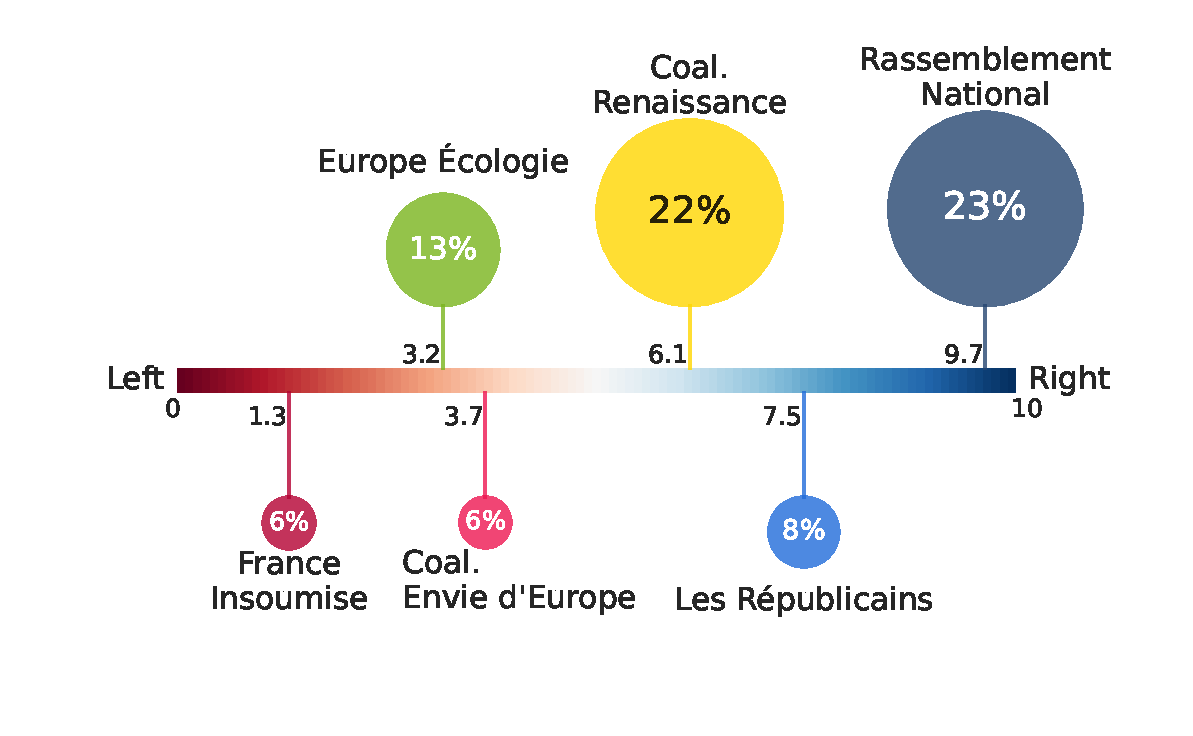
\includegraphics[width=0.8\columnwidth, trim={50pt 55pt 0 0},clip]{images/elections/europe_2019_results_spectrum.pdf}
\label{fig:parlamentary_election_results_spectrum_2019}}\\
\vspace*{-2pt}
\subfloat[2024]{
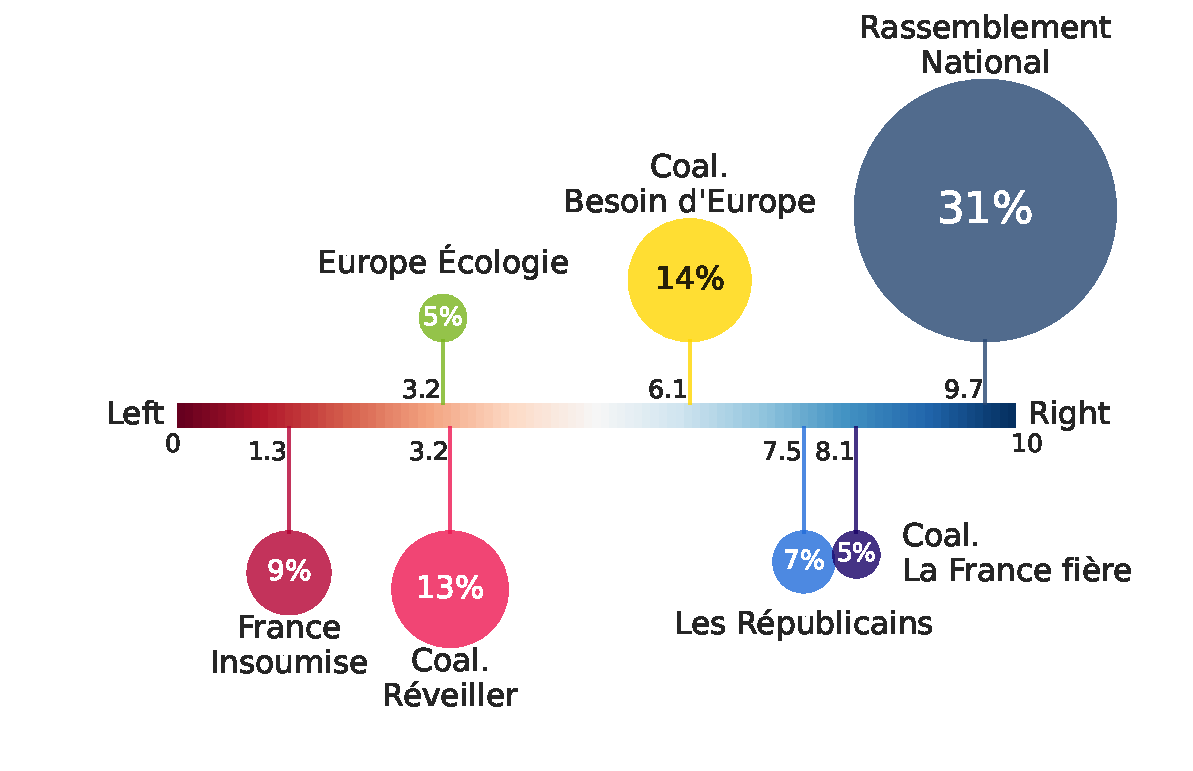
\includegraphics[width=0.8\columnwidth, trim={50pt 30pt 0 0},clip]{images/elections/europe_2024_results_spectrum.pdf}
\label{fig:parlamentary_election_results_spectrum_2024}}
\caption{European Parliamentary election results in France, for parties meeting the $\boldsymbol{5\%}$ vote threshold.
\label{fig:parlamentary_election_results_spectrum_}}
\end{figure}

Six parties cleared the $5\%$ threshold in 2019 and seven in 2024, hence we focus on those and aggregate all remaining parties into a single \textit{others} category to account for $100\%$ of votes.
As also shown in Figure~\ref{fig:parlamentary_election_results_spectrum_}, between the two elections the French political landscape experienced a modest rise in polarization, with growing support for the ideological extremes (\LFI and \RN), the emergence of \REVE and \LFF, and the relative weakening of centrist political forces.
Yet the positioning of all main groups remained fairly stable, which lets us juxtapose our analyses for the two years and carry out a meaningful longitudinal study.
An extended electoral context is provided in Appendix~\ref{app:elections} for readers unfamiliar with the French political landscape.

\section{Data}
\label{sec:data}

Our study hinges upon the integration of multiple data sources:  socioeconomic indicators, election results, communes boundaries, and raw mobile network traffic, which are presented next.
In order to make our results reproducible and to further research, we provide a curated version of the dataset used in this work together with the analysis and modeling code in a public repository\footnote{\href{https://github.com/nds-group/digital-consumption-political-alignment-france}{https://github.com/nds-group/digital-consumption-political-alignment-france}}, see Appendix~\ref{app:data-availability} for a detailed description of the data and code availability.
The raw mobile traffic data remain under \ac{NDA}.

These diverse data types yield high heterogeneity in terms of geographical resolution and scale representation, which requires alignments in the spatiotemporal dimensions as well as in the scale rendering, as discussed in Sections~\ref{sec:data-spatiotemporal} and~\ref{sec:data-scale}, respectively.
Table~\ref{tab:dataset} consolidates the key characteristics of the resulting dataset.

\begin{table}[t]
\centering
\caption{Mobile traffic dataset at a glance. The \ac{MNO} operates two commercial brands, that share a single backbone and are captured as one unsampled dataset. Mobile services are split across thematic categories. Base-station counts denote physical radio cell sites.\label{tab:dataset}}
\small
\setlength{\tabcolsep}{5pt}
\begin{tabular}{l c c}
%\toprule
 & \textbf{2019} & \textbf{2024} \\
\toprule
Mobile lines                & ${\sim}21.8$\,M & ${\sim}22.0$\,M \\
\quad of which low-cost brand & $3.9$\,M & $4.8$\,M \\
Mobile market share         & $31.9\%$ & $31.5\%$ \\
Base stations (nationwide)  & $17{,}567$ & $25{,}894$ \\
\quad in analyzed communes  & $12{,}871$ & $15{,}832$ \\
\midrule
Mobile services (total)     & $22$ & $27$ \\
\quad Social Media          & $6$ & $7$ \\
\quad News                  & $6$ & $6$ \\
\quad Messaging             & $3$ & $5$ \\
\quad Streaming             & $7$ & $9$ \\
\midrule
Urban \& suburban communes  & \multicolumn{2}{c}{$4{,}102$} \\
Coverage (registered voters) & \multicolumn{2}{c}{${\approx}66\%$} \\
Measurement period          & 19--25 May & 2--9 Jun \\
Analysis hours              & \multicolumn{2}{c}{weekday \texttt{20:00}--\texttt{07:00}} \\
\bottomrule
\end{tabular}
\end{table}

\subsection{Sources}
\label{sec:data-sources}

\textbf{Mobile traffic data.} Two measurement campaigns were conducted in 2019 and 2024 in collaboration with a major \ac{MNO} that operates under two commercial brands: its main brand and a low-cost subsidiary, together serving approximately 22~million mobile lines (around 3.9~million of them under the low-cost brand in 2019) and representing a 31.9\% share of the French mobile market in 2019, a share that remained at 31.5\% in 2024~\cite{orange2019,orange2024}.
Both brands share the same backbone infrastructure where the measurement probes are deployed, yielding a \textit{single} dataset that captures the full combined subscriber base with \textit{no sampling}, in contrast to platform-API-based approaches, where even large samples can introduce systematic bias~\cite{di2024sampled}.
The campaigns collected byte counts of mobile service demands at a 1-minute granularity across approximately $17{,}600$ and $25{,}900$ base stations (cell sites) nationwide, and covering 22 and 27 popular mobile services, in 2019 and 2024 respectively, identified by proprietary \ac{DPI} classifiers; the additional services in 2024 (\eg TikTok, Disney+) reflect platforms that gained prominence between the two elections.
For our analysis, we group these services into five categories: \socialmedia, \news, \streaming, \messaging, and \mobile (\ie the union of all tracked services).
Figure~\ref{fig:apps_correlation_with_votes} reports every individual service under its category header for both elections.
Complete technical information about the network architecture, probe deployment, and \ac{DPI} classification is in Appendix~\ref{app:network-data}.
Since our focus is on mobile consumption leading up to the elections, the campaigns measured data from the week preceding polling days in each year, \ie May 19--25 in 2019 and June 2--9 in 2024.

\noindent\textbf{Socioeconomic indicators.} To understand how socioeconomic factors compare to mobile service demand and how much they can explain election outcomes, we incorporate median income, unemployment rate, and population age structure (\ie the number of inhabitants within specific age ranges). These three variables consistently dominate electoral models in France and Western Europe~\cite{bolet2020local,gethin2022brahmin,sipma2020contextual} as discussed in detail in Section~\ref{sec:limitations}.
The indicators were obtained from the National Institute of Statistics and Economic Studies~\cite{soc_pop_income_educ_commune}, which collects and produces data about the French economy and society. 
Figures~\ref{fig:maps-cities-income}--h illustrate the spatial distribution of median income, unemployment ratio, and population density for sample communes in 2019.

\noindent\textbf{Election results.} Electoral results were obtained from the French Ministry of the Interior's open data portal~\cite{elections2019, elections2024}.  
The datasets include the regional code, number of valid, blank, and invalid votes, party names, candidates, and the number of valid votes obtained by each of the competing parties at each polling station.  

\subsection{Spatiotemporal Consolidation}
\label{sec:data-spatiotemporal}

The datasets used in our study exhibit differences in their temporal and spatial granularity.
Resolving these discrepancies is critical to accurately measuring the relationships among the target variables of our study, as discussed next.

\noindent\textbf{Areal consolidation.}
Election results are collected at the \textit{bureau de vote} (\ie polling station) level and subsequently aggregated at commune, department, regional, and national levels.
Similarly, census data and socioeconomic indicators are collected for individual households and aggregated into the different administrative units, the most accurate being the \ac{IRIS}.
For privacy reasons, income and unemployment data are only published for administrative areas with more than $2{,}000$ residents~\cite{soc_pop_income_educ_commune}.
Only a subset of \ac{IRIS} zones meet this threshold, whereas most communes, which represent the second most granular geographical zoning, do.
Therefore, we adopt communes as the spatial unit for our analysis, which lets us ($i$)~access complete data for the vast majority of the French territory unlike what happens with \ac{IRIS} zones, ($ii$)~immediately relate electoral outcomes and socioeconomic indicators that natively employ communes as aggregation levels, and ($iii$)~achieve a suitable trade-off between the preference for higher geographical resolutions and the need for the spatial interpolation of data to be dependable.

\begin{figure}
\centering
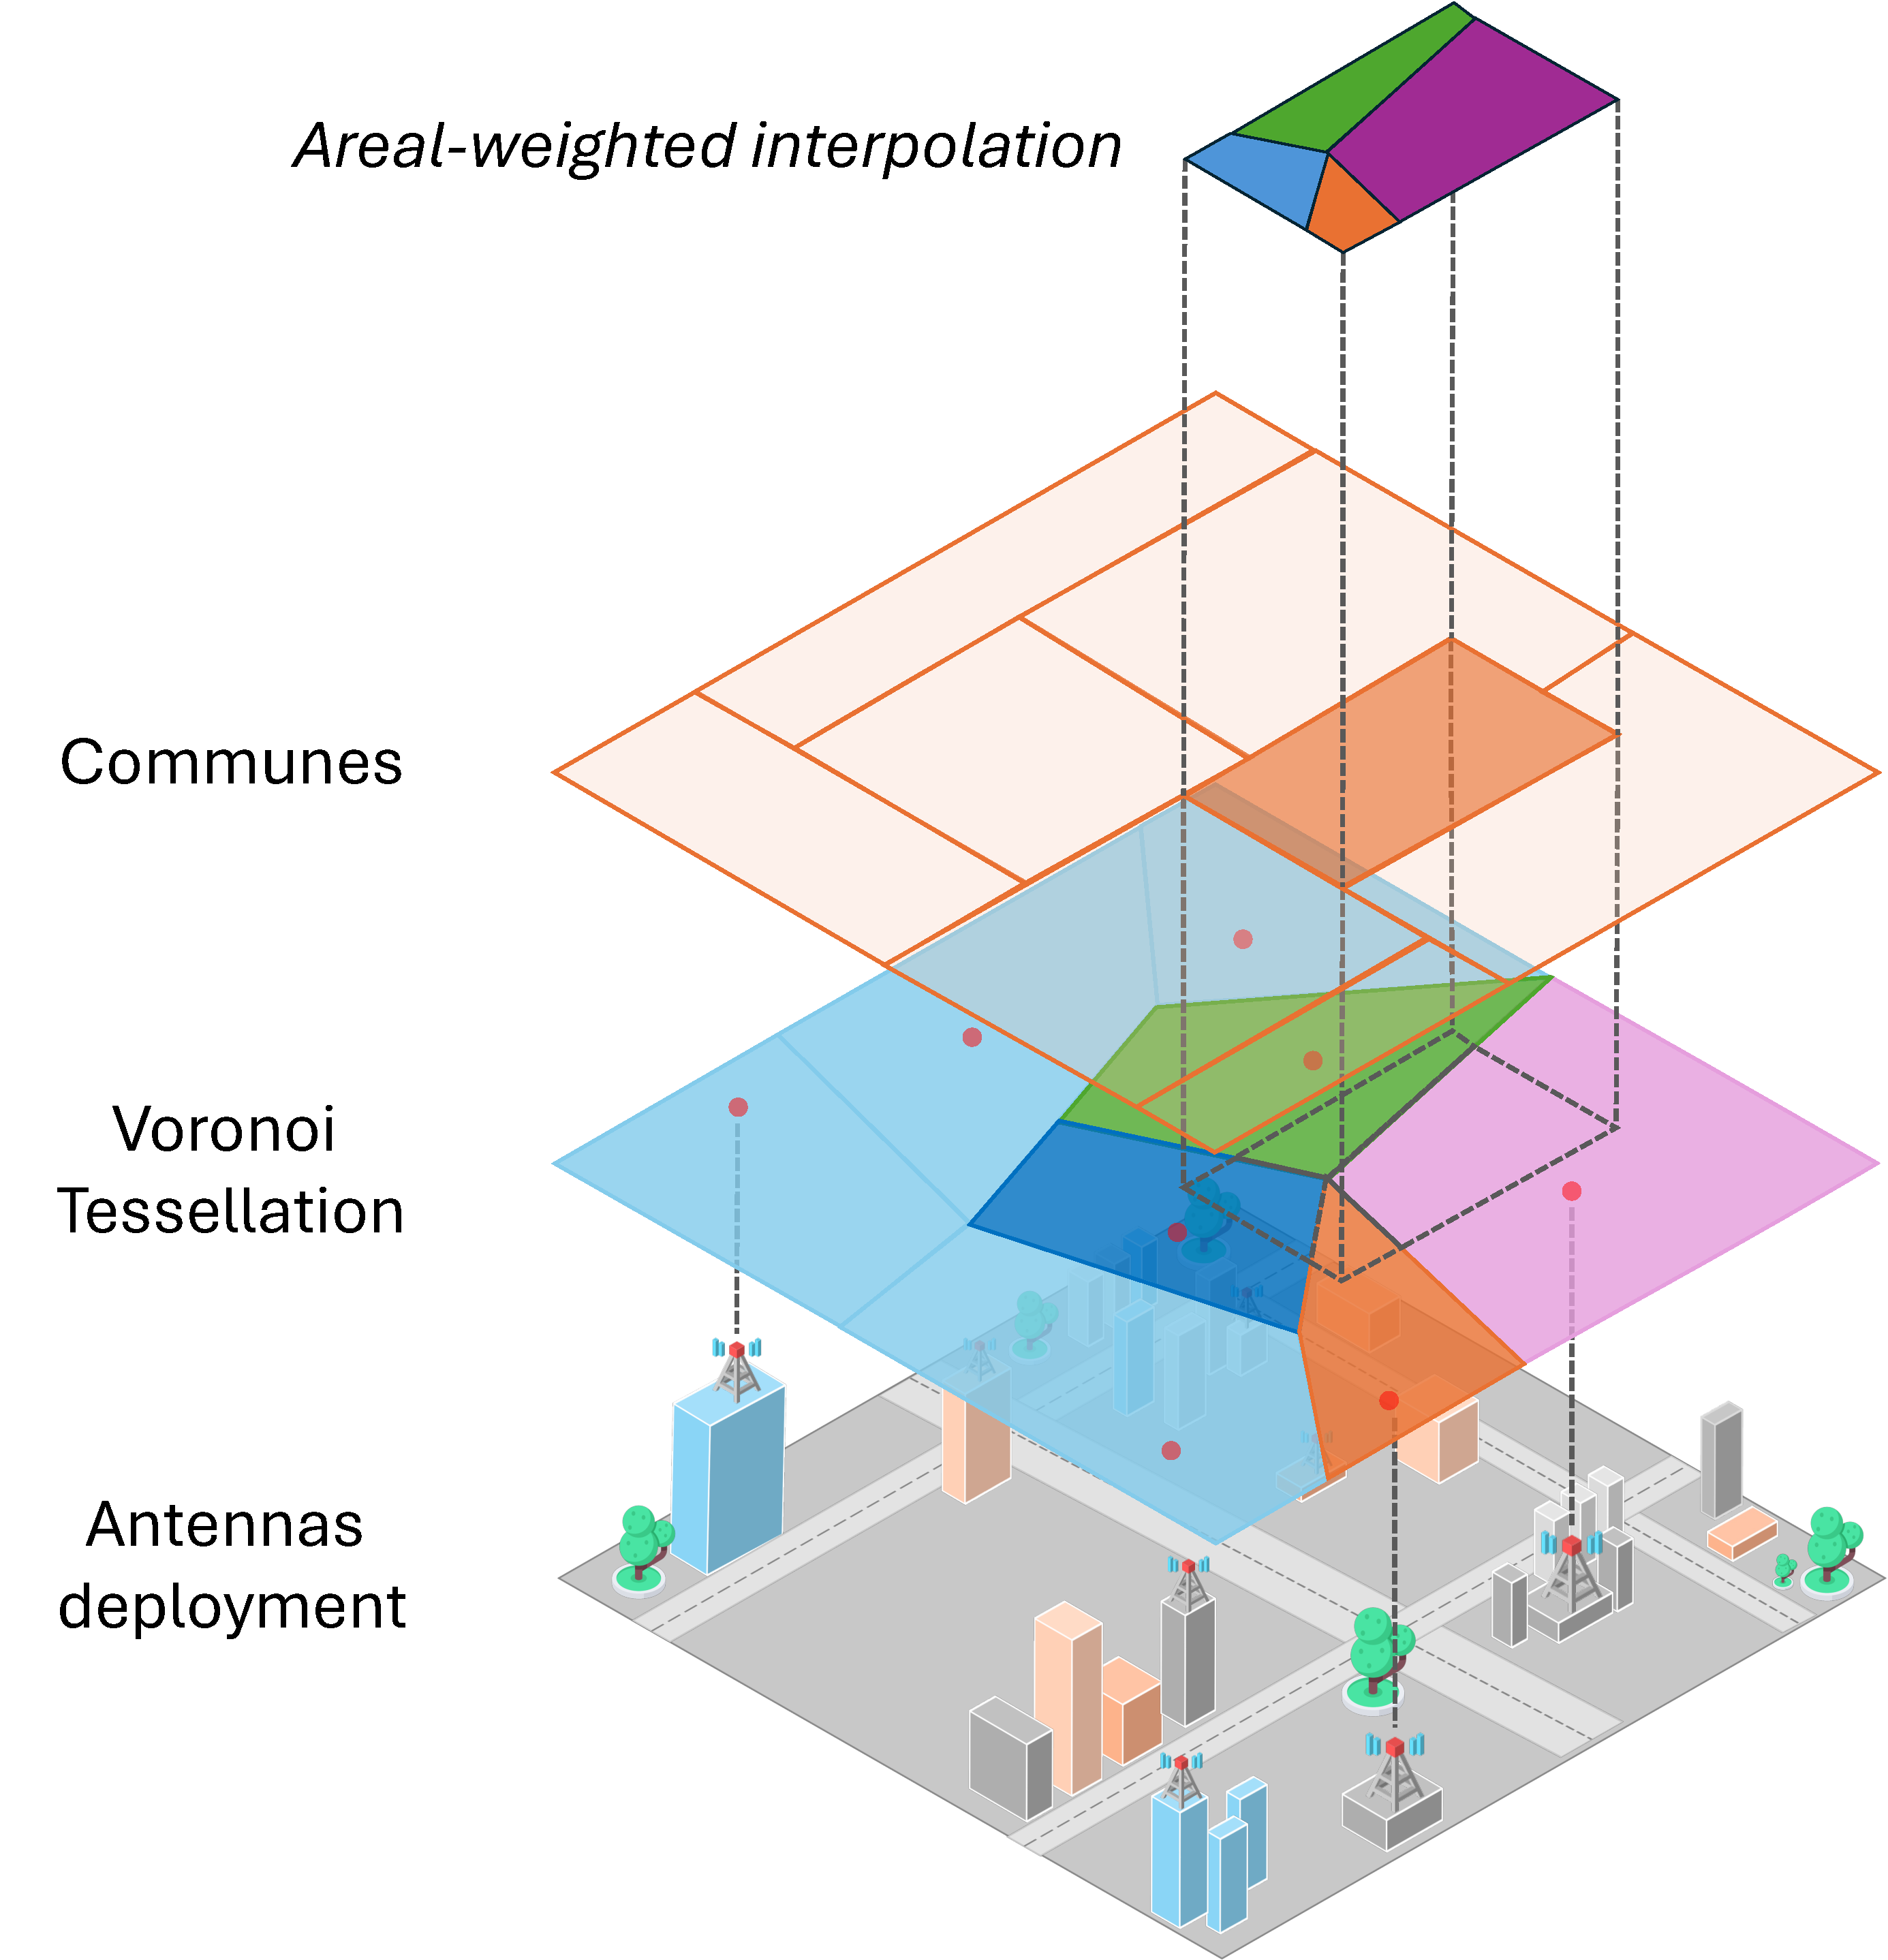
\includegraphics[width=.9\columnwidth]{images/consolidation/voronoi/aereal_interpolation_3d.pdf}
\caption{Illustration of areal-weighted interpolation between Voronoi tesselation and administrative units.
\label{fig:voronoi_interpolation}}
\end{figure}

The last point above relates to the fact that mobile service traffic is geo-referenced at the level of radio access antennas, whose location is known but whose precise coverage area is not disclosed by the \ac{MNO} for confidentiality reasons.
In order to perform a spatial mapping of the mobile service demands recorded at each antenna and align the digital consumption to the other data sources, we rely on the widely adopted practice of relaying on a Voronoi tessellation of space~\cite{voronoi, voronoiboost_secon, 5g_infocom, ucar21news}. This approach is illustrated in Figure~\ref{fig:voronoi_interpolation} and consists in partitioning the target space (whole France%
\footnote{European elections are hold in all French territories, which include several overseas departments like French Guiana or Guadeloupe. Yet our analysis focuses exclusively on so-called \textit{metropolitan} France, as the mobile network data does not cover French territories globally.}
in our case) into Voronoi cells (middle layer in the figure) based on the location of the radio access antennas (lower layer).
Voronoi cells are then spatially intersected with the commune boundaries (top layer) to determine the fraction of each cell overlapping with every commune. Since individual subscriber positions are unavailable, we follow the standard practice in \ac{MNO} spatial analysis of assuming uniform traffic distribution within each Voronoi cell~\cite{ricciato2021estimation,batista2020uncovering,www_20_cellrep,martinez2024deepmend,goel2025predicting}; the overlap fractions serve as weights to proportionally allocate antenna traffic to communes. Cell-level misattribution from this assumption is expected to average out upon aggregation across the multiple cells that overlap each commune.

This areal-weighted interpolation process is reliable when the radio access infrastructure is dense but introduces artifacts in underpopulated regions where antennas are sparsely deployed~\cite{mishra2022digitaldivide}. To avoid the problem, we restrict our analysis to \textit{suburban} and \textit{urban} communes~\cite{commune_urban} where the cellular network is composed of a large number of closely located sites each supporting multiple antennas.
The selected $4{,}102$ communes (identical across both election years) account for approximately $66\%$ of the eligible voting population and
generate over $70\%$ of the mobile demand, which lets us look at more stable mobile service usage patterns and reinforces the statistical dependability of our analysis.
    
\noindent\textbf{Temporal consolidation.}
A temporal mismatch also exists between the mobile traffic data and the socioeconomic indicators.
While mobile service consumption is highly dynamic, census data is relatively static, updated only during periodic survey campaigns.
For this study, we use the 2024 edition of the census dataset~\cite{soc_pop_income_educ_commune}, whose indicators date from 2019 and 2021, the latter being the closest available to the 2024 election at the time of writing.

Mobile service demands measured within a given area over the whole observation period of one week before each election may not exclusively reflect the digital behavior of the local inhabitants, as they include contributions from commuters, temporary visitors, or passers-by.
To improve the alignment between the local voting population and the monitored digital consumption, we restrict our investigation to traffic usage during evening and night hours, \ie when people are most likely to be at home.
Specifically, we consider mobile network traffic generated between \texttt{20:00} and \texttt{07:00} on weekdays only, since previous work~\cite{usage_8} shows that mobile application usage peaks around \texttt{20:00} and remains relatively stable throughout the evening.
We show in Appendix~\ref{app:time-sensitivity} that this choice does not affect the analysis in significant ways in our case and similar results are obtained under different daytime or full-day windowing.


\subsection{Scale Consolidation}
\label{sec:data-scale}

The variables underpinning our analysis are heterogeneous and span very different value ranges. For instance, median income is measured in Euros and can take any value 
% 11730.0, 51720.0
from $11{,}000$ to $52{,}000$, unemployment is expressed as a percentage over the local population, and mobile traffic demands are byte counts per minute. 
This calls for re-scaling the variables so that their correlations are best exposed in the regression.

The issue is especially severe for traffic demands, where the volumes induced by different mobile services vary significantly.
For example, a video streaming application inherently generates much higher traffic than a messaging one, even if they feature similar customer populations and per-user screen time.
As a result, in our mobile traffic dataset, the top $10$ applications in 2024 are responsible for more than $87\%$ of the total mobile demand, and scrolling through TikTok, the single service generating the most data, causes over $10^4\times$ higher traffic than browsing online news, which may however be a more important service to explain political alignment.
To ensure comparability across mobile services, we employ a modified version of the \ac{RCA} index~\cite{rca}, originally developed in economics to measure a country’s relative advantage or disadvantage in the production of specific goods or services based on trade flows. 
The \ac{RCA}, and its application to network traffic characterization, has also been established in the literature~\cite{mishra2022digitaldivide,ucar21news,goel2025predicting}.
More precisely, we reinterpret this metric to capture a \textit{service advantage} across communes, \ie to expose communes where the usage of a service is substantially different than the national average.

Formally, for each commune and mobile service, we first aggregate the total byte counts (accounting for both uplink and downlink traffic) across all evening and night hours of the reference week before each election. Next, we normalize the obtained values by the number of local inhabitants to obtain the per-capita consumption $T_{ij}$ of a given service $j$ in commune $i$.
The associated \ac{RCA} index is then computed as:
\begin{equation}
\text{RCA}_{ij} = \frac{T_{ij} / \sum_k T_{ik}}{\sum_h T_{hj} / \sum_h \sum_k T_{hk}},
\label{eq:rca_traffic}
\end{equation}
where 
$\sum_k T_{ik}$ is the total traffic per inhabitant in commune $i$, aggregated over all services,
$\sum_h T_{hj}$ is the mean traffic per inhabitant for service $j$ observed across all communes,
and $\sum_h \sum_k T_{hk}$ is the total traffic generated by the average inhabitant of France.
Therefore, the enumerator captures the mean prevalence of a specific service $j$ within the total mobile demand in a commune $i$, whereas the denominator represents the same metric but at a national scale, \ie when aggregating digital usage data from all communes.


A service $j$ is said to have a \textit{comparative advantage} in commune $i$ if $\text{RCA}_{ij} > 1$, implying a higher-than-ordinary usage of service $j$ in that commune; conversely if $\text{RCA}_{ij} < 1$ suggests that service $j$ presents a \textit{comparative disadvantage}, \ie a reduced adoption in commune $i$ with respect to the national average.
However, the \ac{RCA} may still yield extreme values due to large variations in service usage across locations, as well as non-comparable trends for advantage (characterized by an unbounded linear increase as one moves away from the origin) and disadvantage (featuring non-linear harmonic decline bounded by $-1$) cases.
To mitigate these effects, we use a normalized, symmetric version of \ac{RCA}, named \ac{SRCA}:
\begin{equation}
\text{sRCA}_{ij} = \frac{\text{RCA}_{ij} - 1}{\text{RCA}_{ij} + 1},
\end{equation}
which rescales the $\text{RCA}$ values to the range $(-1, 1)$, ensuring symmetry around zero and reducing the influence of outliers.
The interpretation remains the same with positive values indicating \textit{comparative advantage} while negative values indicate a \textit{comparative disadvantage}.
Overall, these transformations enable a fair comparison of mobile service demand across applications, reducing distortions from intrinsic differences in per-application content type and data volumes.
Appendix~\ref{app:srca} provides a visual walkthrough of the raw-to-\ac{SRCA} transformation for representative services.

Finally, all mobile service and socioeconomic variables are standardized via a division by their sample standard deviation.
This transformation brings all variables onto a comparable numerical scale and prevents those with larger magnitudes from dominating the regression in Section~\ref{sec:explain-model}.

\begin{figure*}[t!]
\raggedleft
\subfloat{
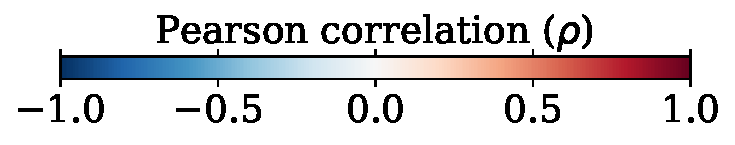
\includegraphics[height=.05\textwidth]{images/correlation_matrix/colorbar.pdf}}

\centering
%\subfloat[2019]{
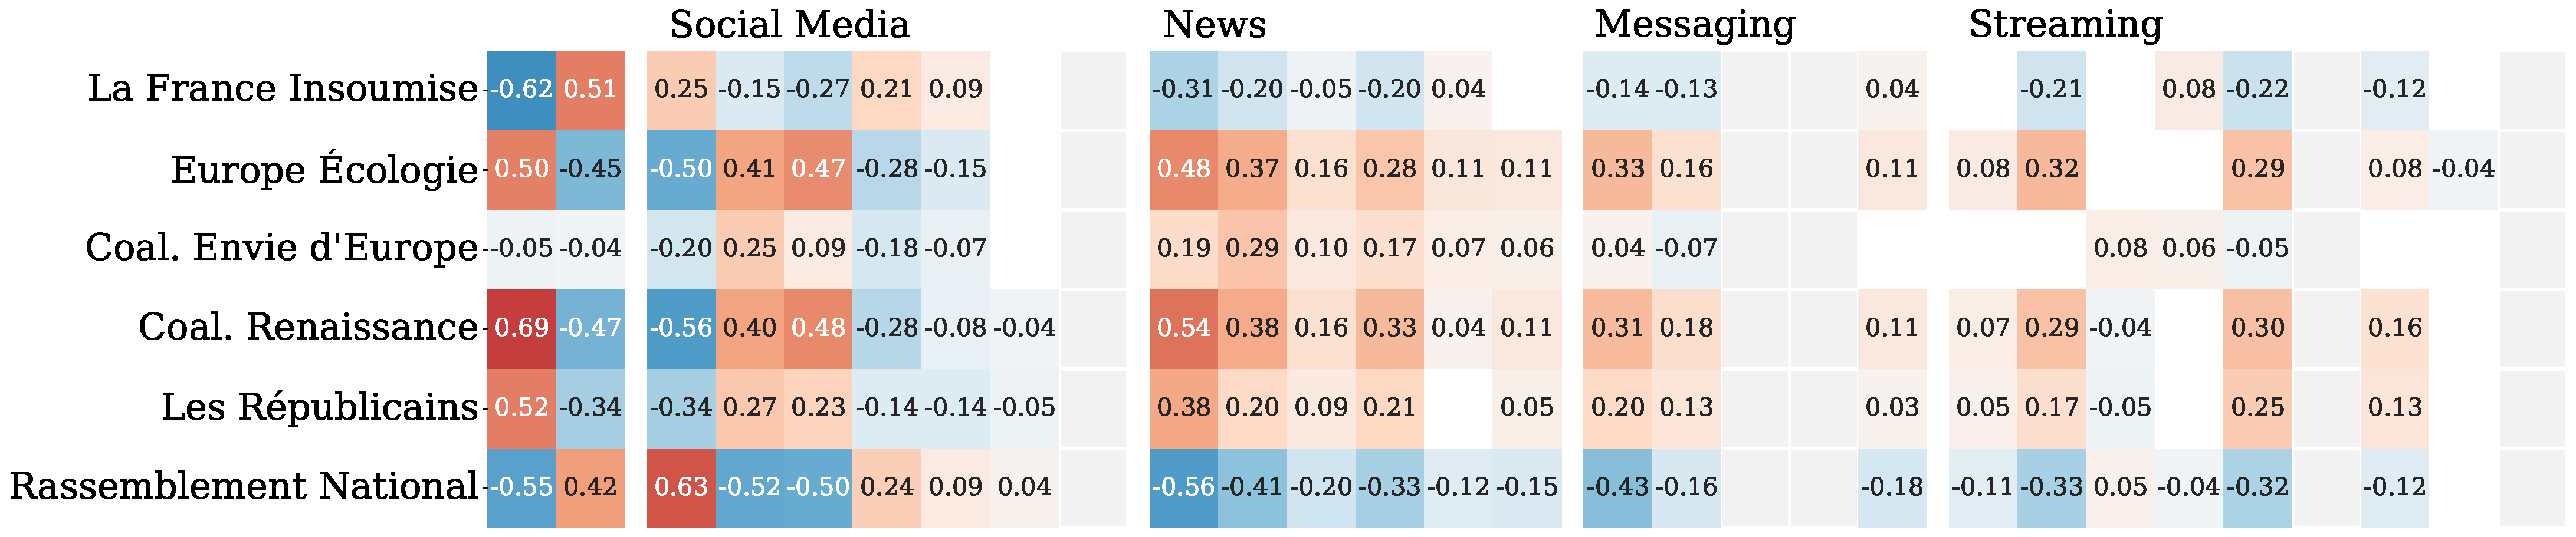
\includegraphics[width=.98\linewidth]{images/correlation_matrix/europe_2019_correlation_matrix_Urban and Suburban Communes_horizontal.pdf}\\
\vspace*{4pt}
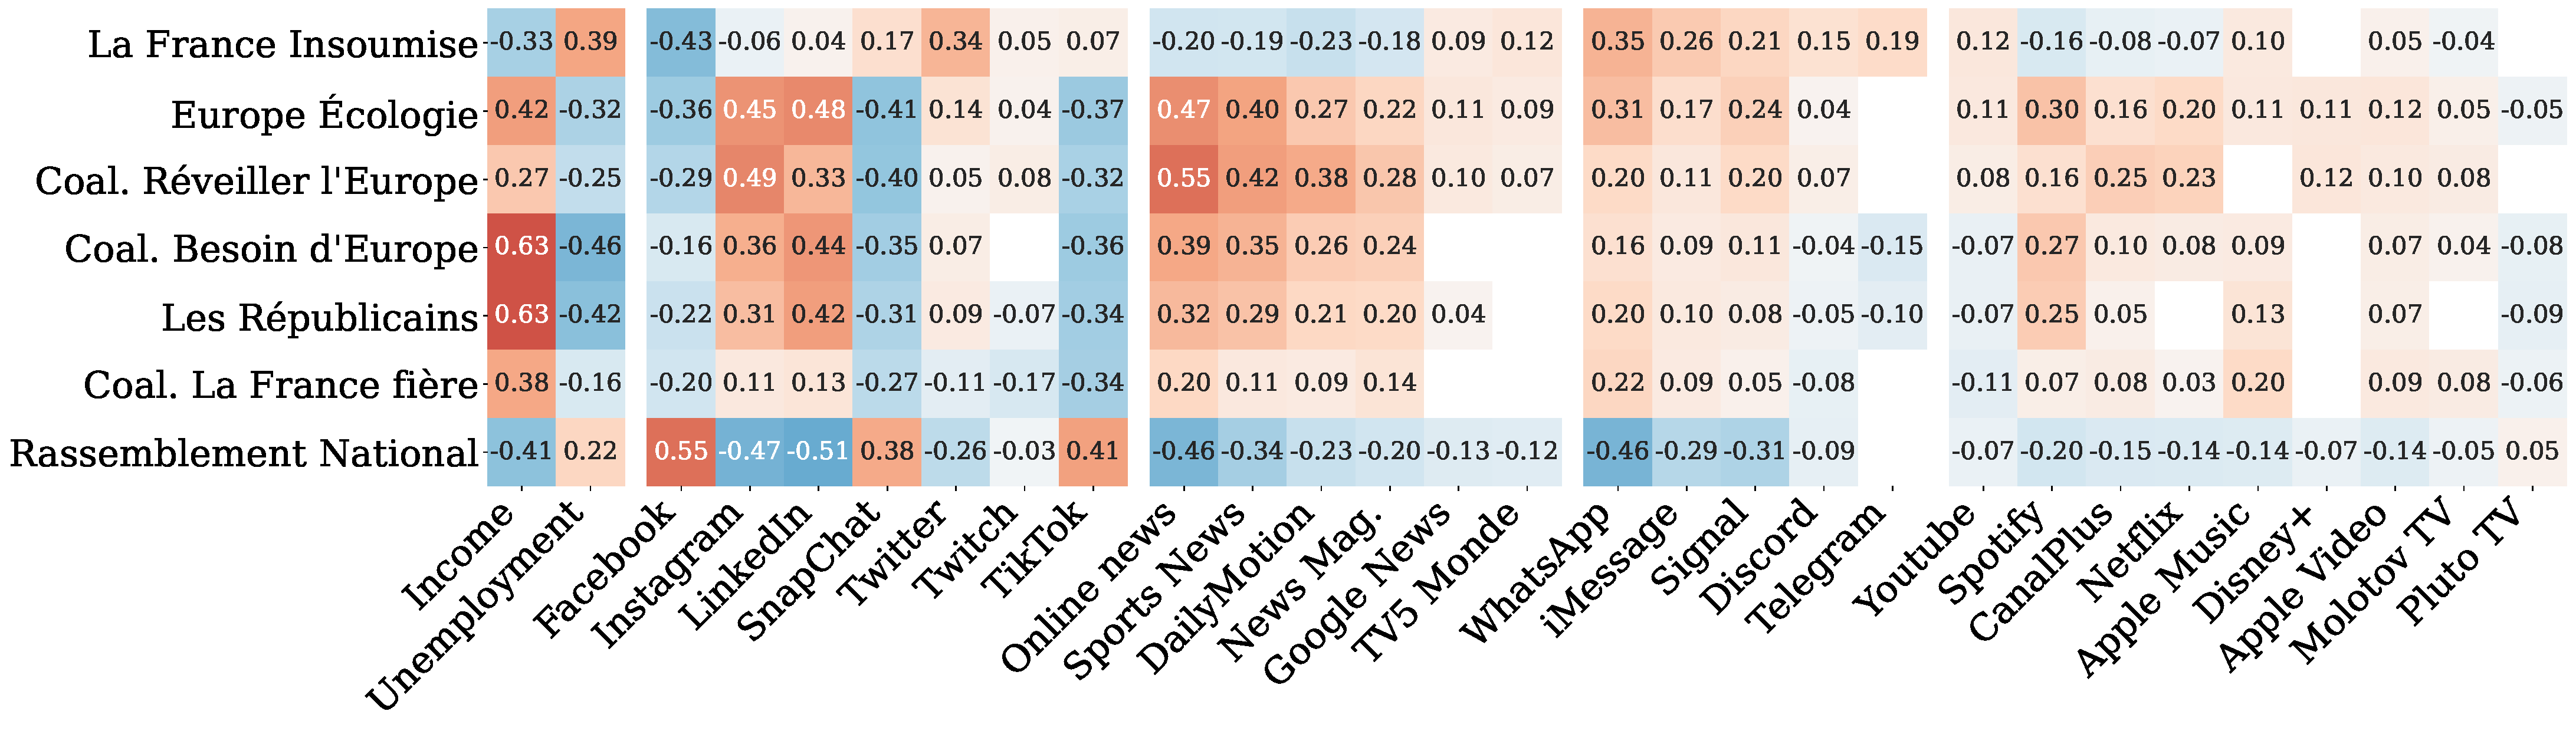
\includegraphics[width=.98\linewidth]{images/correlation_matrix/europe_2024_correlation_matrix_Urban and Suburban Communes_horizontal.pdf}
\vspace{-8pt}
\caption{Correlation between variables and political parties’ vote shares in 2019 (top) and 2024 (bottom). Empty cells denote non-significant correlations ($\boldsymbol{p}$-value~$\boldsymbol{>0.05}$), grey cells indicate missing services in 2019. 
\label{fig:apps_correlation_with_votes}}
\end{figure*}


\section{Explaining Election Results}
\label{sec:explain}

We introduce a two-step methodology to assess the extent to which mobile service consumption is associated with election outcomes, relative to traditional socioeconomic indicators.
First, in Section~\ref{sec:explain-correlation} we analyze the pairwise correlation between vote shares and both individual socioeconomic indicators and mobile service usages.
Second, in Section~\ref{sec:explain-model} we employ a regression model adapted to our target problem and to guarantee interpretability.

\subsection{Correlation Analysis}
\label{sec:explain-correlation}

We start by carrying out an exploratory analysis of the correlations between vote and individual variables in both the traditional socioeconomic status space as well as in the digital consumption domain.
%
Figure~\ref{fig:apps_correlation_with_votes} summarizes the Pearson's coefficient $\rho$ of pairwise linear correlations of each target variable, \ie the share of votes obtained by each political party across communes in France (as rows), to every input variable, \ie individual socioeconomic indicators or mobile application demands (as columns).

Overall, the initial correlation analysis shows promise, with significant concurrence in the values of specific digital usage input and target vote variables that lead to $\rho$ as high as $0.63$, for the case of Facebook and \RN. More generally, applications such as the same Facebook, Instagram, LinkedIn, Snapchat, or online news (which gathers traffic generated by access to the websites of newspapers) show explanatory capabilities that are on par with those of customary socioeconomic predictors like income or the level of unemployment. Importantly, correlations appears largely stable across the 2019 and 2024 elections, corroborating the solidity of the observed relationships.

Delving into the sign and values of $\rho$ reveals how a higher consumption of some mobile services is associated to a stronger \textit{political polarization}, \ie a tendency to vote for far Left or far Right parties: this is the case of Facebook or Snapchat. The opposite also happens, with other applications signaling a local preference for more moderate parties: examples include Instagram or online news.
Yet, we observe the same effects in socioeconomic indicators, with, \eg unemployment favoring polarization and income more centrist parties.
Therefore, a legitimate doubt is whether the effects we observe for the mobile service consumption variables are rightful bonds to political alignment or just proxies for the socioeconomic ones, \eg because more affluent individuals also use LinkedIn or read online news more often.

The key question is whether digital usages \textit{add} predictive power beyond conventional socioeconomic indicators.
%
Simple pairwise regression cannot answer that question, which instead requires multivariate analyses that compare the goodness of fit of models using diverse combination of input variables. However, straightforward multivariate models that use subsets of all input socioeconomic and mobile demand variables to predict the vote share of a single party are not suitable for our analysis either.
The reason is that election outcomes, represented as party vote shares, are compositional in nature, since the proportions across parties are non-negative and sum to a fixed $100\%$ total.
In a pure two-party system, this constraint can be ignored: modeling one party’s vote share automatically determines the other~\cite{hanretty2021forecasting}.
However, in multiparty elections, neglecting this compositional structure can lead to inconsistent or logically impossible predictions where the total vote share exceeds $100\%$.
Properly regressing political alignment therefore requires a dedicated methodology, which we develop next.

\subsection{Regressing Vote in Multiparty Elections}
\label{sec:explain-model}

Our strategy to explaining political alignment in multiparty elections hinges upon Dirichlet Regression~\cite{hanretty2021forecasting, maier2014dirichletreg} as a suitable modeling framework for compositional data.
This approach estimates the parameters of a continuous multivariate Dirichlet distribution, ensuring that the predicted vote shares across all parties sum to $100\%$.
Formally, the Dirichlet distribution is defined as:
\begin{equation}
\mathcal{D}(\mathcal{V}, \alpha) = \frac{1}{\mathcal{B}(\alpha)} \prod_{l=1}^{N} v_{l}^{(\alpha_{l} -1)},
\label{eq:dirichlet_distribution}
\end{equation}
where $\mathcal{B}(\alpha)$ is the multivariate Beta function, and $\alpha$ is a \textit{concentration vector} of length $N$ that determines the location of the center of mass of the distribution across its $N$ dimensions.
In our case, each dimension corresponds to a political party, and $v_l$ represents the vote share of party $l$.
Our goal is to estimate the components $\alpha_p$ of the vector $\alpha$ that best fit the observed vote share distribution in the $n$-dimensional space.

\begin{figure}
\centering
\subfloat{
%\setcounter{subfigure}{0}
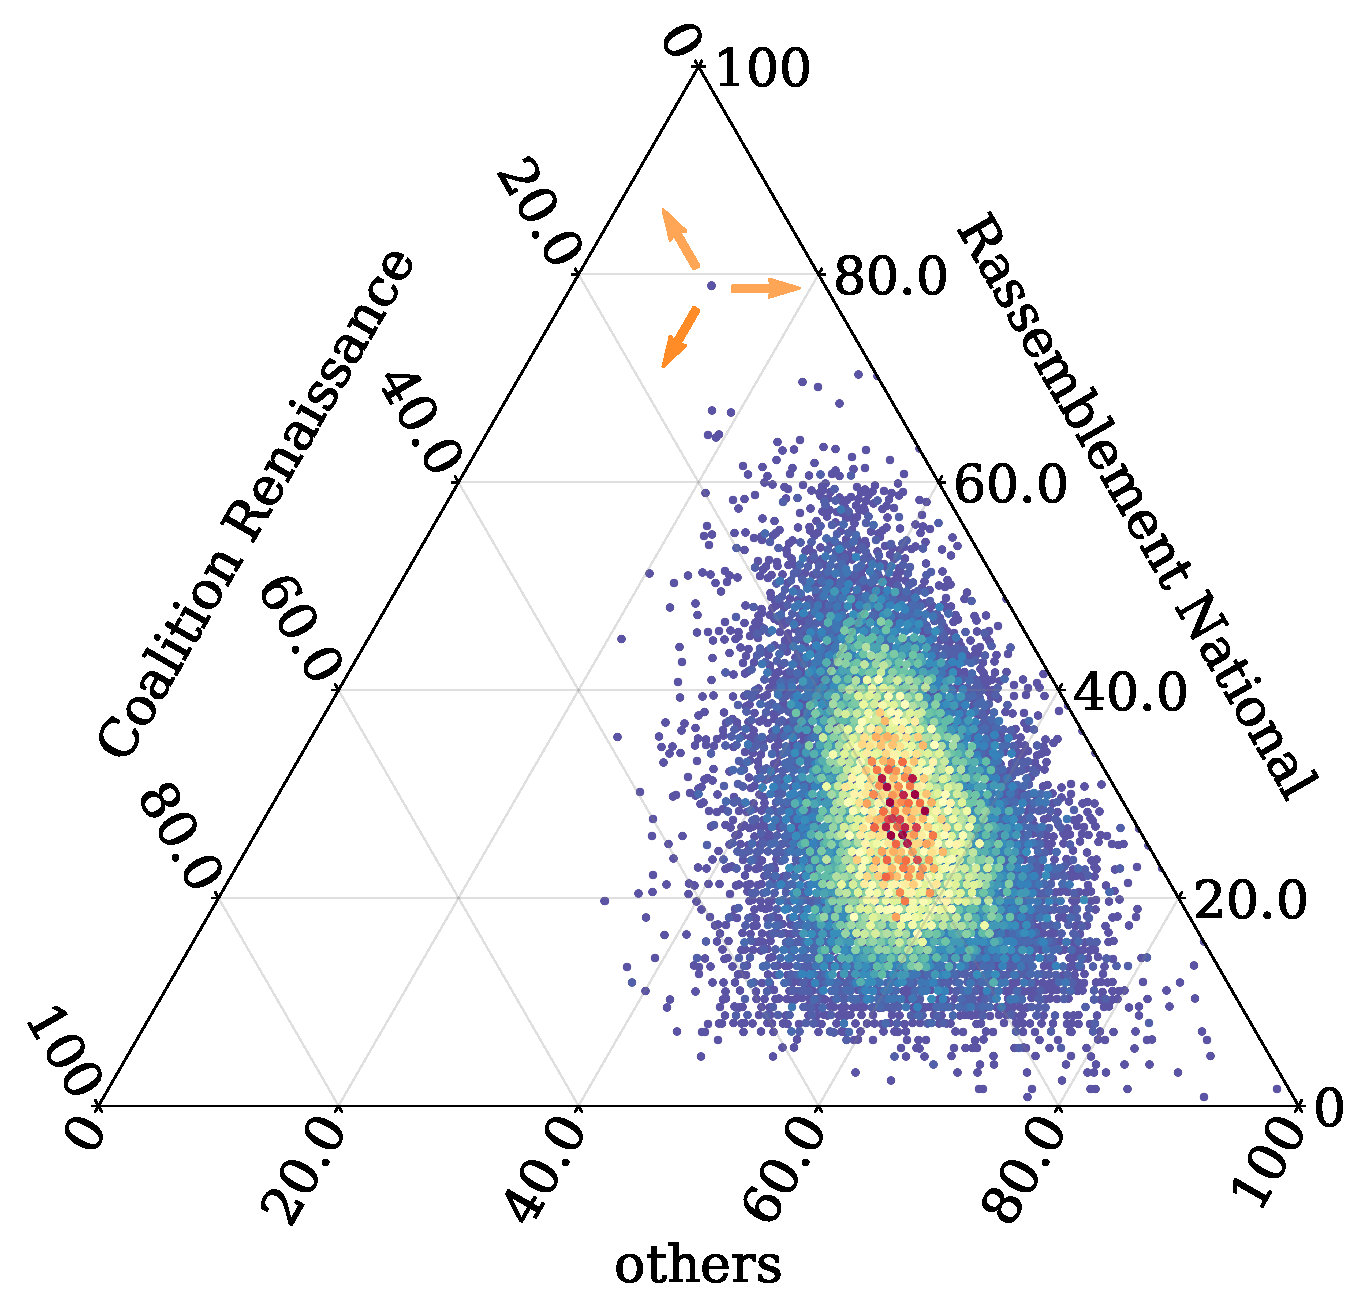
\includegraphics[width=.6\columnwidth]{images/dirichlet_distribution/ternary_3d.pdf}}
\hspace*{4pt}
\raisebox{40pt}{%
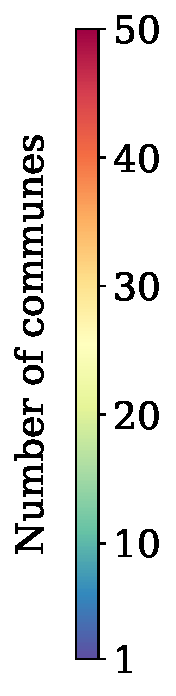
\includegraphics[width=.11\columnwidth]{images/dirichlet_distribution/ternary_3d_colorbar_vertical.pdf}}
\vspace{-8pt}
\caption{Dirichlet distribution as a ternary plot for a simplified case where votes in the 2019 elections are shared among three groups, \ie \RN, \RENA, and any other party.
\label{fig:dirichlet_density}}
\end{figure}

Figure~\ref{fig:dirichlet_density} shows a simplified illustration of the empirical distribution for the 2019 election results using a ternary plot. 
Two sides are associated with the two main parties, \RN and \RENA, while all other parties are grouped under a single \textit{others} category.
For this example, the $\alpha$ vector that best fits the distribution is $\alpha=(2.24, 1.89, 2.88)$, meaning that the center of mass of the distribution is concentrated primarily on the third dimension (others), followed by the first dimension (\RN), with lower probability on the second dimension (\RENA).
The objective of the Dirichlet regression is then to model the $\alpha$ vector based on the socioeconomic and digital usage indicators for each commune.

\noindent\textbf{Coefficients.}
We fit the model in~\eqref{eq:dirichlet_distribution} via maximum likelihood estimation \cite{maier2014dirichletreg}. Here, each $\alpha_p$ component is expressed as a function of a set of predictor variables, which can take many forms; for the sake of \textit{interpretability} of the fitted model, we restrict our analysis to linear relationships, formally:
\begin{equation}
\alpha_p = \sum_q \beta_q x_q + \gamma_p,
\label{eq:regression_coefficients}
\end{equation}
where $\beta_q$ are the regression coefficients, $x_q$ represent the predictor variables, such as mobile service consumption and socioeconomic indicators, and $\gamma_p$ is the intercept.
This formulation enables a straightforward interpretation of coefficients, analogous to that of a standard linear regression.


\begin{table}
\centering 
%\scriptsize
\caption{Sets of variables used for Dirichlet regression.\label{tab:sets_predictor_variables_election}}
\resizebox{.49\textwidth}{!} { 
\begin{tabular}{p{2in} | c | c | c | c | c | c | c | c | c | c }
\multicolumn{1}{l}{\textbf{Sample variables}} & 
\multicolumn{1}{l}{\makebox[0pt][l]{\hspace{-5pt}\rotatebox{30}{\population}}} & 
\multicolumn{1}{l}{\makebox[0pt][l]{\hspace{-5pt}\rotatebox{30}{\unemployment}}} & 
\multicolumn{1}{l}{\makebox[0pt][l]{\hspace{-5pt}\rotatebox{30}{\income}}} & 
\multicolumn{1}{l}{\makebox[0pt][l]{\hspace{-5pt}\rotatebox{30}{\socioeconomic}}} & 
\multicolumn{1}{l}{\makebox[0pt][l]{\hspace{-5pt}\rotatebox{30}{\streaming}}} & 
\multicolumn{1}{l}{\makebox[0pt][l]{\hspace{-5pt}\rotatebox{30}{\news}}} & 
\multicolumn{1}{l}{\makebox[0pt][l]{\hspace{-5pt}\rotatebox{30}{\messaging}}} & 
\multicolumn{1}{l}{\makebox[0pt][l]{\hspace{-5pt}\rotatebox{30}{\socialmedia}}} & 
\multicolumn{1}{l}{\makebox[0pt][l]{\hspace{-5pt}\rotatebox{30}{\mobile}}} & 
\multicolumn{1}{l}{\makebox[0pt][l]{\hspace{-5pt}\rotatebox{30}{\all}}} \\[.2em]
\cline{1-11}
Fraction of population in five age intervals, breaking at 15, 30, 45, 60 & $\checkmark$ &  &  & $\checkmark$ &  &  &  &  &  &$\checkmark$ \\
\cellcolor{blue!15} Fraction of unemployed inhabitants & \cellcolor{blue!15} & \cellcolor{blue!15} $\checkmark$ & \cellcolor{blue!15} & \cellcolor{blue!15} $\checkmark$ & \cellcolor{blue!15} & \cellcolor{blue!15} & \cellcolor{blue!15} & \cellcolor{blue!15} & \cellcolor{blue!15} & \cellcolor{blue!15} $\checkmark$ \\
Median household income &  &  & $\checkmark$ & $\checkmark$ &  &  &  &  &  & $\checkmark$ \\
\cline{1-11}
\cellcolor{blue!15} YouTube, Spotify, Netflix, Disney+ & \cellcolor{blue!15} & \cellcolor{blue!15} & \cellcolor{blue!15} & \cellcolor{blue!15} & \cellcolor{blue!15} $\checkmark$ & \cellcolor{blue!15} & \cellcolor{blue!15} & \cellcolor{blue!15} & \cellcolor{blue!15} $\checkmark$ & \cellcolor{blue!15} $\checkmark$ \\
Online news, DailyMotion &  &  &  &  &  & $\checkmark$ &  &  & $\checkmark$ & $\checkmark$ \\
\cellcolor{blue!15} WhatsApp, Signal, Telegram & \cellcolor{blue!15} & \cellcolor{blue!15} & \cellcolor{blue!15} & \cellcolor{blue!15} & \cellcolor{blue!15} & \cellcolor{blue!15} & \cellcolor{blue!15} $\checkmark$ & \cellcolor{blue!15} & \cellcolor{blue!15} $\checkmark$ & \cellcolor{blue!15} $\checkmark$ \\
Facebook, Instagram, TikTok &  &  &  &  &  &  &  &  $\checkmark$ & $\checkmark$ & $\checkmark$ 
\end{tabular}}
\end{table}

\noindent\textbf{Predictors.}
To assess the explanatory power of socioeconomic indicators and mobile service demand, we evaluate $10$ different sets of predictor variables.
These sets range from individual variables to all socioeconomic and mobile service variables combined (Table~\ref{tab:sets_predictor_variables_election}).
This lets us quantify each group's contribution to model performance and how much mobile service usage complements traditional socioeconomic factors in explaining voting behavior.

\noindent\textbf{Goodness of fit.}
Standard $R^2$ measures are not directly applicable to maximum-likelihood models such as Dirichlet regression. We therefore compute a predictive $R^2$, defined as the coefficient of determination ($1 - SS_{res}/SS_{tot}$) between observed and predicted vote shares, which quantifies the proportion of variance in voting outcomes explained by the model.
Since this metric increases monotonically as more predictors are added, we apply the Adjusted $R^2$ (\adjrsquare hereinafter) correction~\cite{james2013introduction} to enable a fair comparison across models with different numbers of variables. Specifically, this adjustment penalizes the inclusion of additional predictors and prevents overestimating the model’s explanatory power.
We note that the OLS \adjrsquare formula is not formally derived for maximum-likelihood models; we apply it here as a practical complexity penalty, and complement it with the \ac{AIC}, the \ac{BIC}, and log-likelihood in Appendix~\ref{app:aic-bic}.
Formally, our Dirichlet goodness-of-fit metric is:
\begin{equation}
\text{Adj.}~R^2 = 1 - \frac{(1-R^2)(n-1)}{n-p-1},
\label{eq:political_election_explanation_adj_r2}
\end{equation}
where $R^2$ is the predictive $R^2$, $n$ is the number of observations, and $p$ is the number of explanatory variables.
Higher \adjrsquare indicates better model fit, % given the number of parameters,
with values near $1$ indicating the model captures most of the variation in voting patterns.

\noindent\textbf{Multicollinearity.}
Considering the large set of variables employed, we control for multicollinearity, quantified using the \ac{VIF}~\cite{james2013introduction} defined as:
\begin{equation}
\text{VIF}(x_m) = \frac{1}{1 - {R^2}(x_m)},
\end{equation}
where ${R^2}(x_m)$ is obtained by regressing variable $x_m$ on all other predictors.
High \ac{VIF} values indicate strong collinearity; values above $10$ are typically considered problematic~\cite{weisberg2005applied}.
The mean \ac{VIF} for 2019 is $1.68$, with a maximum of $3.53$ for Facebook, while in 2024, the mean is $2.20$, and the maximum is $5.50$ for TV5MONDE.
All values remain below the reference threshold, suggesting that although some mobile service variables are moderately correlated, they can each contribute distinct information.
Based on this outcome, we retain all variables in the subsequent regression analysis.

\section{Results}
\label{sec:results}

In this section, we evaluate how well the different sets of predictors explain political alignment, with a focus on the contribution of mobile service consumption indicators. We present goodness-of-fit results in Section~\ref{sec:results-gof}, visuals about the spatial quality of the model predictions in Section~\ref{sec:results-spatial}, and a discussion of the regression coefficients in Section~\ref{sec:results-coefficient}.

\subsection{Goodness of Fit}
\label{sec:results-gof}

\begin{figure*}[t]
% \centering
\subfloat[2019]{
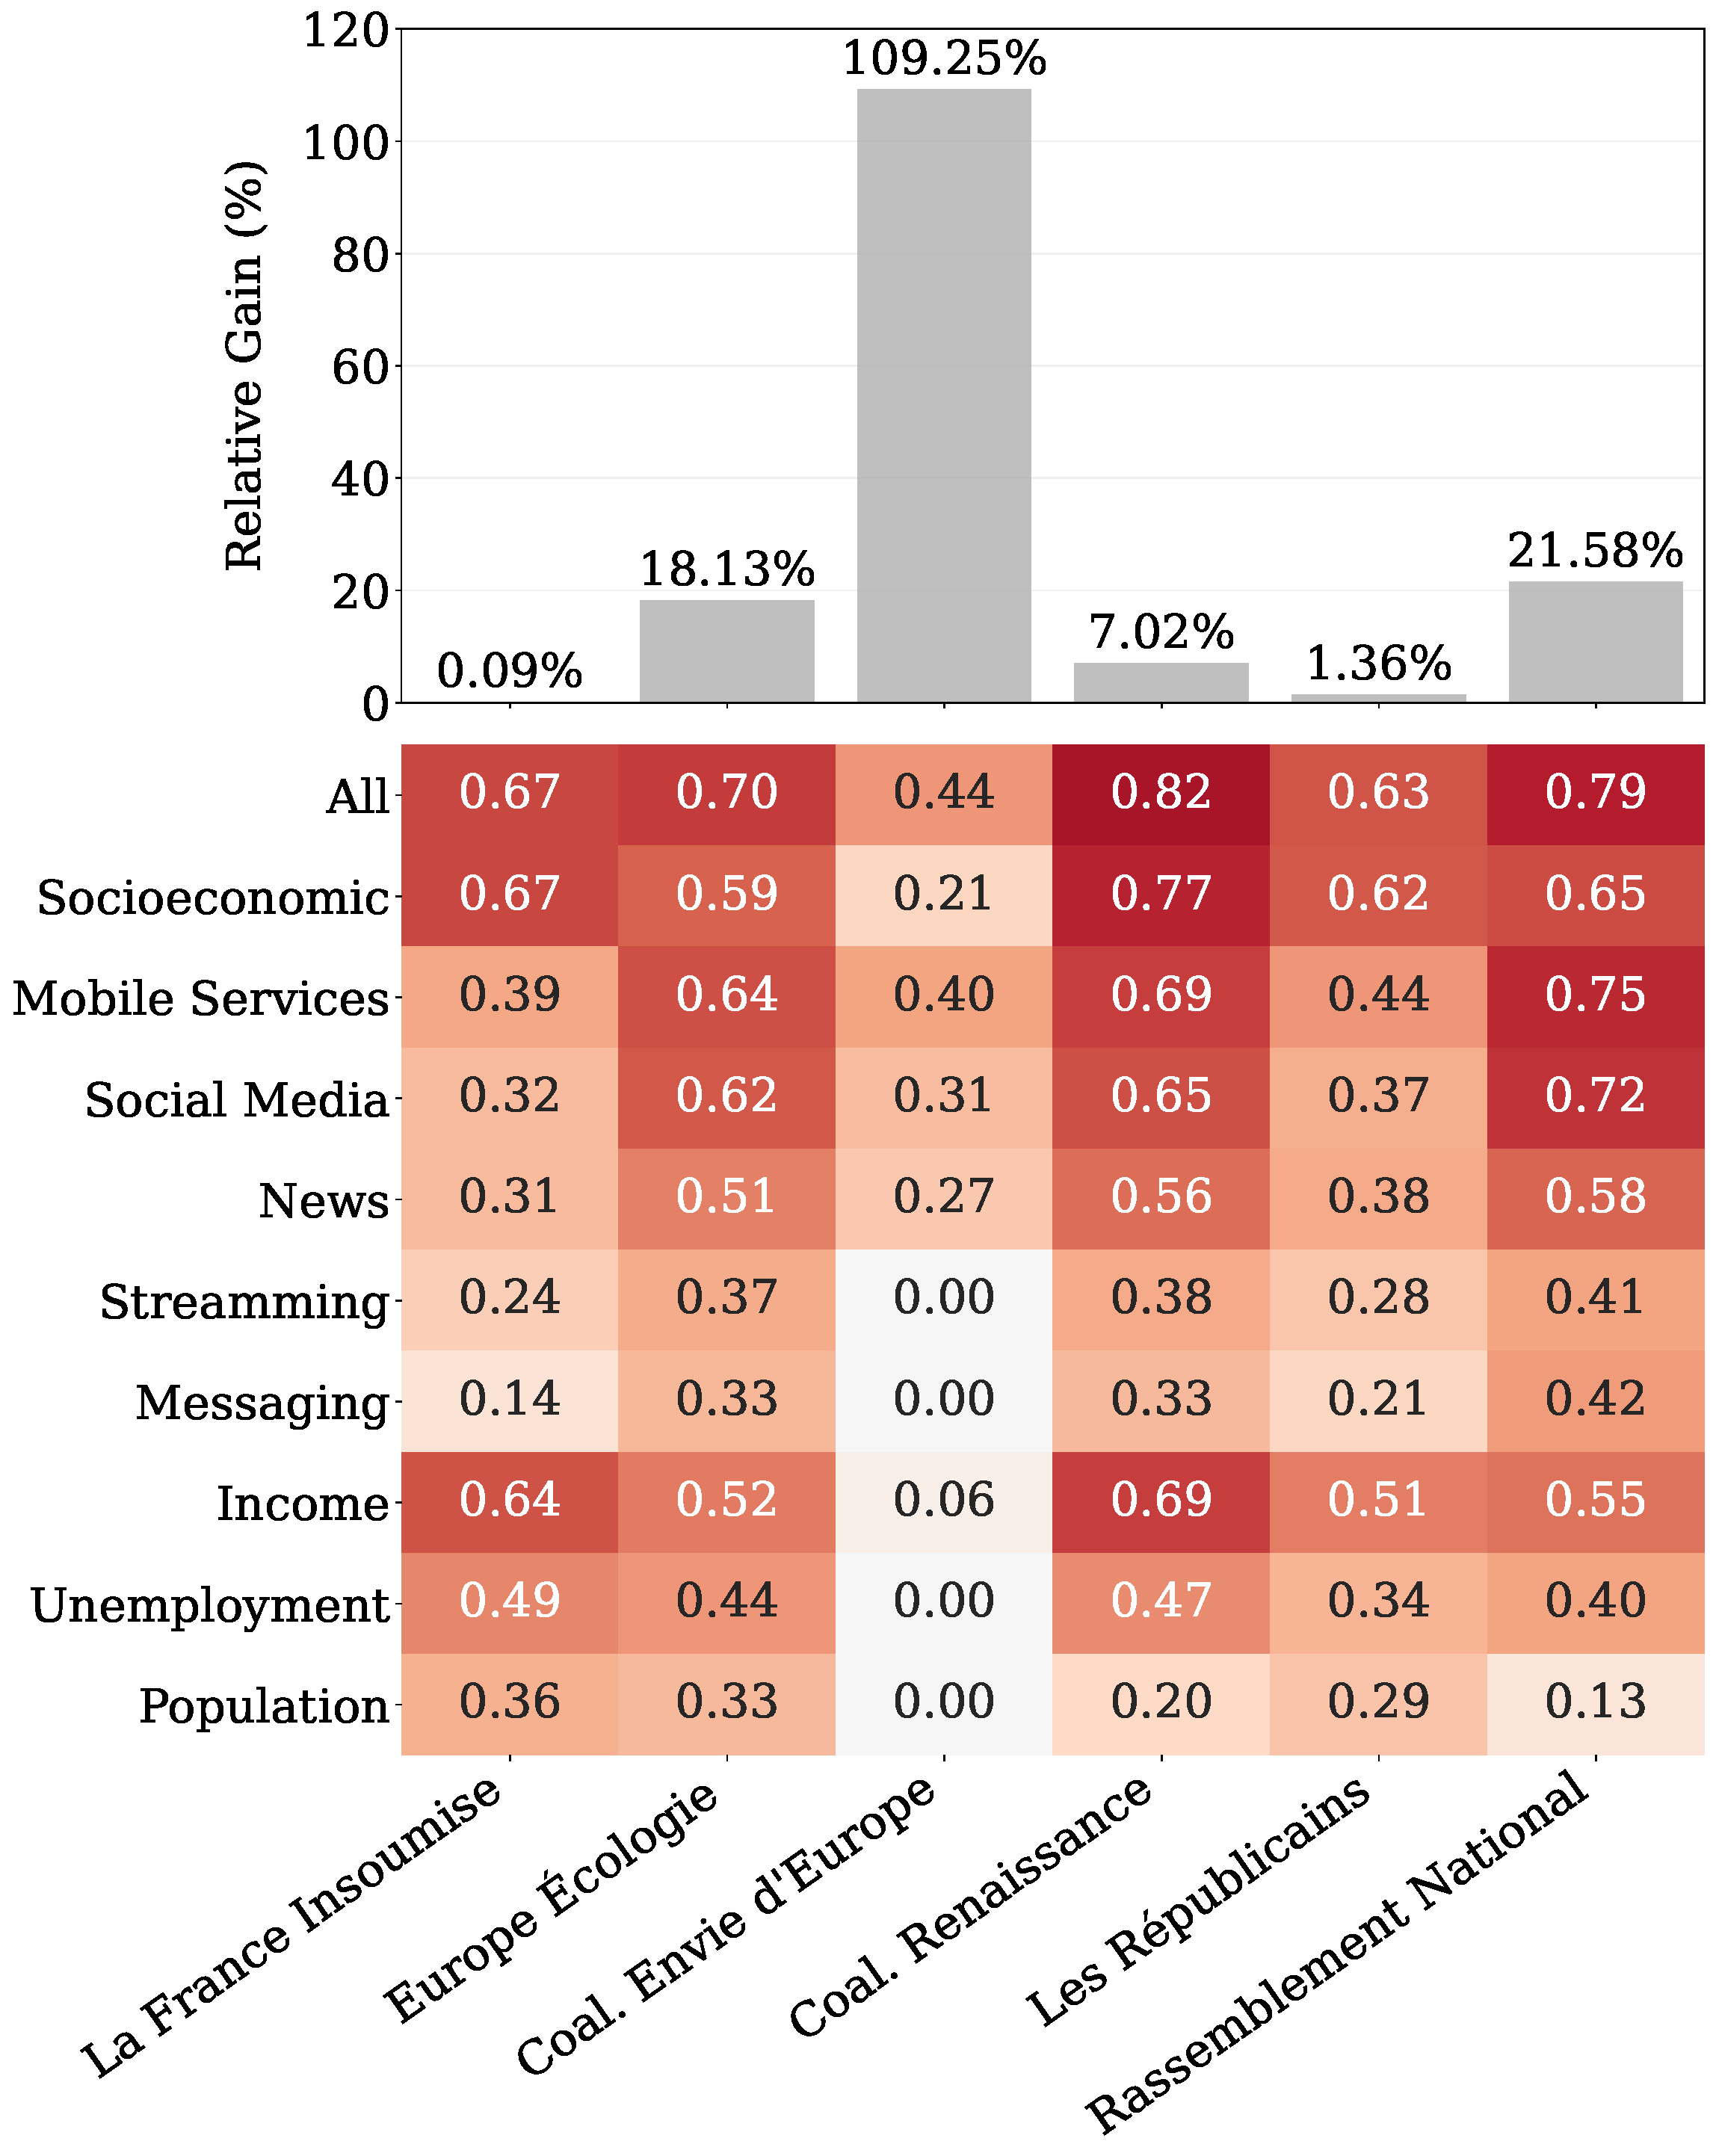
\includegraphics[width=.46\textwidth]{images/dirichlet_regression/rho_relative_gain_europe_2019.pdf}
\label{subfig:election_2019_adj_r2_gain_score}}
\subfloat[2024]{
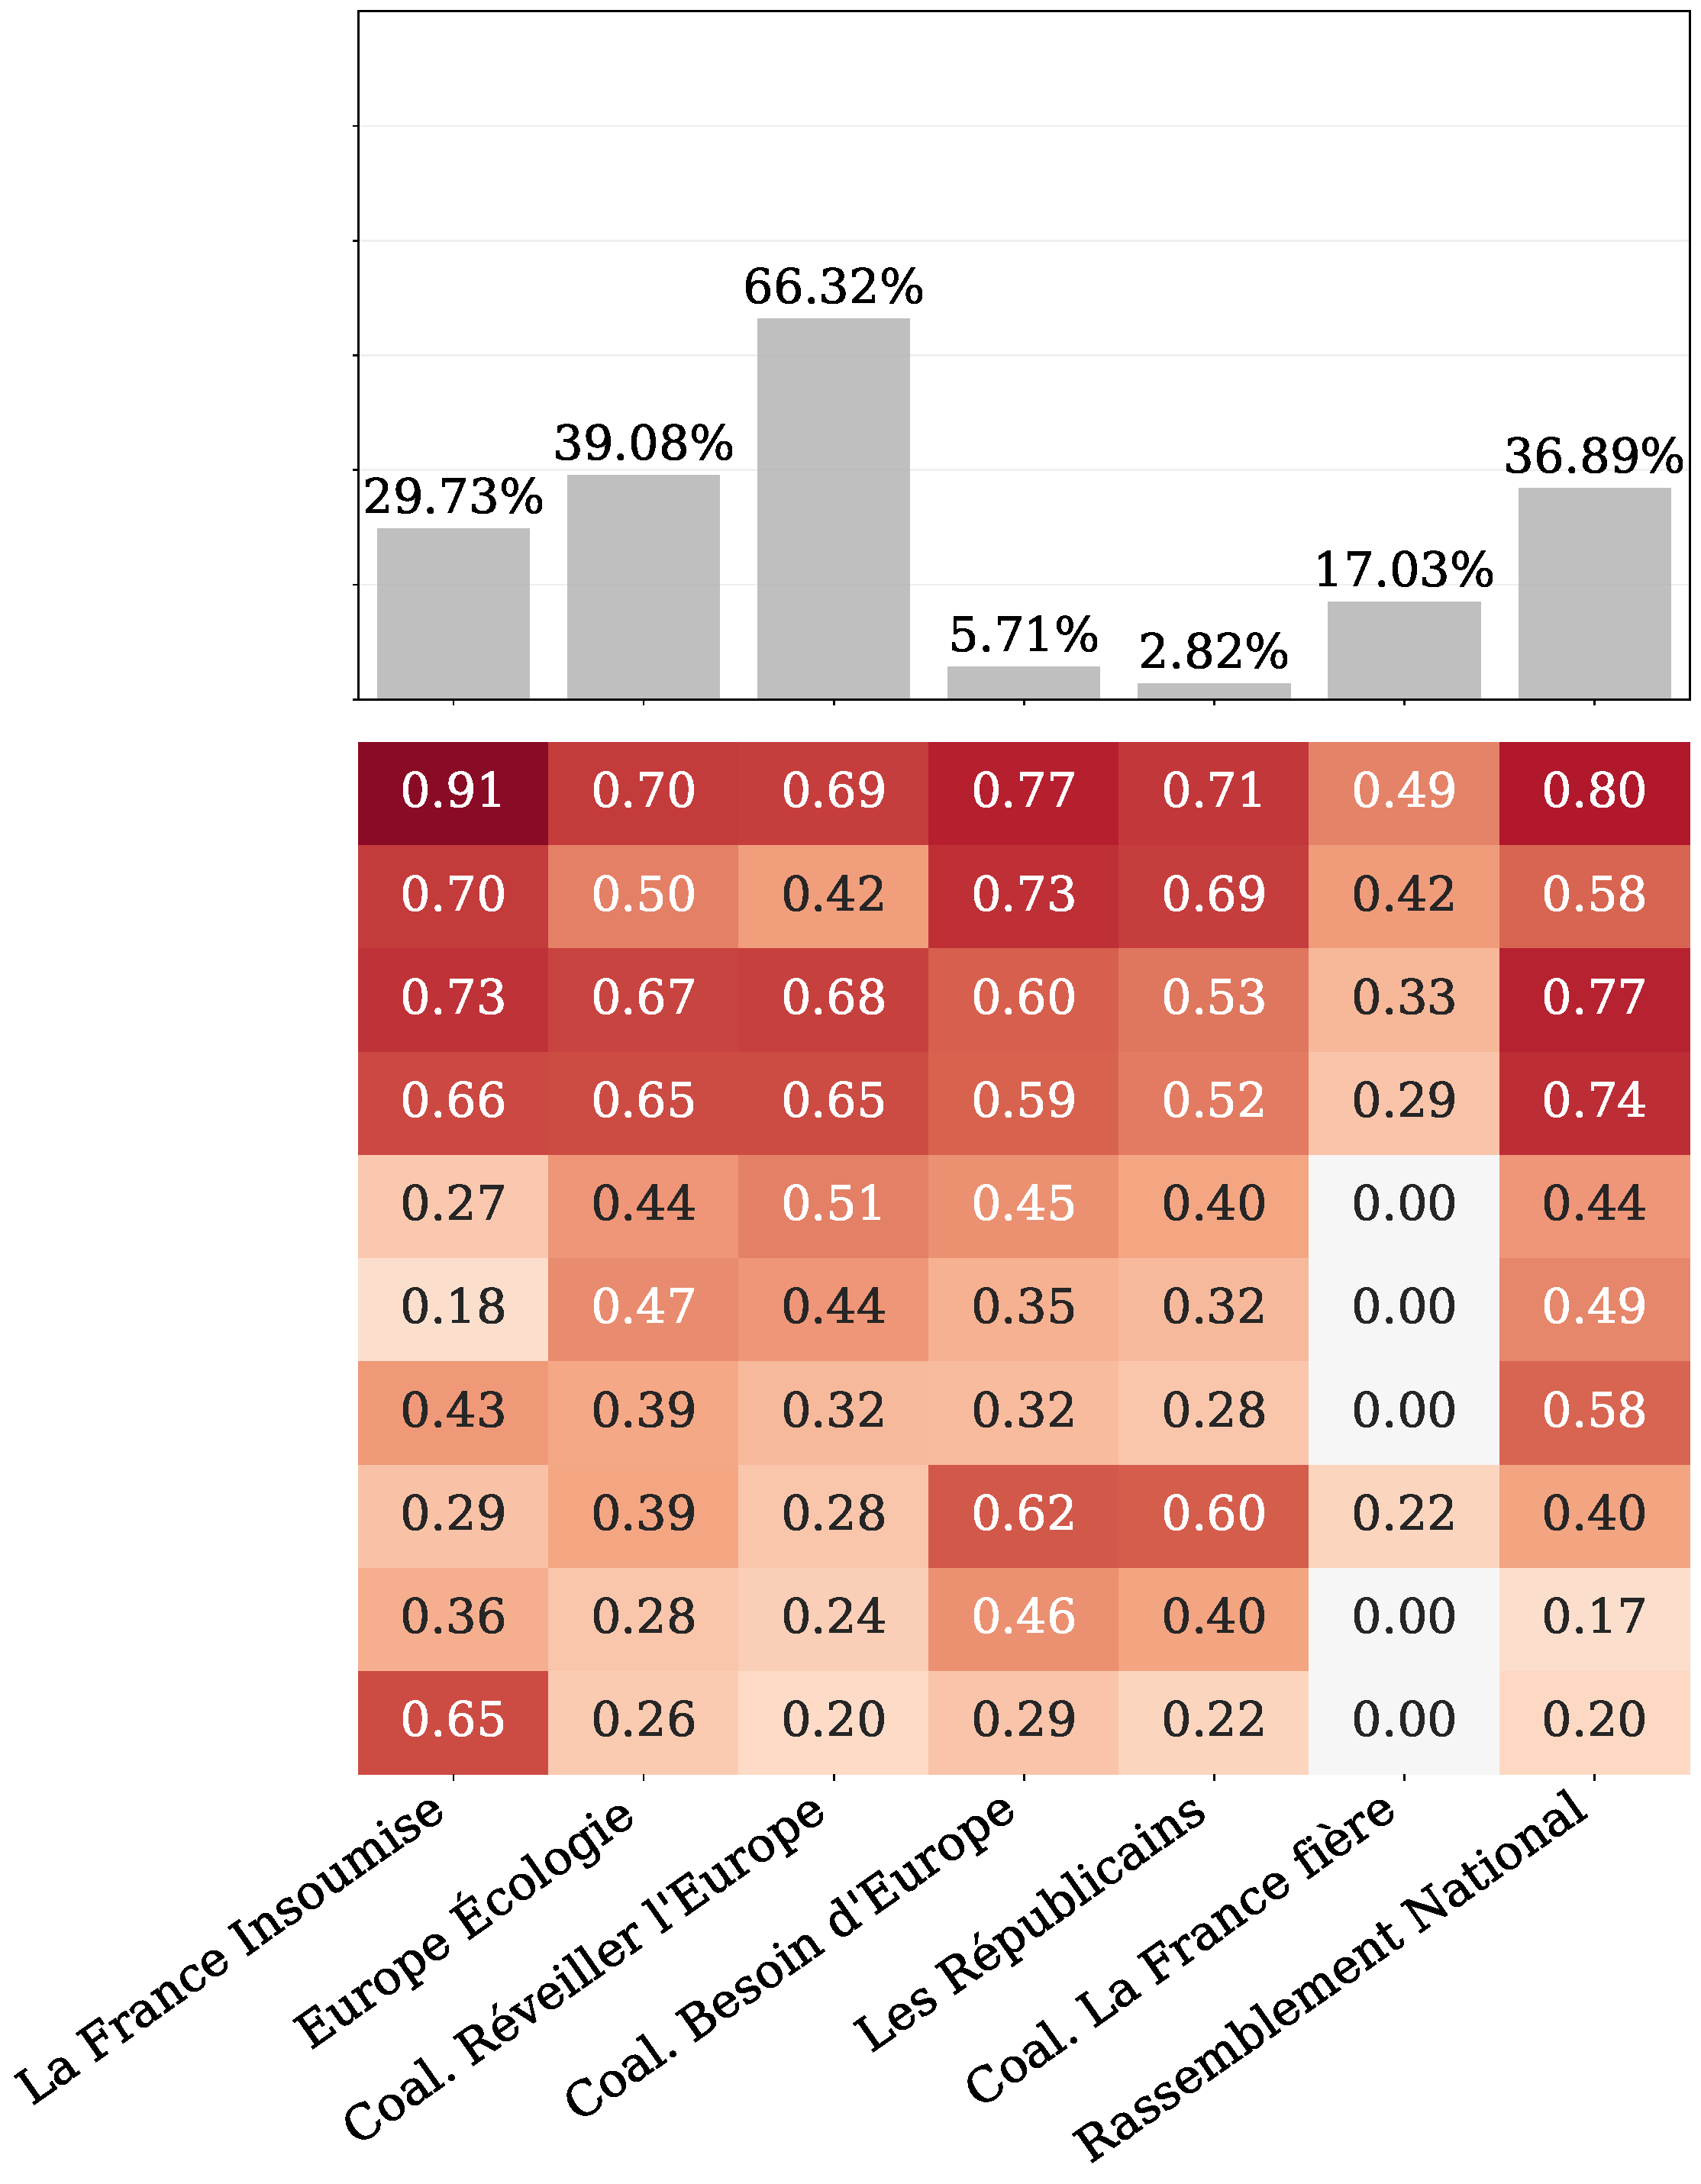
\includegraphics[width=.45\textwidth]{images/dirichlet_regression/rho_relative_gain_europe_2024.pdf}
\label{subfig:election_2024_adj_r2_gain_score}}
% \raggedleft
\hspace{2pt}
\subfloat{
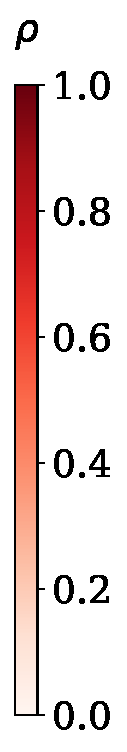
\includegraphics[width=.05\textwidth]{images/dirichlet_regression/colorbar_vertical_rho.pdf}\vspace{50pt}}
\vspace{-8pt}
\caption{Goodness-of-fit across predictor sets and parties.
Bottom:  Correlation ($\bm{\rho}$) values for each model and party. 
Top: Relative gain in $\bm{\rho}$ when adding mobile service variables to the \socioeconomic baseline.
\label{fig:election_adj_r2_gain_score}}
\end{figure*}

Our Dirichlet regressor maximizes likelihood expressed in terms of \adjrsquare so as to abide by best practices in multivariate statistical analysis.
To render the results of the regression more understandable and easily comparable with those attained by the simple pairwise univariate linear models employed in Section~\ref{sec:explain-correlation}, we transform the obtained \adjrsquare values into Pearson's coefficient $\rho$.
Figure~\ref{fig:election_adj_r2_gain_score} reports the 
correlation obtained for each regression model based on the sets of predictor variables summarized in Table~\ref{tab:sets_predictor_variables_election} and political groups across the two elections.

The bottom part of the figure shows the complete matrices of correlation values and lets us observe how the \all model, including the full set of socioeconomic and mobile usage predictors, consistently achieves the highest figures across all parties, attaining $\rho=0.82$ for \RENA in 2019, $\rho=0.91$ for \LFI in 2024, and $\rho=0.80$ for \RN in 2024. Also, the $\rho$ values for the \all model are substantially stronger than those reported for univariate approaches in Figure~\ref{fig:apps_correlation_with_votes}, which highlights the explanatory advantage of the multivariate Dirichlet regression we adopt.
These gains persist after penalizing for additional predictors in~\eqref{eq:political_election_explanation_adj_r2}, and the \ac{AIC}, \ac{BIC}, and log-likelihood in Appendix~\ref{app:aic-bic} corroborate the same ranking.

Indeed, these results allow us to quantify the added value of mobile service demands in capturing multiparty political alignment. To single out that specific contribution, the top panels of Figure~\ref{fig:election_adj_r2_gain_score} show the relative increase in correlation when mobile service variables are added to the \socioeconomic baseline, for all parties and in the two target electoral events.
Essentially, the plots show the percent increment in $\rho$ obtained by the model informed by predictors in the \all set over that achieved by the \socioeconomic indicator set.
In 2019, as shown in Figure~\ref{subfig:election_2019_adj_r2_gain_score}, the gains for \LFI and \LR were marginal; however, the improvements for the rest of the parties were more pronounced with 
increases between $7.02\%$ to $109.13\%$.
Notably, despite the relatively low correlation of \ENVI, the majority of its explained variance came from the \mobile variables, suggesting that digital behavior played a more important role than \socioeconomic variables in explaining its vote distribution.
The 2024 results present an even greater impact of mobile application consumption on the explanatory power of the model: except for the \ENVI 2019 outlier, incorporating digital usages significantly (between $2\%$ and $66\%$) increases the correlation for all parties.
When averaging the gains over all parties, digital usage is associated with a $9.6\%$ and $28.23\%$ increase in mean correlation with vote shares in 2019 and 2024, respectively. For 2019, this figure excludes the \ENVI list, whose very low socioeconomic baseline ($\rho \approx 0.21$) turns a modest absolute improvement into an outlying per-party relative gain; including it raises the 2019 average to $26.24\%$, overstating the result.

\begin{figure}. 
\centering
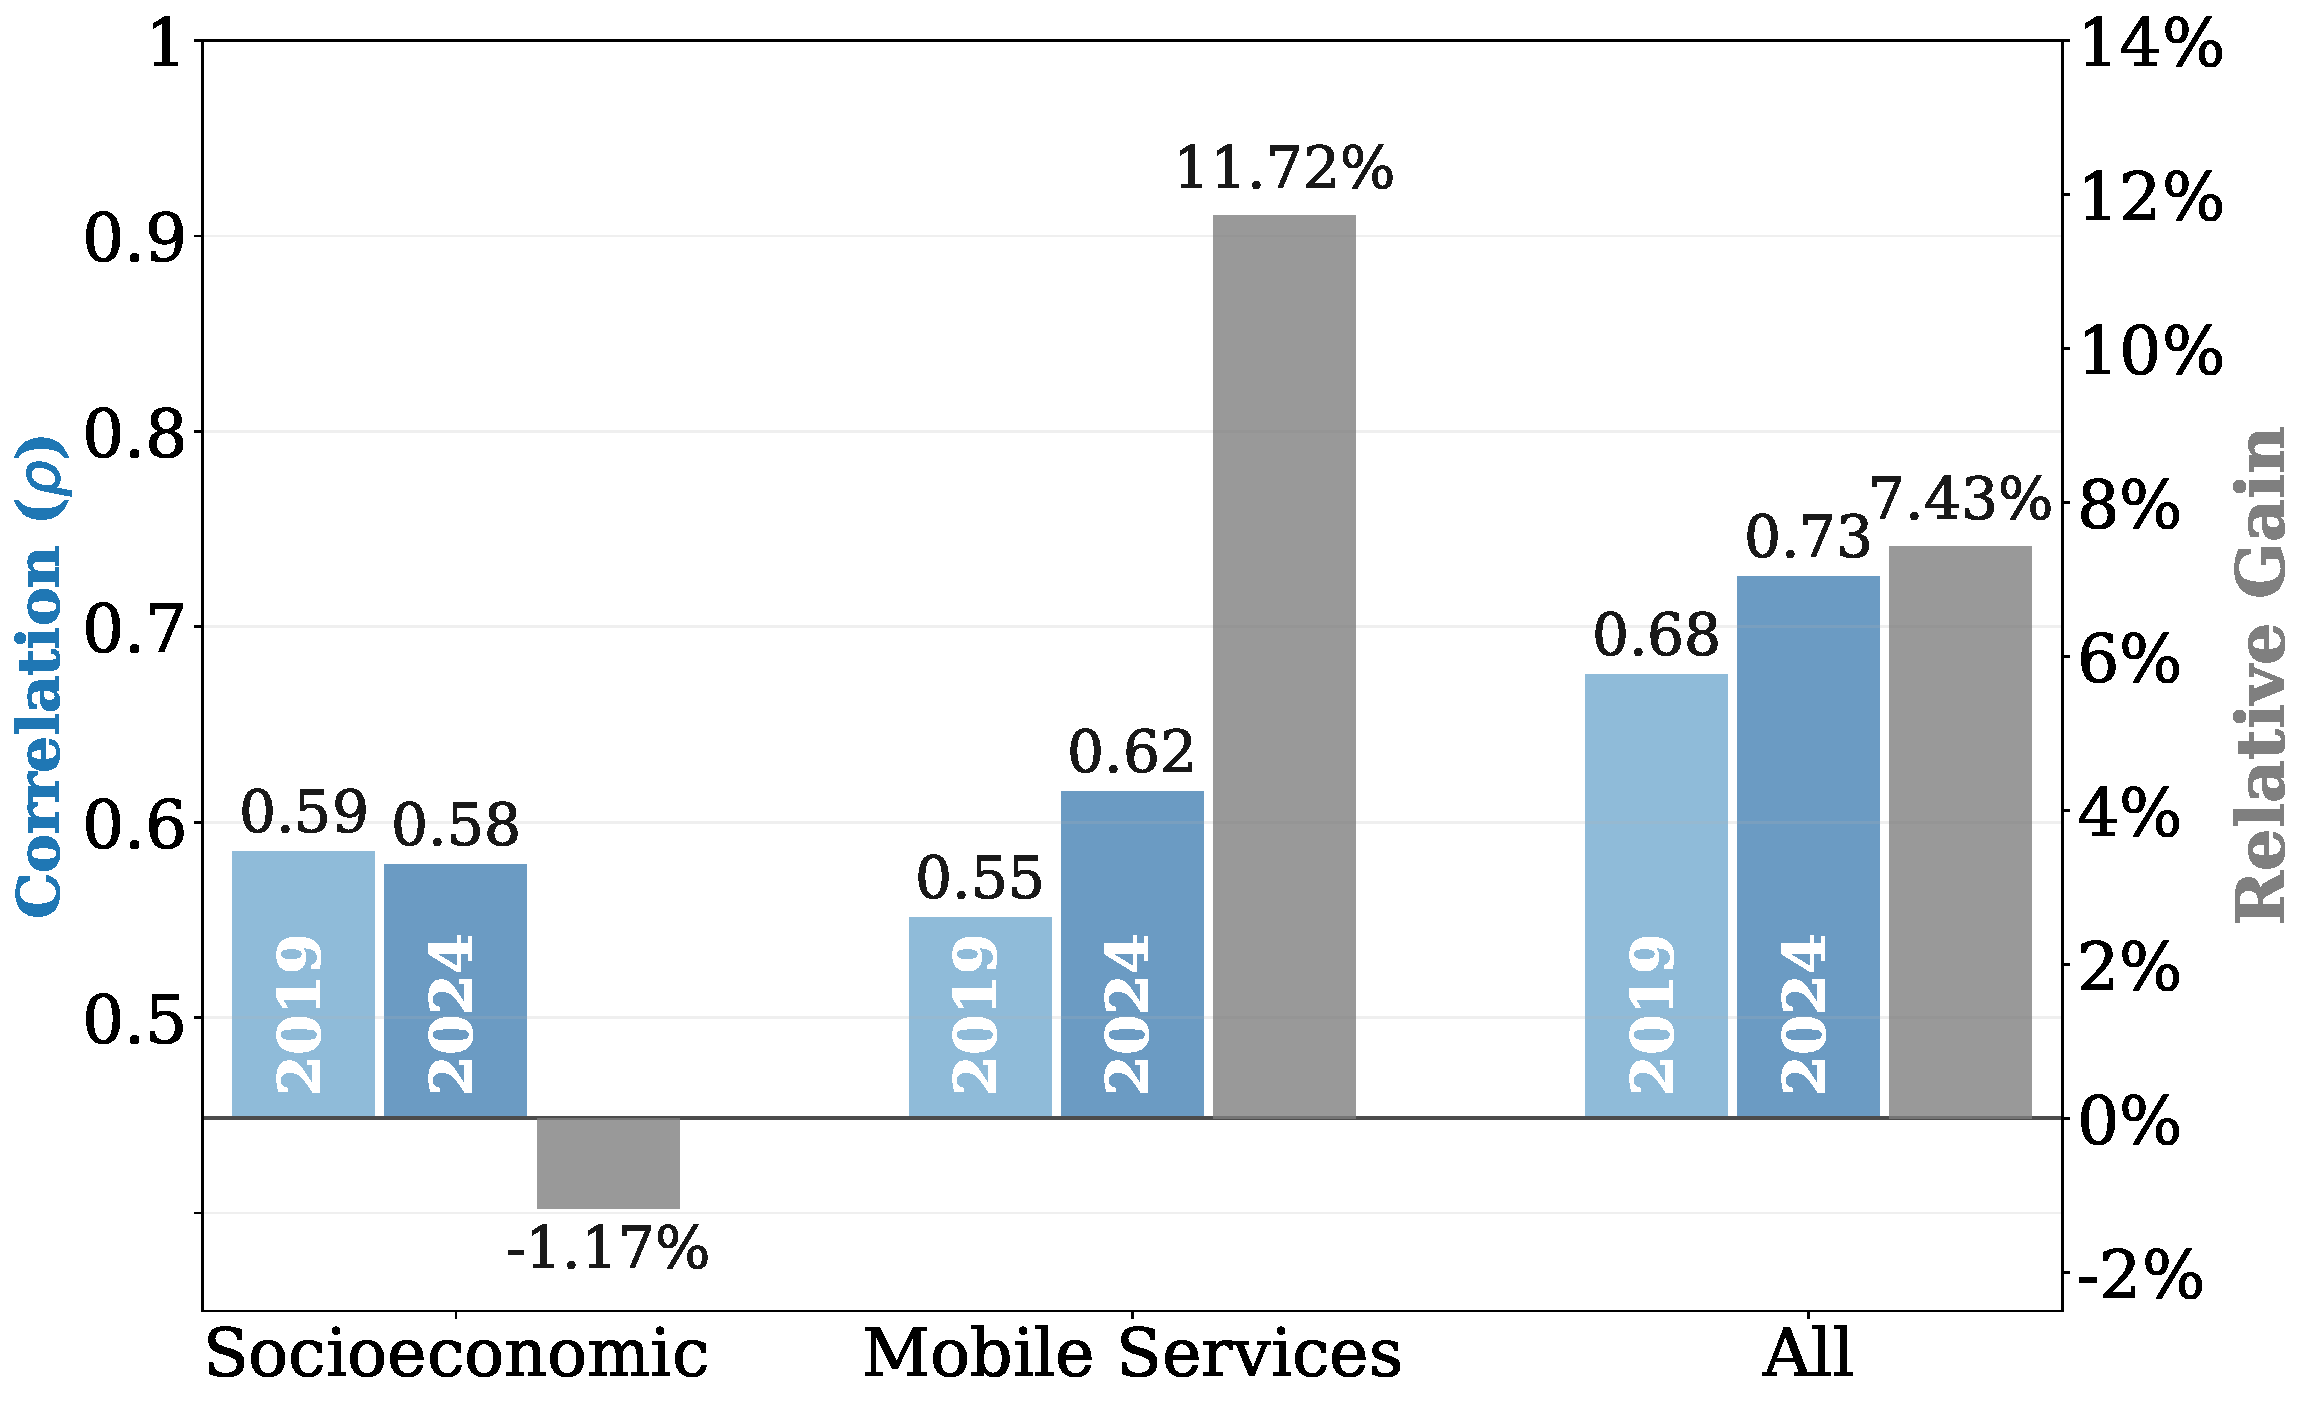
\includegraphics[width=1\linewidth]{images/dirichlet_regression/change_rho_2019_2024.pdf} 
\caption{Change in explainability across elections. Average correlation (right axis) and relative increase in explainability (left axis) from 2019 to 2024.
\label{fig:change_across_year}}
\end{figure}

Our results also enable a longitudinal analysis about how the added explanatory capability of mobile application consumption has evolved in the five years that separate the two target elections.
Figure~\ref{fig:change_across_year} shows the average correlation across all parties for the \socioeconomic, \mobile, and \all models (on the left axis), plus the relative gain in explainability between elections (on the right axis). The striking result is that the \mobile model yields a significant improvement of more than $10\%$ from 2019 to 2024, far outpacing the \socioeconomic indicators, whose explanatory power remains essentially flat; this growth in the digital signal is responsible for the higher \all model accuracy.
Likelihood-based metrics corroborate this trend and reveal an additional qualitative shift: \ac{AIC} and \ac{BIC} results in Appendix~\ref{app:aic-bic} show that \socialmedia alone outperforms the \socioeconomic baseline on all three metrics in 2024, a reversal of the 2019 ranking.

\noindent\textbf{Takeaways.}
\textit{Mobile service usage is associated with facets of political alignment not captured by conventional indicators, improving the accuracy of voting models in multiparty elections. Importantly, this effect seems amplified in recent years, with digital consumption capturing a growing share of voter behavior, while legacy socioeconomic predictors remain essentially stable.}

\subsection{Spatial Analysis}
\label{sec:results-spatial}

\begin{figure*}[t]
\raggedleft

\includegraphics[width=.27\textwidth]{images/dirichlet_regression/maps/colorbar.pdf}
\hspace{0pt}

\centering
%+++++++++Renaissance ++++2019+++++++++++
\subfloat{
\vspace{35pt}
\begin{minipage}{.14\textwidth}
\textsl{Coalition\\Renaissance} (2019)
\end{minipage}}
\subfloat{
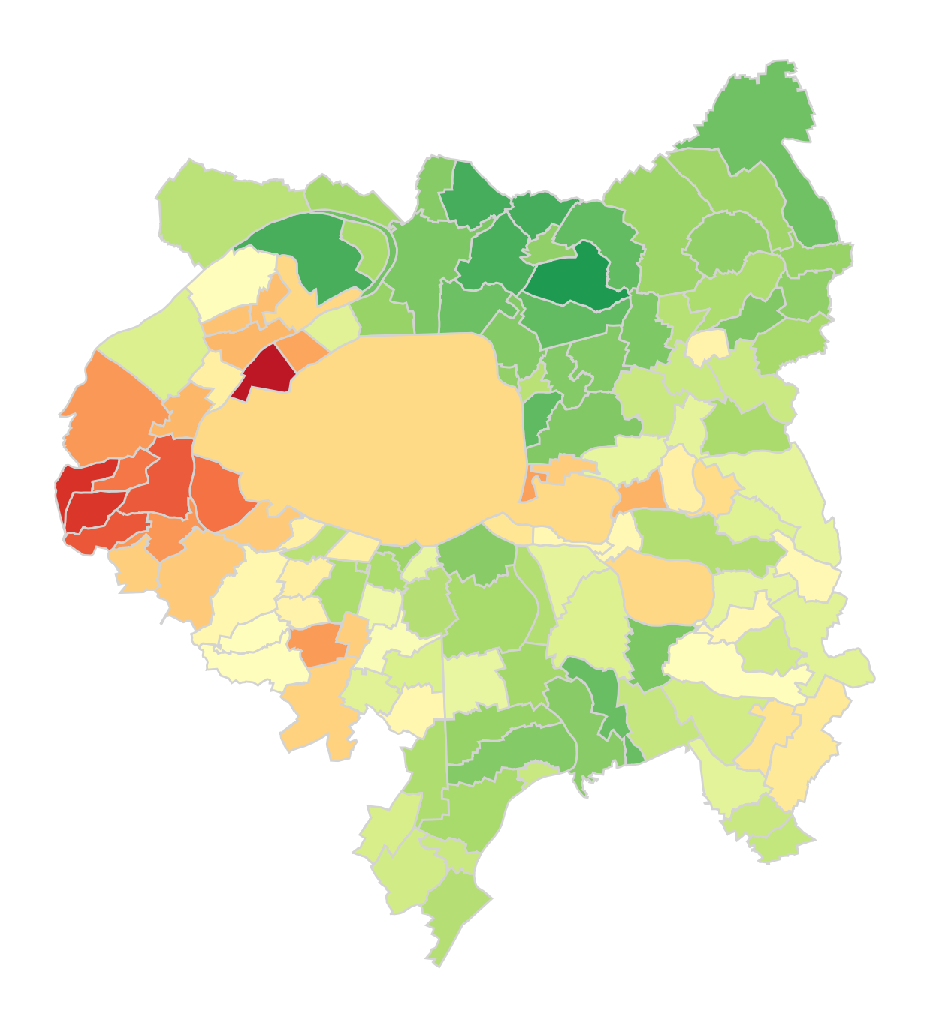
\includegraphics[width=.16\textwidth]{images/dirichlet_regression/maps/ground_truth_Paris_Ren_coal_votes_2019.pdf}}
\hfill
\subfloat{
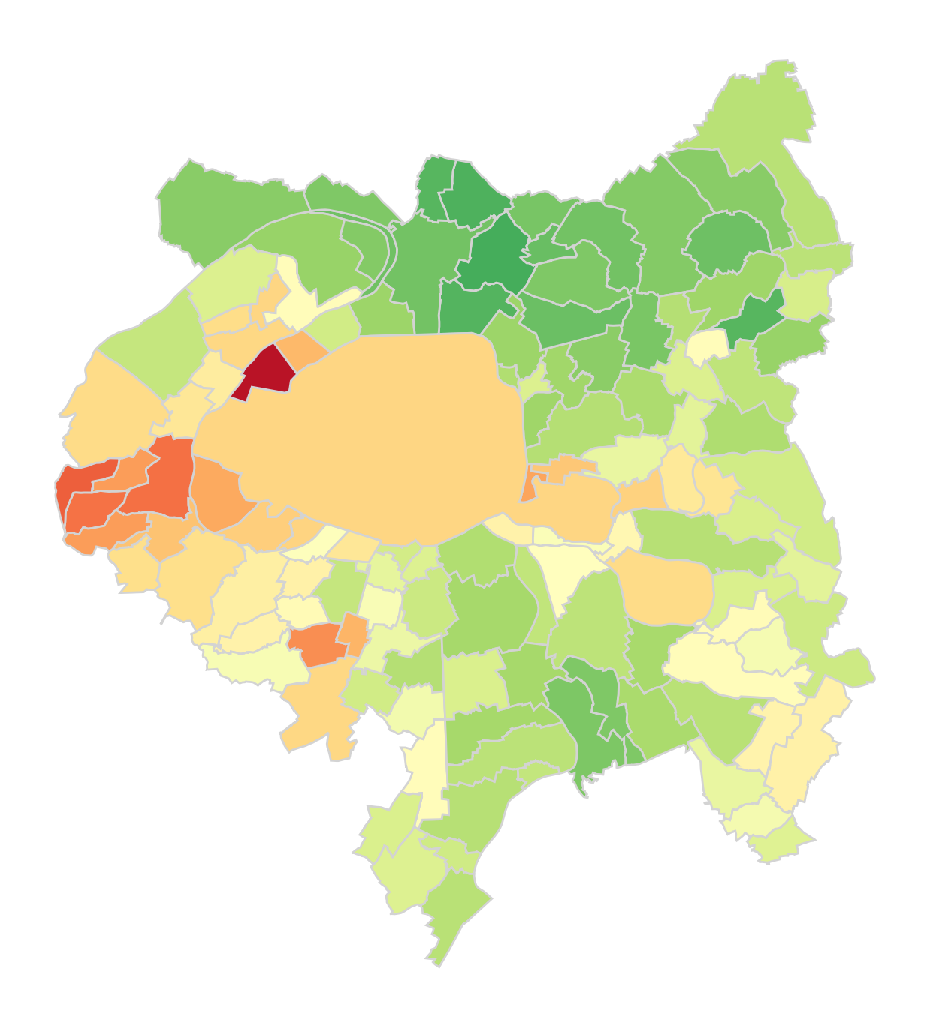
\includegraphics[width=.16\textwidth]{images/dirichlet_regression/maps/prediction_socioeconomic_apps_Paris_Ren_coal_votes_2019.pdf}}
\hfill
\subfloat{
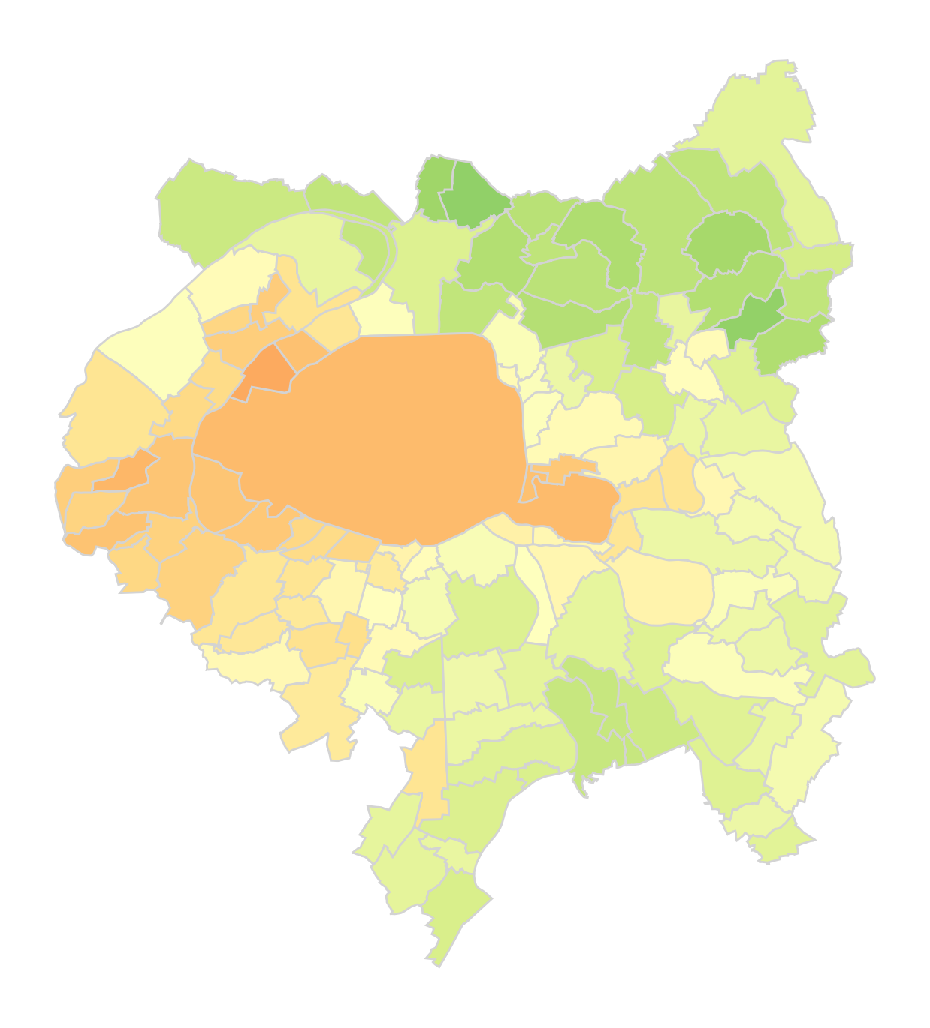
\includegraphics[width=.16\textwidth]{images/dirichlet_regression/maps/prediction_apps_Paris_Ren_coal_votes_2019.pdf}}
\hfill
\subfloat{
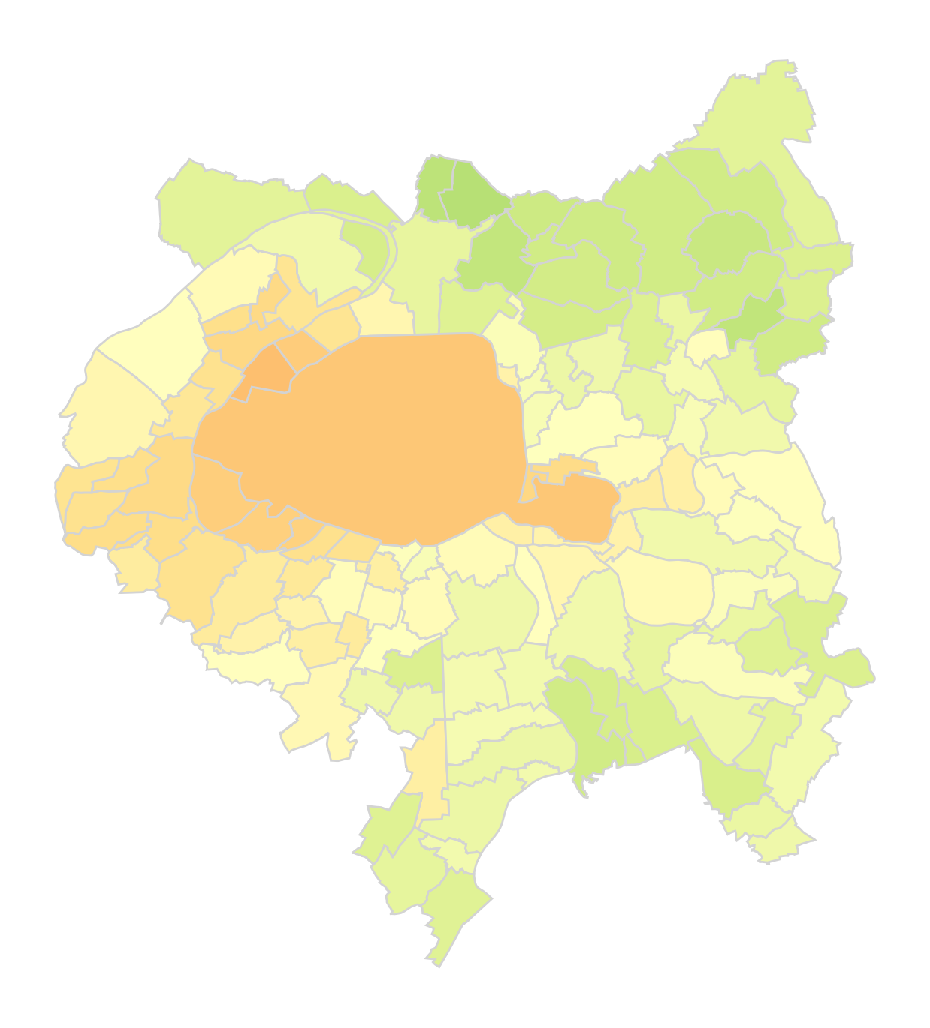
\includegraphics[width=.16\textwidth]{images/dirichlet_regression/maps/prediction_social_media_Paris_Ren_coal_votes_2019.pdf}}
\hfill
\subfloat{
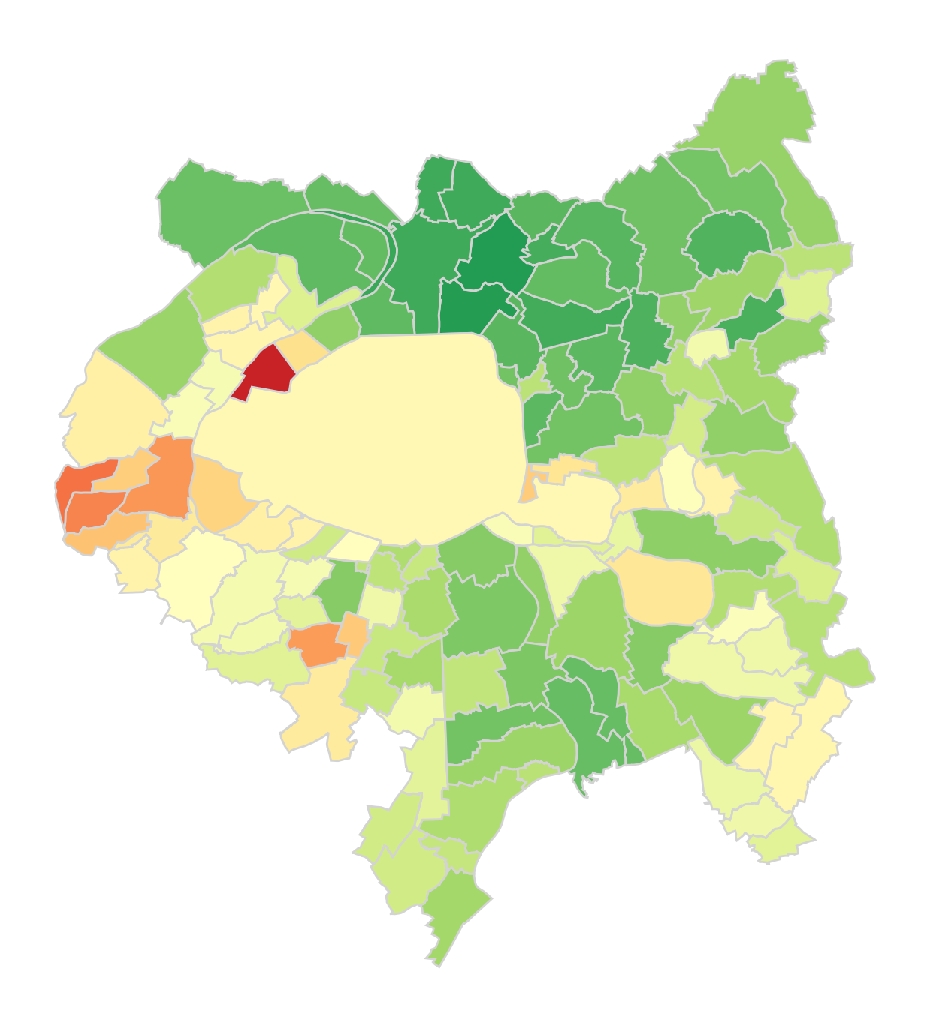
\includegraphics[width=.16\textwidth]{images/dirichlet_regression/maps/prediction_socioeconomic_Paris_Ren_coal_votes_2019.pdf}}


%+++++++++LFI++++2024+++++++++++
\subfloat{
\vspace{35pt}
\begin{minipage}{.14\textwidth}
\textsl{La France\\Insoumise}\\(2024)
\end{minipage}}
\setcounter{subfigure}{0}
\subfloat[Ground truth]{
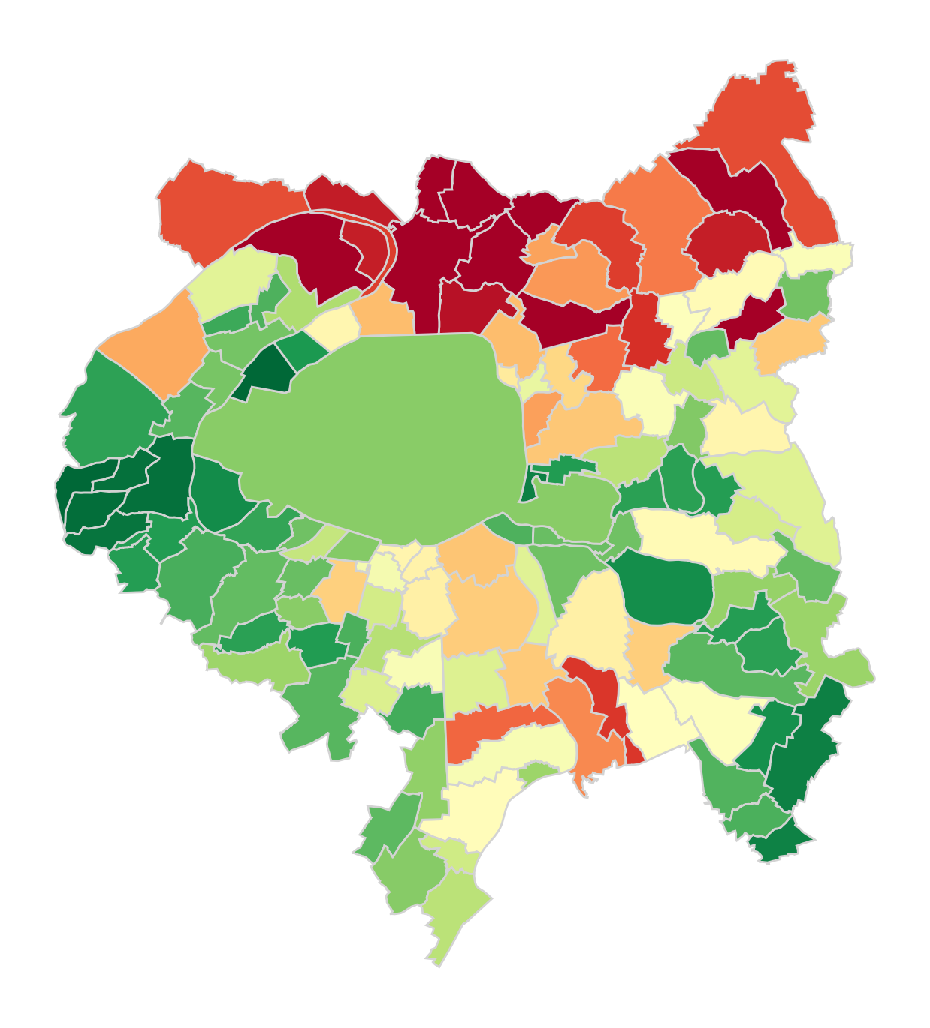
\includegraphics[width=.16\textwidth]{images/dirichlet_regression/maps/ground_truth_Paris_LFI_votes_2024.pdf}}
\hfill
\subfloat[\all]{
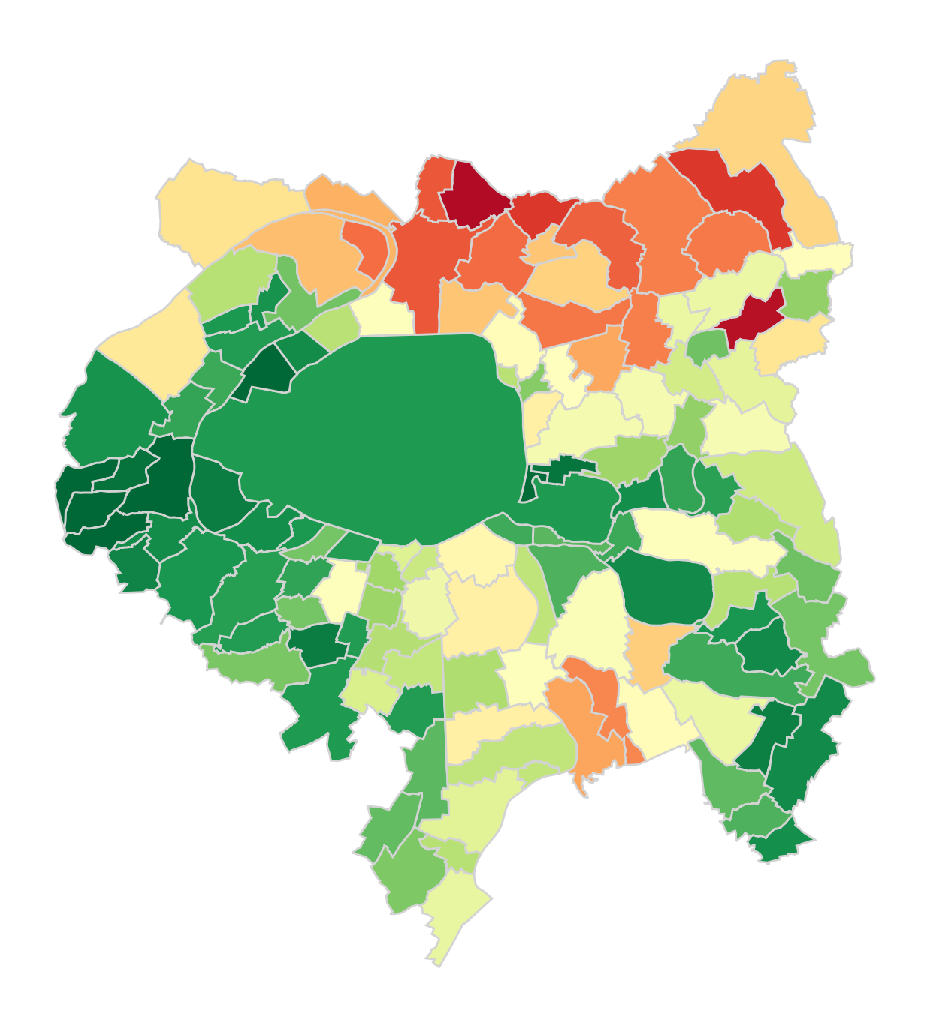
\includegraphics[width=.16\textwidth]{images/dirichlet_regression/maps/prediction_socioeconomic_apps_Paris_LFI_votes_2024.pdf}}
\hfill
\subfloat[\mobile]{
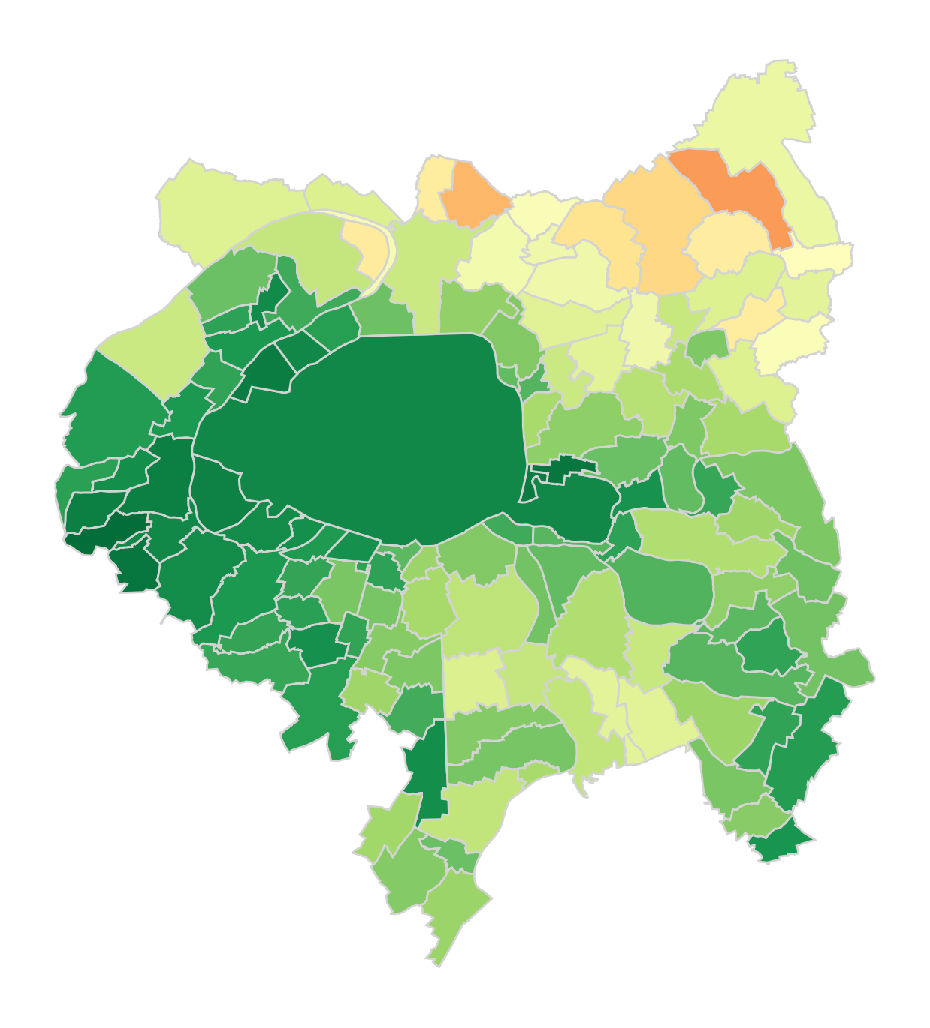
\includegraphics[width=.16\textwidth]{images/dirichlet_regression/maps/prediction_apps_Paris_LFI_votes_2024.pdf}}
\hfill
\subfloat[\socialmedia]{
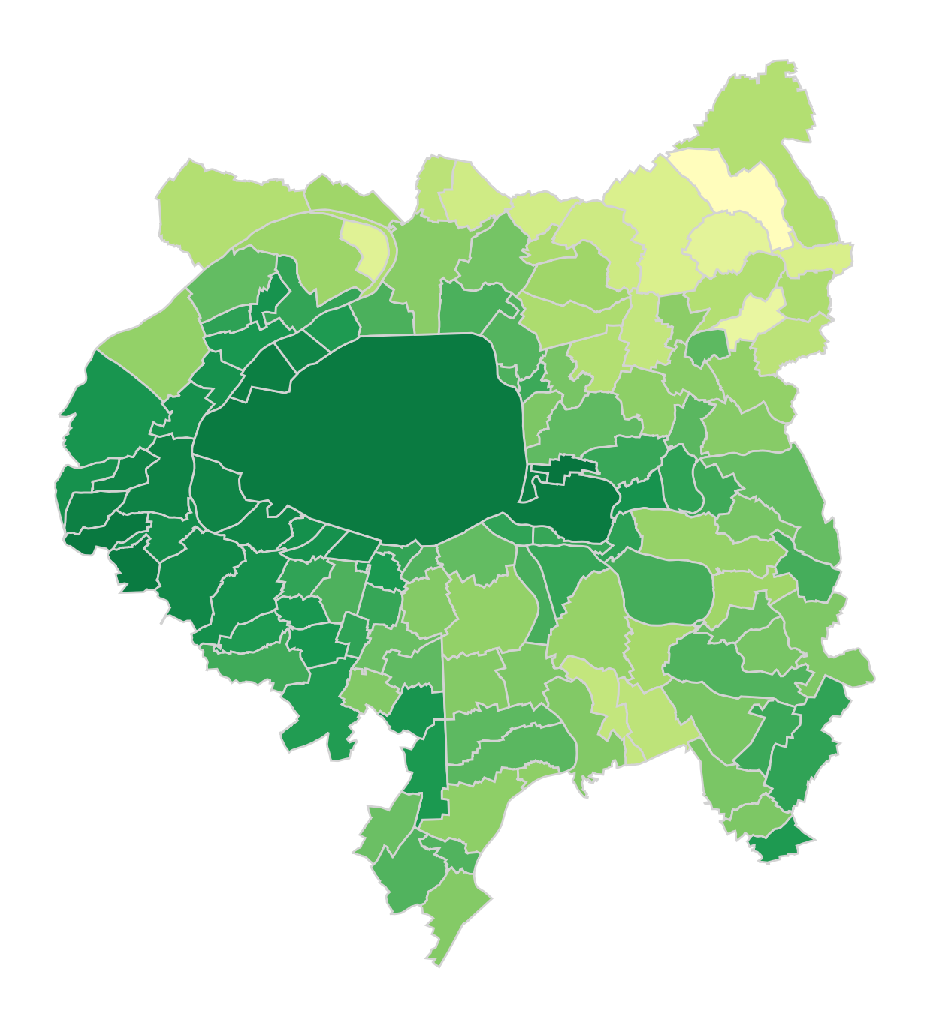
\includegraphics[width=.16\textwidth]{images/dirichlet_regression/maps/prediction_social_media_Paris_LFI_votes_2024.pdf}}
\hfill
\subfloat[\socioeconomic]{
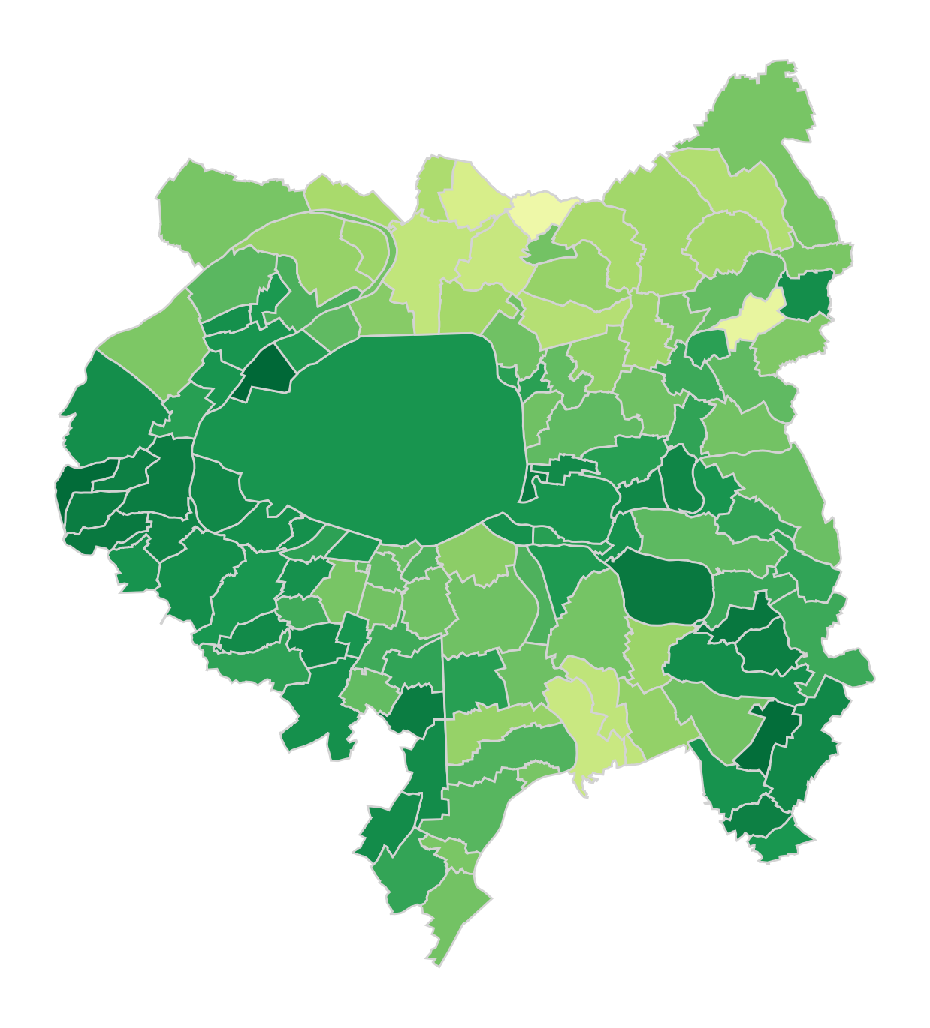
\includegraphics[width=.16\textwidth]{images/dirichlet_regression/maps/prediction_socioeconomic_Paris_LFI_votes_2024.pdf}}
\vspace{-8pt}
\caption{Predicted electoral support in the European Parliamentary elections within the Grand Paris region for two representative parties in 2019 and 2024, respectively.
Panels present (a) the actual vote shares, (b)--(e) predictions from models using four different variable sets from Table~\ref{tab:sets_predictor_variables_election}.
\label{fig:map_predictions}}
\end{figure*}

Beyond the quantitative view provided by the Goodness of fit, Figure~\ref{fig:map_predictions} provides a complementary, qualitative visualization of the capability of the different indicators to capture political alignment.
The top row shows results for \RENA in 2019, while the bottom row shows results for \LFI in 2024 across different models.
While the \all model captures much of the spatial structure in the observed vote shares, the maps also make clear that the contributions of each variable set vary substantially across parties, years, and geographic areas.

The case of \RENA in 2019 illustrates that the \mobile model alone captures part of the spatial pattern of observed votes, mainly driven by \socialmedia variables, yet the \socioeconomic model more accurately identifies specific communes where \RENA received stronger support. The combination of both in the \all model synthesizes these complementary signals.
In contrast, for \LFI in 2024, the \socioeconomic model tends to underestimate vote shares, whereas \mobile appears more informative, successfully capturing communes with high levels of support for \LFI. 

\noindent\textbf{Takeaways.}
\textit{The capability of diverse indicator sets to explain political vote is not homogeneous over space. Instead, specific variables are more or less relevant across geographical areas, paving the way to finer-grained explorations of the added value of mobile application consumption in urban and suburban statistical zones.}

\subsection{Coefficient Analysis}
\label{sec:results-coefficient}

\begin{figure*}
\centering
\subfloat{

\includegraphics[width=.45\textwidth]{images/dirichlet_regression/coefficients_2019_legend.pdf}}
\hfill
\subfloat{
\vspace{2pt}
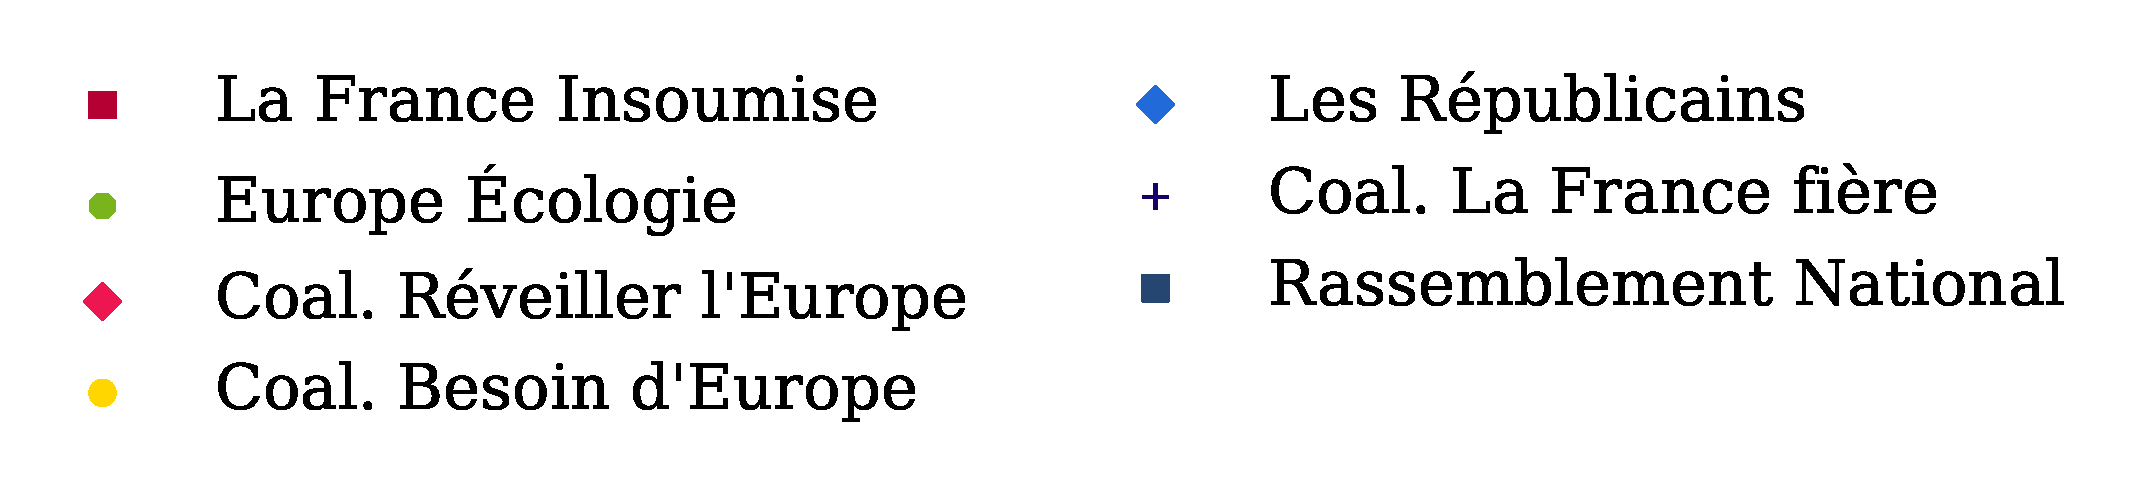
\includegraphics[width=.45\textwidth]{images/dirichlet_regression/coefficients_2024_legend.pdf}}
\vspace{-5pt}

\setcounter{subfigure}{0}
\subfloat[2019]{
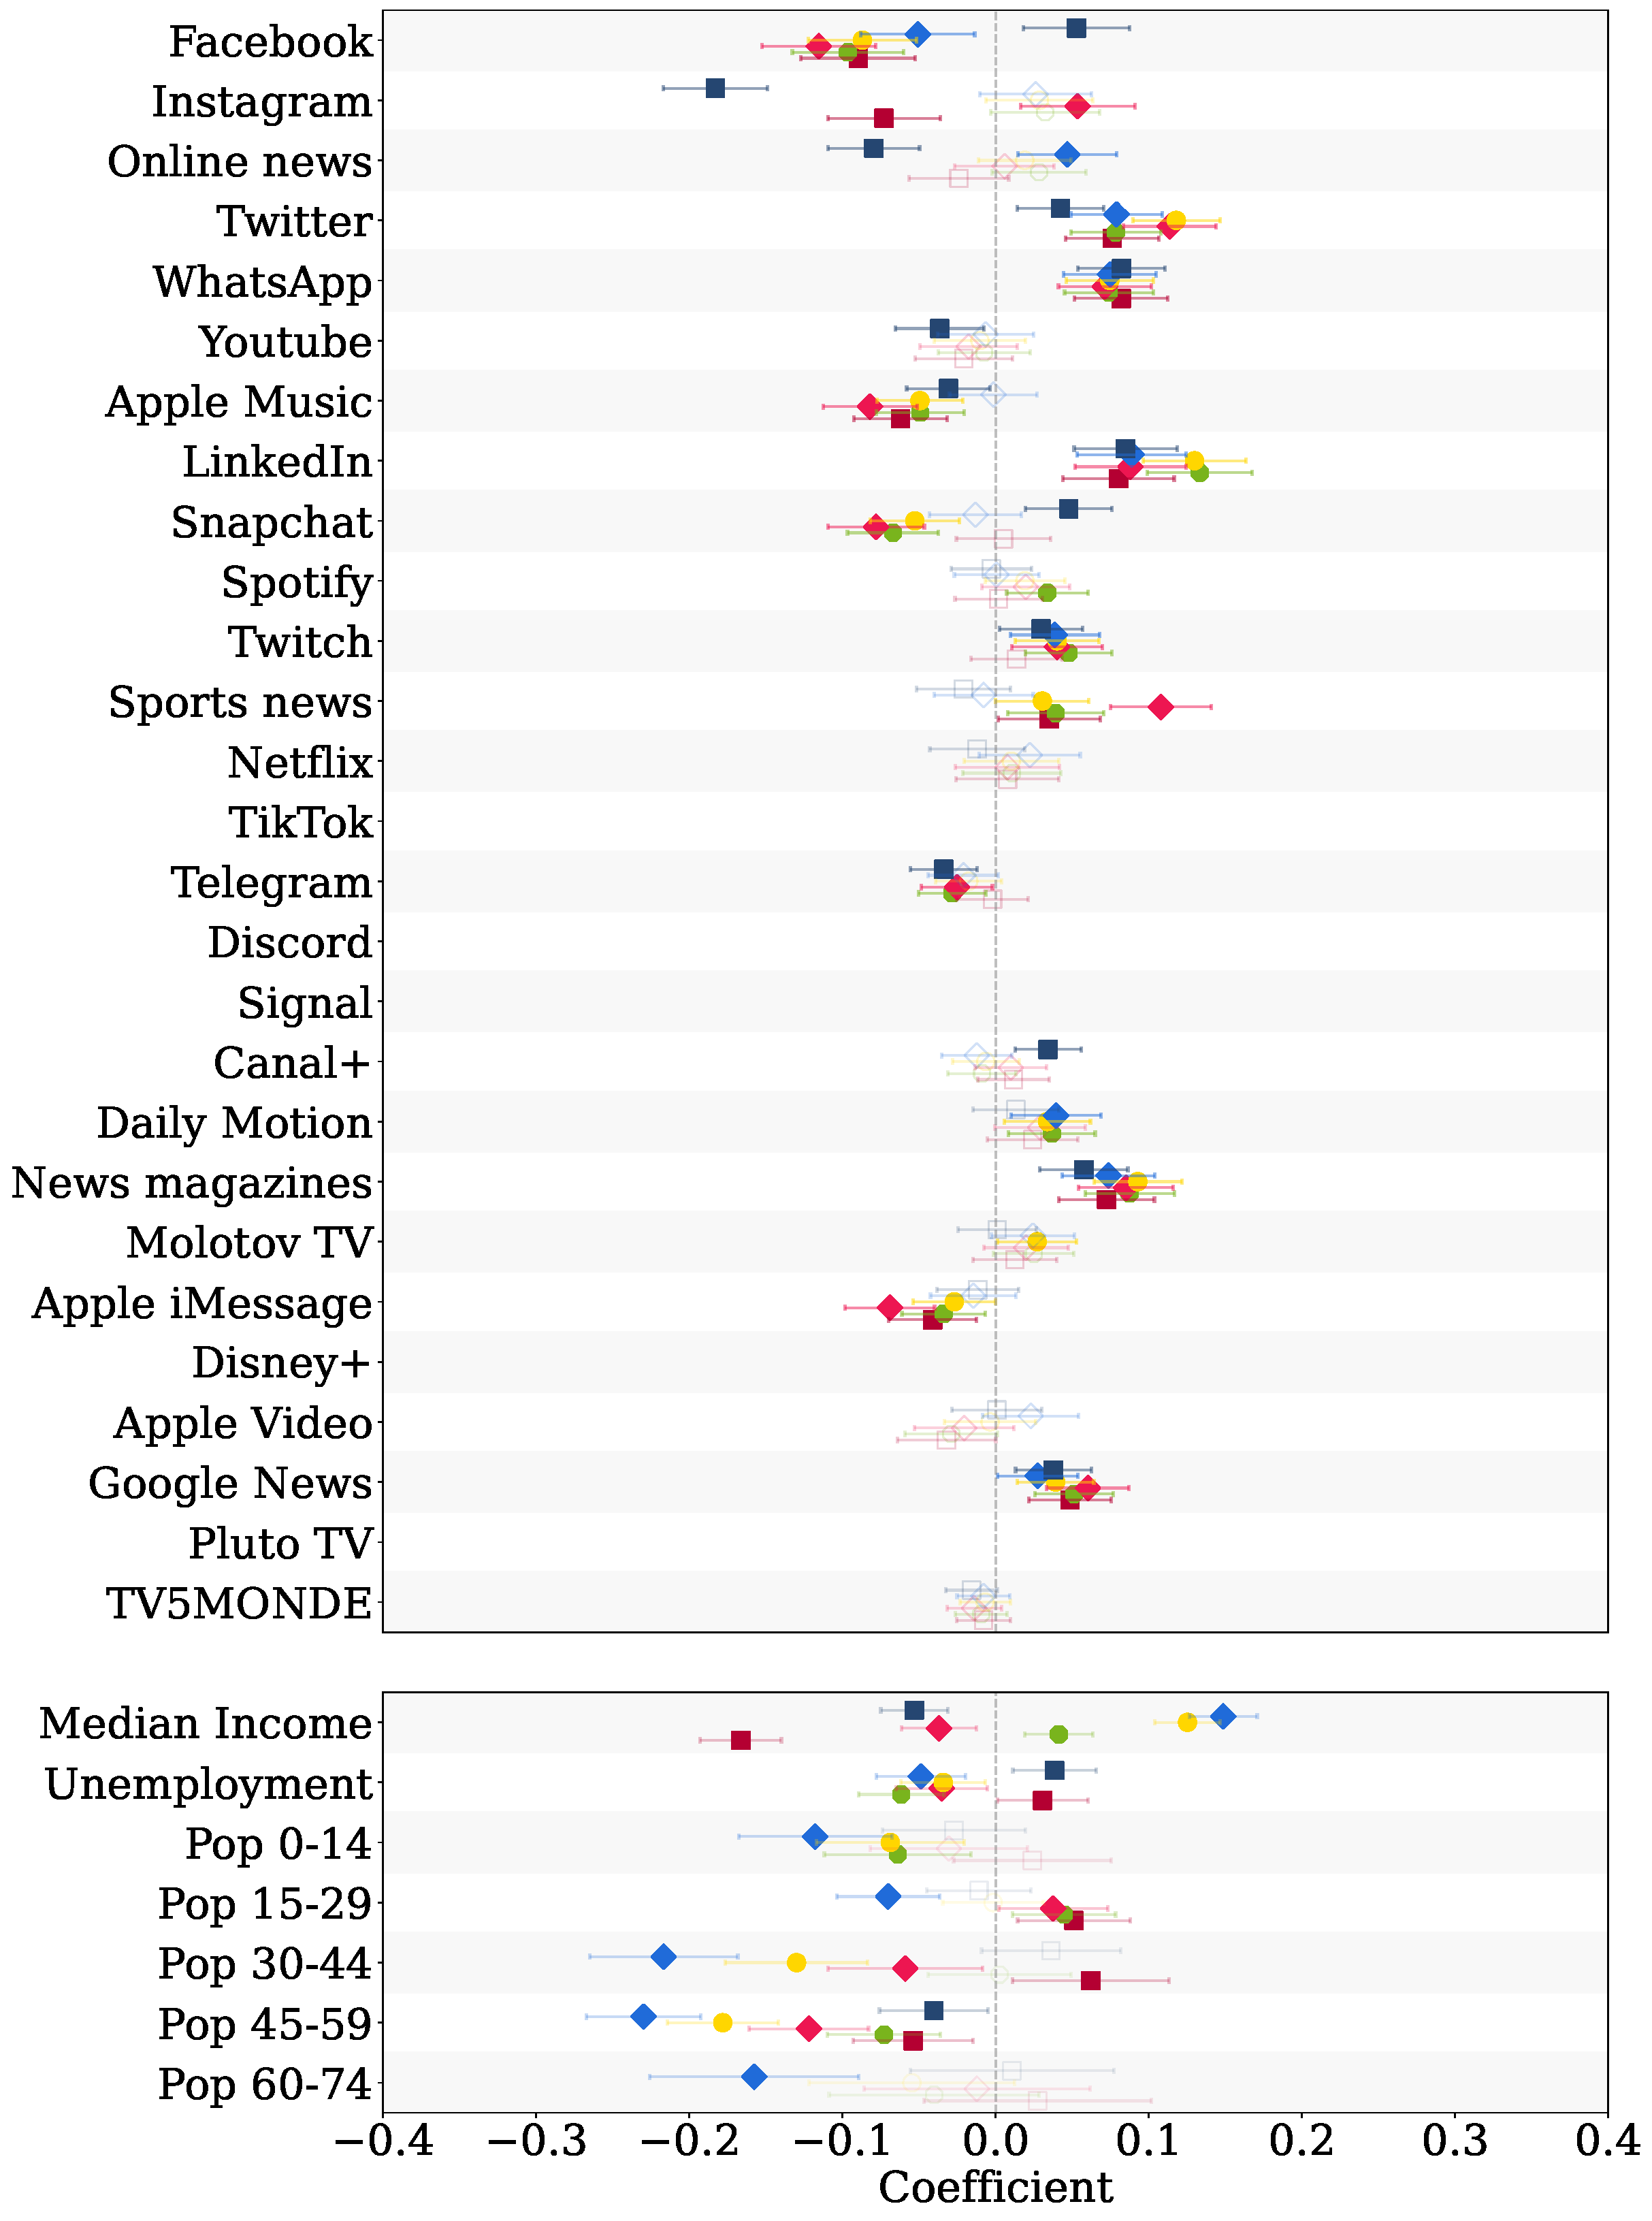
\includegraphics[height=.74\textwidth]{images/dirichlet_regression/coefficients_2019.pdf}}
\hfill
\subfloat[2024]{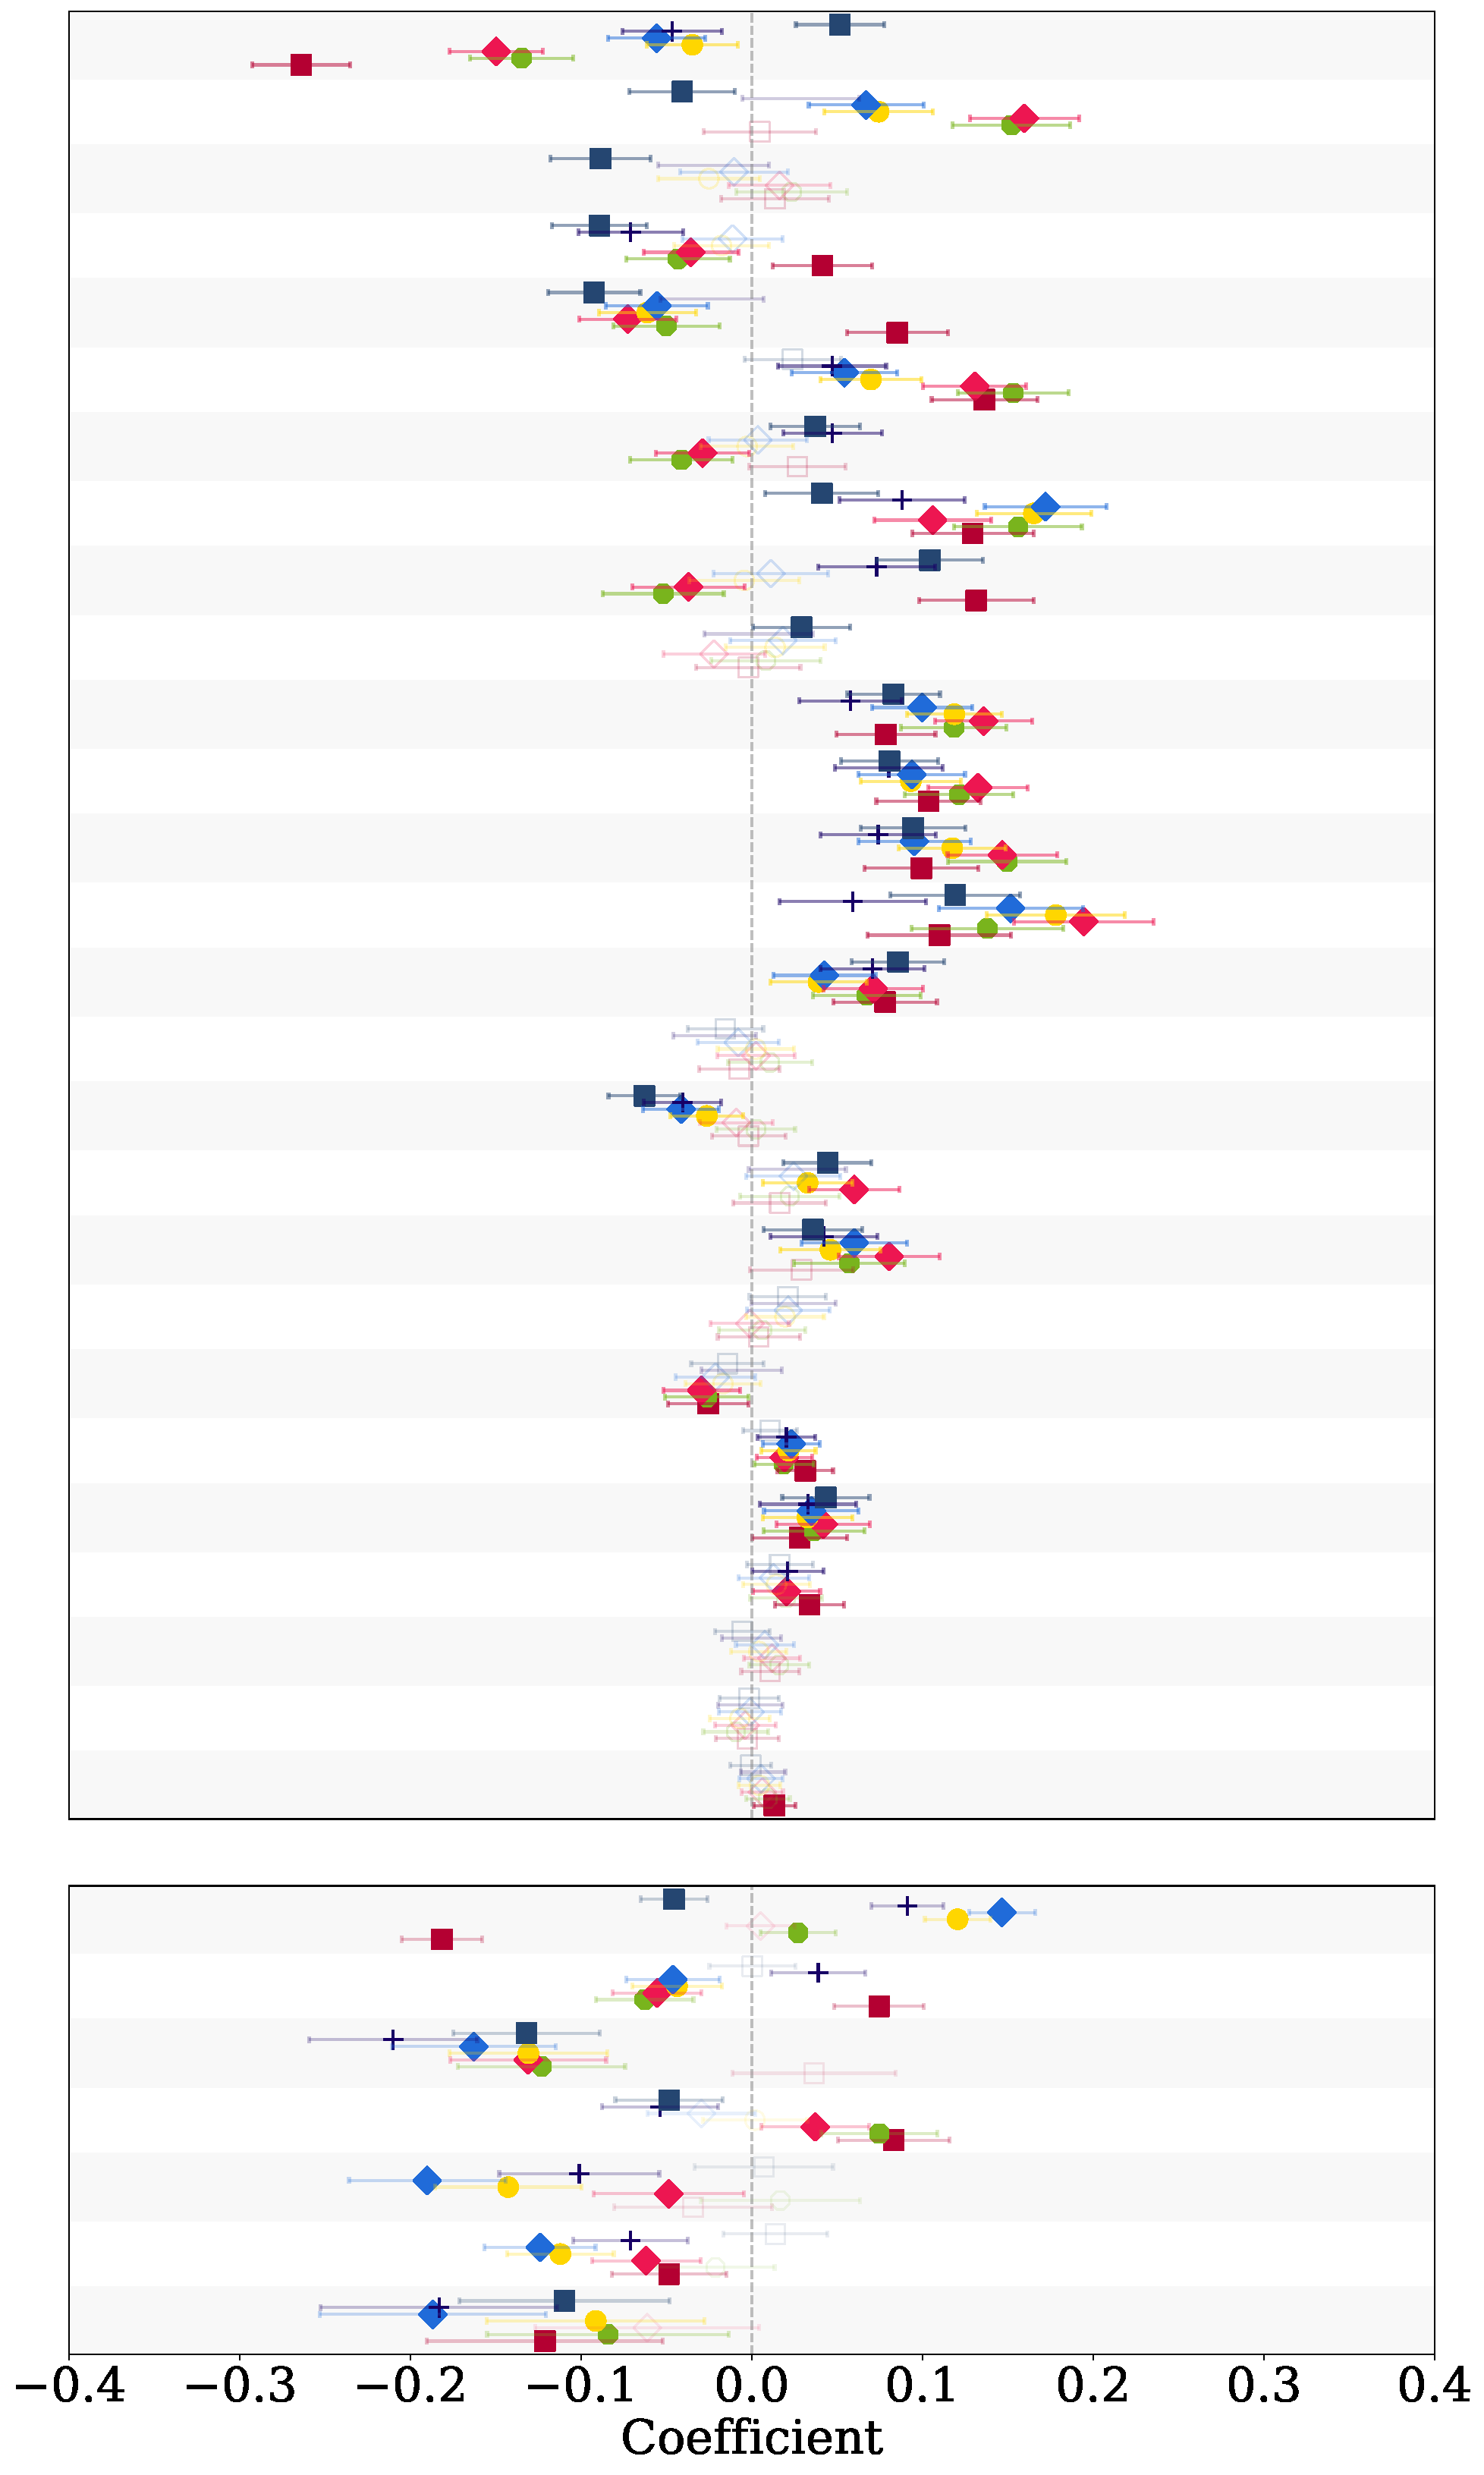
\includegraphics[height=.74\textwidth]{images/dirichlet_regression/coefficients_2024.pdf}}
% \vspace{-8pt}
\caption{Dirichlet regression coefficients for 2019 and 2024. 
Values above (below) zero indicate positive (negative) associations with political alignment. Non-significant coefficients are greyed out.
\label{fig:political_election_explanation_coefficients}}
\end{figure*}


As outlined in Section~\ref{sec:explain-model}, expressing $\alpha$ as a linear combination of predictor variables provides intrinsic interpretability, similar to standard linear regression.
This design choice lets us derive Figure~\ref{fig:political_election_explanation_coefficients}, which presents the regression coefficients $\beta_q$ of the \all model that integrates both socioeconomic indicators and mobile service consumption.
By examining these coefficients, we can assess how each variable relates to party vote shares and identify which services are associated with higher or lower electoral support.

Since the Dirichlet regression maximizes the log-likelihood, the resulting formulation can be interpreted analogously to a linear model in log-space, where the vertical line at $x=0$ marks the threshold for coefficient significance.
Positive coefficients indicate a direct relationship with vote share (higher consumption, more votes), while negative ones indicate the opposite.

To account for statistical uncertainty, we report $95\%$ confidence intervals (horizontal error bars) and exclude variables whose intervals overlap zero, as they do not significantly impact any party’s vote share.
Because socioeconomic variables are explicitly included, the coefficients associated with mobile service demand reflect the unique contribution of each application, disentangled from its potential effects as proxies to the underlying socioeconomic conditions.
From the results in Figure~\ref{fig:political_election_explanation_coefficients}, we draw the following points.

\noindent\textbf{Median Income.} 
Household median income plays a significant role in explaining political alignment and is a key variable for all parties except \REVE in 2024.
While relatively consistent across both elections, it relates strongly to \LFI and \LR, as well as \RENA in 2019 and \BESO in 2024.

\noindent\textbf{Facebook and Instagram.} 
The social media platforms that play a major role in political alignment are Facebook and Instagram, with relatively positive behavior.
On one hand, higher Facebook usage consistently correlates with more votes for \RN across both elections, while it is negatively associated with the vote shares of all other parties. 
On the other hand, areas with higher Instagram usage tend to favor moderate and centrist parties, such as \ENVI in 2019 and \REVE, \EEC, \BESO, and \LR in 2024.
In a complementary manner, lower Instagram demand is associated to higher political alignment for extremist Left and Right parties like \RN and \LFI.

Several of these temporal shifts admit plausible interpretations; we offer them as hypotheses for future empirical validation rather than established findings.

\noindent\textbf{Twitter.}
Twitter exhibits a notable shift across elections. In 2019, it is a significant predictor for all parties, being particularly popular among centrist parties like \RENA and \EEC. 
However, in 2024, Twitter loses its alignment with centrist parties and instead shows a clear polarized pattern: higher use of the application becomes associated with \LFI, while areas with lower Twitter consumption match those where \LFF and \RN received more votes. 
Previous work~\cite{haapala2023disrupting} has reported on the successful Twitter campaign launched by Manon Aubry after the 2019 elections, based on the concept of \textit{raising awareness} and promoting among users of the platform her image as a disruptive outsider in the French political scenario, which may explain the observed shift.

\noindent\textbf{TikTok.} 
While we lack a 2019 reference point for TikTok, the 2024 results show it is most strongly associated with \RN, followed by \LFI (both extreme parties) and \REVE (moderate-left). These results suggest the application, widespread among younger voters, may have a role in polarizing political alignment~\cite{cartes2025attracting, algan2025fievre}.

\noindent\textbf{Netflix and Spotify.} 
Some apps are not significant predictors in 2019 but become relevant for certain parties in 2024. 
Notably, both Netflix and Spotify are insignificant to all parties in 2019 but became relevant in 2024; in particular, Spotify becomes a significant predictor for almost all parties. 
One possible explanation is the growing emphasis on podcasts in both platforms, supported by major deals with popular political commentators~\cite{spotify_joe_rogan} and a collaboration agreement with Radio France, the leading podcast producer in the country~\cite{spotify_radio_france}. 
These initiatives have promoted podcast consumption in France, potentially contributing to the increasing presence of political content on the platform~\cite{buschow2022spotify}.
As for Netflix, in 2024, areas with higher demand for the platform were those where \EEC and \REVE received more votes. 
This suggests a possible shift in the platform's content that attracted voters from these parties, though further analyses would be needed to confirm this hypothesis.


\noindent\textbf{Takeaways.}
\textit{By controlling for socioeconomic factors and using confidence intervals for significance, our framework analyzes platform-party associations across major and niche services. Beyond identifying stable relationships (\eg Facebook with \RN, Instagram with moderates, TikTok with polarization), our longitudinal comparison reveals temporal dynamics: Twitter shifted from centrist to polarized usage between elections, while Spotify and Netflix emerged as meaningful predictors in 2024, matching evolving content strategies and shifting user behavior.}




\section{Limitations of the Study}
\label{sec:limitations}

Our findings reveal associations between digital usages and electoral outcomes; the following limitations bear on their interpretation and generalization.

\noindent\textbf{Causality.}
We identify associations between mobile service consumption and voting patterns, but do not claim causal relationships. Our observational data cannot distinguish whether usage of a given platform directly influences political views, or political views drive platform selection, or third factors explain both.
Our two-election panel offers temporal replication, not causal identification, since two periods provide no exogenous variation in digital consumption. 
Studies that have achieved causal identification in related settings exploited precisely such variation, via 3G expansion~\cite{melnikov2021mobile} or platform outages~\cite{muller2021fanning}, none of which are directly observable in our data.
We provide population-scale associations and temporal dynamics that serve as empirical foundations for future causal work~\cite{lorenz2023systematic}.

\noindent\textbf{Ecological inference.}
Our analysis operates at the commune level; all associations are therefore population-level relationships. Platform usage and voting preferences cannot be assumed to co-occur within individuals, limiting conclusions about individual behavior. Analyses relating socioeconomic or behavioral indicators to vote are conventionally conducted at the aggregate level, since ballots are secret; our commune-level design follows this standard. The commune is a spatially fine unit, with urban communes typically containing thousands of residents, helping commune-level patterns largely reflect local tendencies rather than compositional artifacts, though the ecological inference gap remains.

\noindent\textbf{Limited socioeconomic variables.}
We use age distribution, unemployment, and income: the three variables that consistently emerge as dominant commune-level predictors of electoral behavior in France and Western Europe~\cite{bolet2020local,vasilopoulos2021residential,gethin2022brahmin,sipma2020contextual,sanchez2025has}. Gender, while a significant predictor in individual-level surveys, is uninformative at the commune level, where the sex ratio is approximately $0.50$ everywhere with near-zero spatial variance. This baseline is not a shortcut; our goal is to assess whether mobile service patterns add independent explanatory power beyond this established set. Whether the digital signal persists when additional controls, including education, occupation, and migration status, are incorporated remains a natural direction for future work.

\noindent\textbf{Generalizability beyond France.}
Our findings are specific to France, including its media ecosystem, political landscape, and platform usage.
We do not claim these associations extend to other countries; for instance, TikTok's correlation with certain parties may be French-specific.
However, the broader finding that mobile service consumption reveals systematic political information beyond socioeconomic factors likely extends to other developed democracies with comparable digital adoption and multiparty systems, as in Western and Northern Europe.


\noindent\textbf{Urban and suburban scope.}
Our analysis is restricted to urban and suburban communes (approximately $66\%$ of eligible voters and over $70\%$ of mobile demand), where antenna density supports accurate traffic interpolation. Mobile traffic signatures vary systematically with urban fabric and land use~\cite{furno2017tale}, and mobile service consumption is markedly uneven across France~\cite{mishra2022digitaldivide}; in rural communes, low antenna density and greater reliance on services in nearby towns plausibly dilute locally distinctive signals. We therefore do not assume our associations extend to rural communes, where the digital signal may be weaker or differently shaped, and we leave the full national territory to future work.

\noindent\textbf{Sample representativeness.}
Our study analyzes data from a major \ac{MNO} representing 31.9\% of the French mobile market in 2019 and 31.5\% in 2024.
All findings in this paper are conditioned on this single operator; multi-operator validation would require data access that is practically infeasible given privacy, regulatory, and proprietary constraints.
The MNO's customer base spans all French departments and includes diverse socioeconomic segments through both its primary brand and its low-cost subsidiary, as detailed in Appendix~\ref{app:representativeness}.
Given this market share and near-uniform smartphone ownership across demographic groups, any operator-specific bias would need to be very substantial to affect our conclusions.

\noindent\textbf{Volume versus engagement.}
The \ac{SRCA} normalization neutralizes the coarsest volume confound across services: it measures whether a service is over-represented in a commune relative to the national average. 
Therefore we compare geographic footprints rather than raw byte totals, ensuring that a data-heavy service such as video streaming does not dominate a data-light one such as a news outlet.
However, our signal cannot separate active engagement, such as scrolling, from background synchronization, nor distinguish content types within an application.
Disentangling these would require device-side instrumentation or application- and platform-level telemetry, none of which a passive \ac{MNO} vantage based on \ac{DPI} provides; we leave this to future work.

\noindent\textbf{Limitations in service classification.}
Mobile services are classified into broad categories \eg \textit{online news}, limiting our ability to distinguish outlets with different political leanings.
Finer-grained classification could offer more insight but requires balancing analytical benefits against privacy risks.

\section{Conclusions}
We present a large-scale measurement study analyzing mobile service consumption and electoral outcomes across urban and suburban communes in France, using passive traffic data from a major \ac{MNO} covering ${\sim}31\%$ of the French mobile market.
Our Dirichlet regression framework provides evidence that mobile service usage patterns are associated with distinct signals of political alignment and reveals specific platform-party associations.
Longitudinal analysis across 2019 and 2024 reveals strengthening relationships suggesting a growing role for passive network measurements as large-scale behavioral proxies for understanding social and political dynamics.
Our findings are not aimed at campaign microtargeting, which would be both ethically inappropriate and infeasible from passive, aggregate measurements; they instead serve three audiences.
Regulators and oversight bodies gain an independent, population-scale proxy for digital exposure, enabling monitoring of political information flows across platforms without platform cooperation, complementing Digital Services Act transparency obligations~\cite{di2024sampled}.
Political researchers gain a large-scale passive alternative to surveys for tracking digital-political alignment between elections.
The networking and measurement community gains a new instrument for studying the digital information environment longitudinally, including cross-platform dynamics and coordinated campaigns.

\begin{acks}
This work was partially supported by the CoCo5G project (grant no. ANR-22-CE25-0016), funded by the French National Research Agency (ANR).
We thank our shepherd and the anonymous reviewers for their careful and constructive feedback, which substantially improved this work.
\end{acks}


%%%%%%%%%%%%%%%%%%%%%%%%%%%%%%%%%%%%%%%%%%%%%%%%%%%%%%%%%%%%%%%

\bibliographystyle{ACM-Reference-Format}
% \balance
\bibliography{bib}

\appendix

\section{Ethics}
\label{sec:ethics}

Our work hinges upon mobile network traffic generated by users of a nationwide cellular infrastructure and collected by the \ac{MNO} for network management and research purposes. The measurements were processed within a secure platform at the \ac{MNO} premises and by personnel of the operator so as to generate anonymous aggregates of service-specific traffic volumes at the antenna level. Such aggregates merge information from tens to hundreds of users, ensuring that no single data subject can be re-identified. Also, the aggregates cancel out all personal identifiers (\eg the \ac{IMSI}) or sensitive data (\eg visited cell locations, consumed mobile services) about individual users.
The data collection and processing were approved by the \ac{DPO} of the \ac{MNO} in the context of a collaborative research project.
The researchers involved in the work presented in this paper only had access to the aggregates described above, which do not configure as personal data in the EU GDPR acceptation.
As a result, our work does not raise any ethical or privacy issues.

\section{Mobile Network Data}

\label{app:network-data}
\begin{figure}[h]
    \centering
    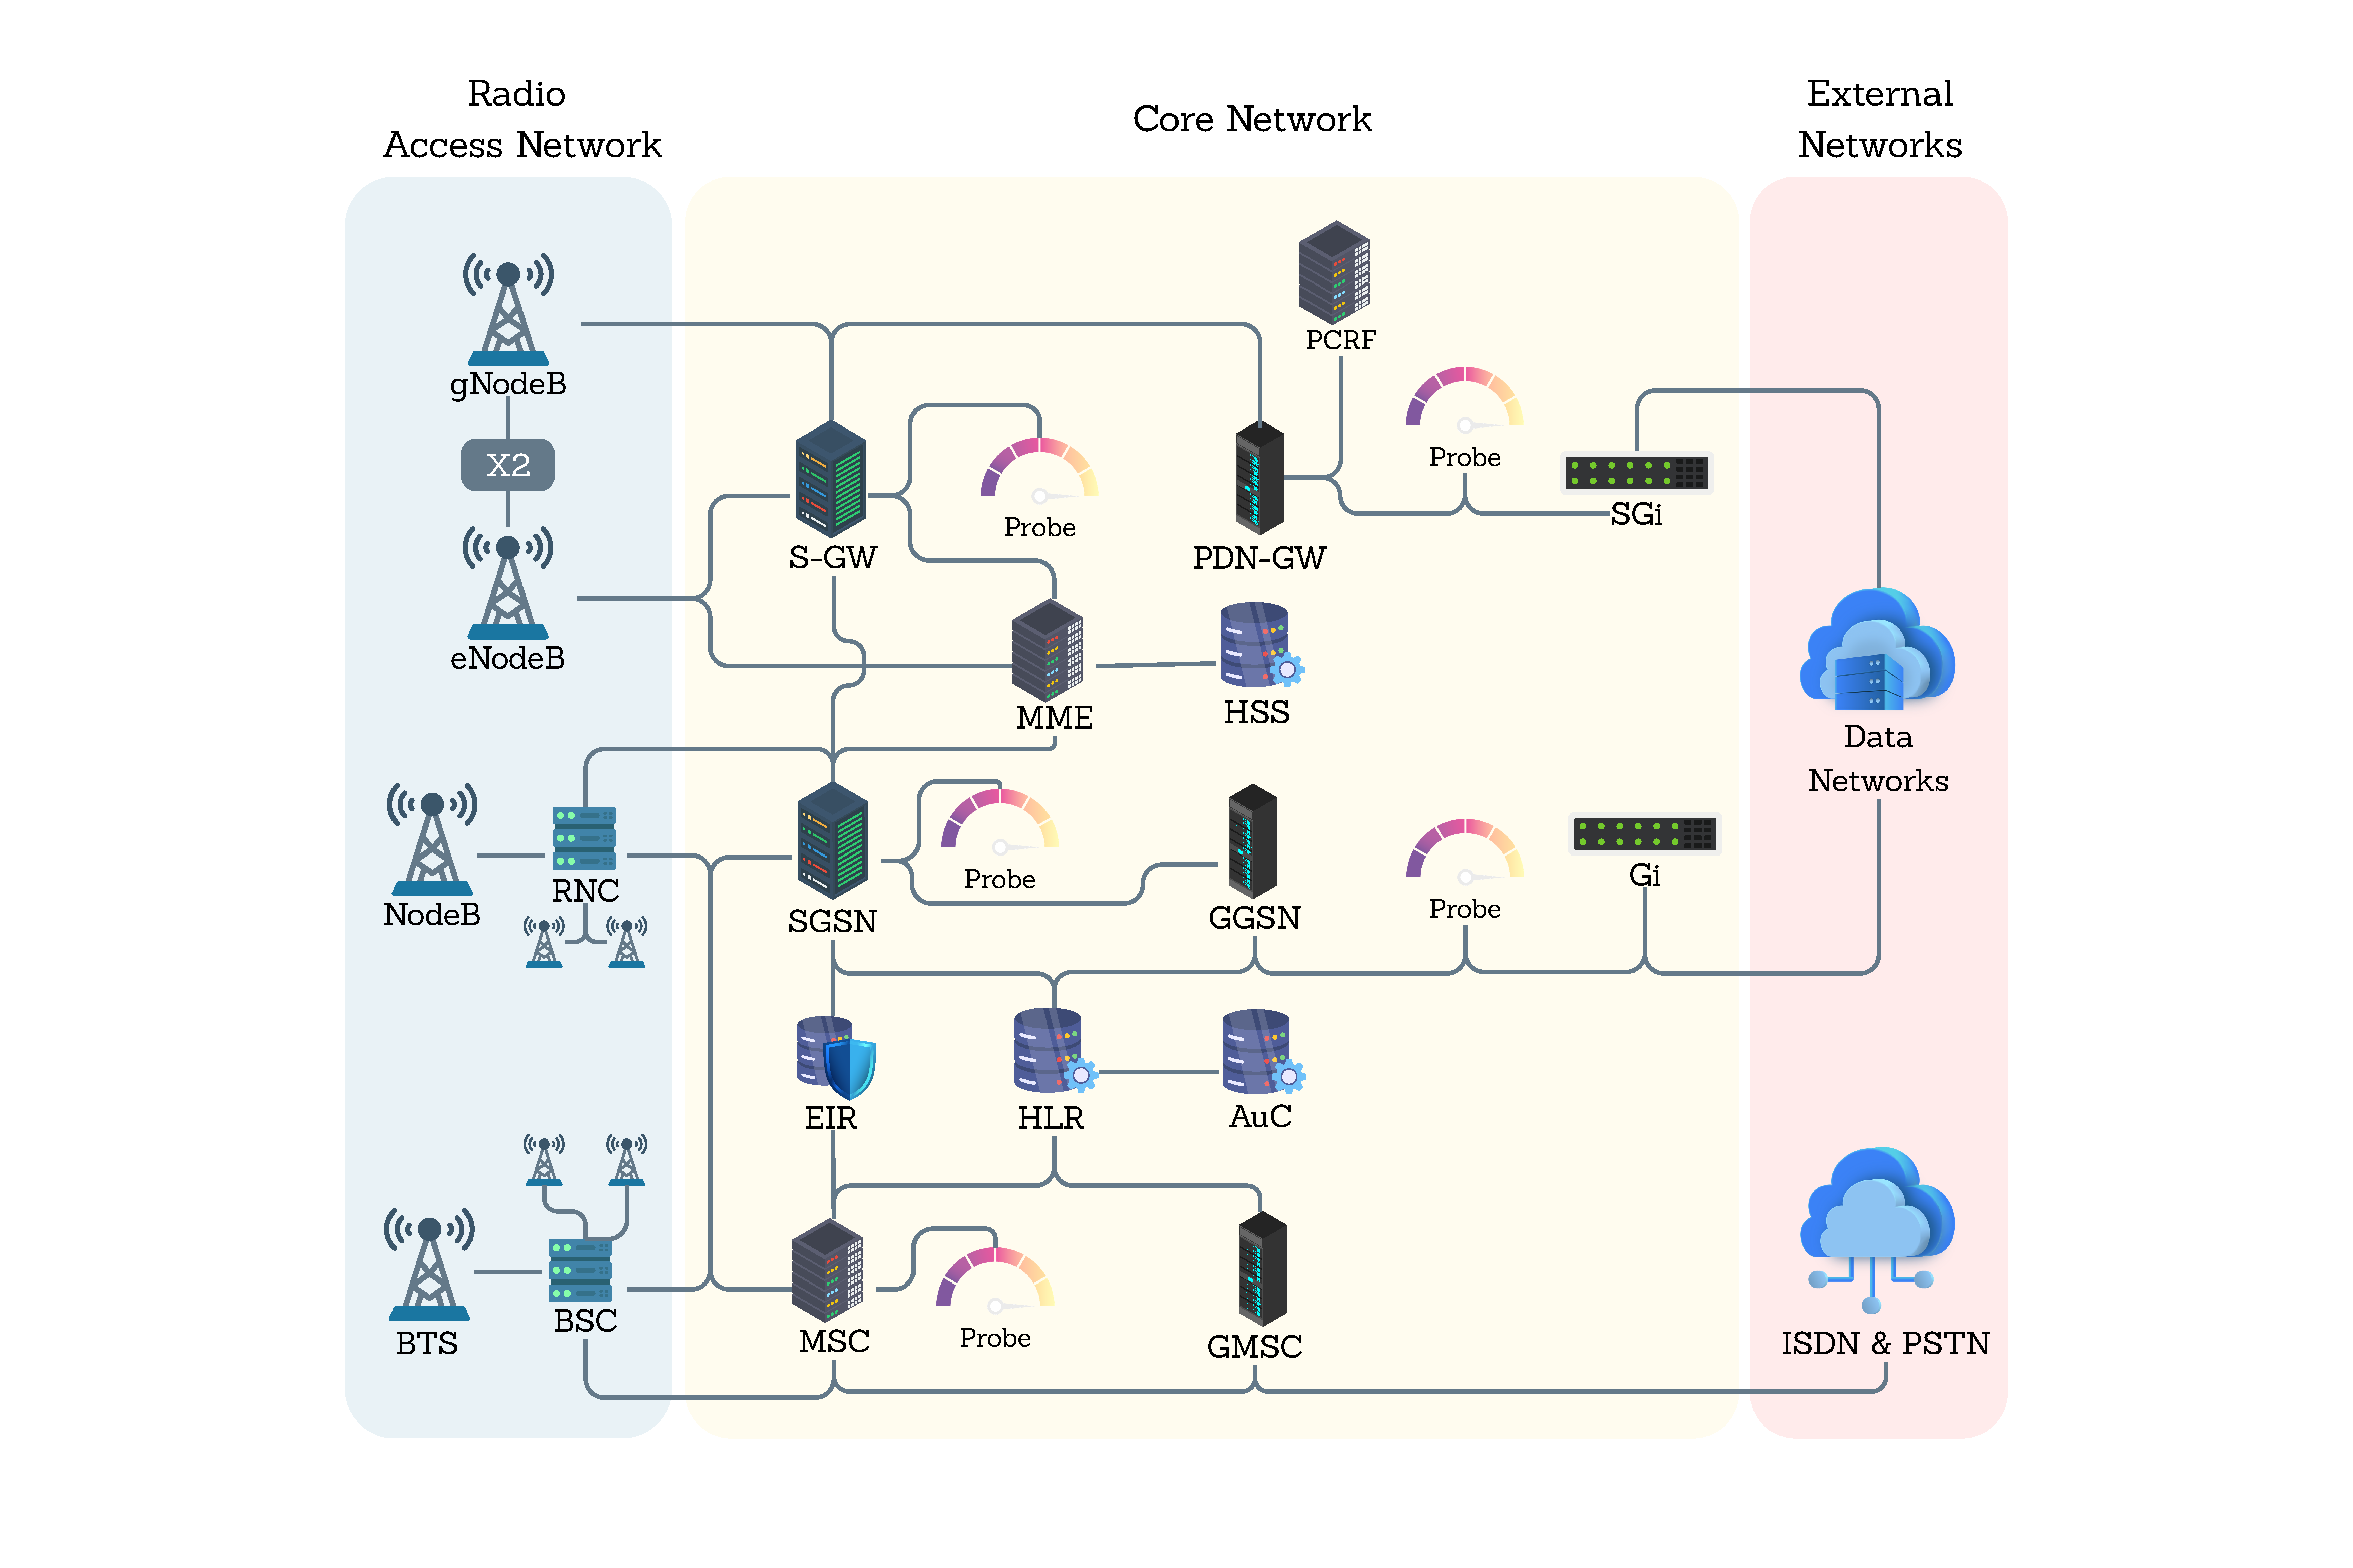
\includegraphics[width=.99\linewidth,trim={300pt 120pt 300pt 10pt},clip]{images/Appendix/mobile_network_arquitecture.pdf}
    \caption{Diagram of mobile network architecture highlighting the main nodes and interconnections across 2G, 3G, 4G, and 5G NSA generations.}
    \label{fig:network_architecture}
\end{figure}

This section describes the technical collection process for the mobile service measurements.
Figure~\ref{fig:network_architecture} provides a simplified view of the target mobile network architecture, illustrating the evolution and integration of technologies from 2G to 5G \ac{NSA} as well as the probe deployment strategy adopted by the \ac{MNO}. 
The architecture comprises the \ac{RAN}, providing wireless connectivity to the end users, and the \ac{CN}, managing mobility, authentication, and data routing. Traffic destined for external networks traverses gateway nodes that interface with public data networks, primarily the Internet. Passive measurement probes are deployed by the \ac{MNO} at two critical locations: at gateway interfaces (\ac{Gi}/\ac{SGi}) to capture traffic flows, and at signaling interfaces (S1) to capture control-plane events, enabling comprehensive monitoring of network performance and user behavior.

In \ac{LTE}, mobile networks adopt an all-IP architecture, integrating all communication into packet-switched domains. This also centralizes metadata collection at key network interfaces. Therefore, the \ac{S-GW} acts as a mobility anchor, routing data between base stations (\ac{eNodeB}) and external networks, maintaining metadata on handovers, session management, and data usage. The \ac{PDN-GW} connects mobile users to external IP networks and collects detailed metadata on traffic flows. Probes deployed at the \ac{SGi} interface between the \ac{PDN-GW} and external networks capture all data exchange, categorizing traffic by application type and providing comprehensive insights into service demand and network load.

Control-plane metadata is collected by probes at the S1 interface connecting base stations to the \ac{MME}. These probes capture signaling events related to user authentication, mobility events, and paging requests.
The collected \ac{NSD} tracks attach and detach procedures, tracking area updates, and handovers. This signaling data enables precise attribution of traffic flows to serving base stations and provides insights into user mobility patterns, essential for both network optimization and research applications.

As far as the 5G portion of the network is concerned, that is only relevant for the 2024 elections since no 5G service was active in 2019. Also, the \ac{MNO} only ran 5G in \ac{NSA} configuration in 2024, as \ac{SA} commercial services were launched only in early 2025.
Therefore, 5G traffic flows in 2024 through existing LTE core network infrastructure, which lets the same passive probe deployment capture 5G \ac{gNodeB} demands.

As expected, the network deployment also evolved between the two campaigns, growing from roughly $17{,}600$ base-station sites in 2019 to about $25{,}900$ in 2024, alongside the introduction of 5G \ac{NSA}, with an increase of around $3{,}000$ new sites in the target communes.
A denser deployment affects only the absolute traffic volume captured at each site, with no impact on our analysis.
Our per-site traffic volumes are redistributed at the commune level (see Figure~\ref{fig:voronoi_interpolation}), which is the spatial granularity of our analysis; the addition of new sites therefore translates to more sites contributing to the same commune relative to 2019, changing the absolute traffic volume attributed to each commune.
However, the \ac{SRCA} normalization is per election and at the commune level, and higher or lower absolute traffic volumes at a commune are transformed into relative, per-election values that do not propagate across campaigns.

To accurately measure individual mobile services, proprietary \ac{DPI} classifiers run on the gateway probes, associating traffic flows with specific applications (\eg YouTube, WhatsApp, Facebook) based on packet headers, payload signatures, and behavioral patterns. These three families correspond, respectively, to header-based features (such as the Server Name Indication exposed in the TLS handshake), signature matching, and flow-level heuristics, which is what allows classification to operate on largely encrypted traffic. These classifiers enable granular analysis of network traffic, allowing detailed understanding of per-service demand. The resulting metadata consists of aggregated traffic volumes recorded at each antenna over time, accompanied by geolocation information.
Beyond this description, the classifiers are the operator's production \ac{DPI} systems, and their internal methodology and per-service ground-truth accuracy are not disclosable under the commercial-sensitivity and \ac{NDA} terms that govern the data. 
Our per-app measurements therefore rely on the classifiers attributing traffic correctly, and we cannot independently validate that accuracy. 
We note, however, that these are the same classifiers the operator runs in production at national scale, a performance bar we consider well beyond what our aggregate, commune-level analysis requires.

To situate our measurements within the broader evolution of mobile consumption, we recall that global mobile data traffic grew from $38$ to $157$~EB per month between 2019 and 2024, with video rising from $63\%$ to $74\%$ of the total and average data per smartphone in Western Europe more than doubling to $23$~GB per month~\cite{ericsson_mobility_report_2019,ericsson_mobility_report_2024}. Our data reflect this expansion: the set of tracked services grew from 22 in 2019 to 27 in 2024, as platforms such as TikTok and Disney+ gained prominence (Table~\ref{tab:dataset}). Because the operator's classifiers and the absolute traffic volumes are not directly comparable across the two campaigns, we do not contrast raw demands across years; instead, we characterize each service through its commune-level \ac{SRCA} (Section~\ref{sec:data-scale}). Appendix~\ref{app:srca} illustrates the resulting spatial consumption patterns across both elections for a representative service (Figure~\ref{fig:city-instagram-srca}), and Section~\ref{sec:results-coefficient} quantifies how the per-service associations with vote shift between 2019 and 2024.

\section{Data and Code Availability}
\label{app:data-availability}


To allow reproducibility, the aggregated data and code used in this study are available in a public GitHub repository\footnote{\href{https://github.com/nds-group/digital-consumption-political-alignment-france}{https://github.com/nds-group/digital-consumption-political-alignment-france}}, with the exception of the raw mobile traffic data, which are subject to a non-disclosure agreement (\ac{NDA}) with the \ac{MNO} and cannot be redistributed.
Specifically, the repository contains:
\begin{itemize}[noitemsep, topsep=0pt, leftmargin=10pt]
    \item The electoral results obtained from the French Ministry of the Interior's open data portal~\cite{elections2019, elections2024}.
    \item The socioeconomic factors used: median income, unemployment rate, and population age structure~\cite{soc_pop_income_educ_commune}. The French public data platform does not link the specific snapshots, as these are replaced by newer versions; we therefore include our own copies, downloaded during the study period.
    \item The geospatial data, including the boundaries of each commune, their classification as urban, suburban, or rural~\cite{commune_urban}, and the city boundaries used in our spatial analysis. This information is obtained from the French public data platform~\cite{communes_boundaries}, and the specific snapshot used in this study is included in the repository.
    \item The \ac{SRCA} values for each mobile service and commune, which are the main features used in the analysis. These values are derived from the raw mobile traffic data and the aggregated traffic volumes at the commune level.
\end{itemize}

\section{Sample Representativeness}
\label{app:representativeness}

The \ac{MNO} operates under two brands: its main brand and a low-cost subsidiary, together serving approximately 22~million mobile lines (of which 3.9~million in 2019 and 4.8~million in 2024 under the low-cost brand), representing a 31.9\% share of the French mobile market, a share that remained at 31.5\% in 2024~\cite{orange2019,orange2024, orange_databook_q2_2024}.
Smartphone ownership in France is broadly uniform across income groups (72--85\%) and age cohorts (80--98\% for working-age adults;~\cite{credoc2019barometre,credoc2024barometre}).
With near-uniform penetration across the relevant demographics, the \ac{MNO}'s ${\sim}31\%$ mobile market share is unlikely to be severely skewed toward any particular socioeconomic group.
The main known residual bias is toward older age groups (smartphone ownership was 44\% for those aged 70+ in 2019, rising to 70\% by 2024; Table~\ref{tab:credoc}), a pattern expected to affect all \acp{MNO} equally.

\begin{table}[tb]
\centering
\rowcolors{2}{gray!12}{white}
\caption{Smartphone ownership in France by demographic group. Source: CREDOC, Barom\`{e}tre du num\'{e}rique~\cite{credoc2019barometre,credoc2024barometre}.}
\begin{tabular}{lrrr}
\toprule
\textbf{Dimension} & \textbf{2019} & \textbf{2024} & \textbf{Trend} \\
\midrule
Overall             & 77\% & 91\% & $+14$~pp \\
Low income          & 72\% & 90\% & $+18$~pp \\
High income         & 85\% & 95\% & $+10$~pp \\
Income gap          & 13~pp & 5~pp & halved \\
Age 18--24          & 98\% & 98\% & stable \\
Age 70+             & 44\% & 70\% & $+26$~pp \\
Rural communes      & 71\% & 84\% & $+13$~pp \\
Paris agglomeration & 83\% & 95\% & $+12$~pp \\
\bottomrule
\end{tabular}
\label{tab:credoc}
\end{table}


Figure~\ref{fig:srca-cities} illustrates what the urban and suburban commune selection looks like at intra-city resolution, using as examples LinkedIn and Facebook \ac{SRCA} values in 2019. For each service, the center map shows the full set of selected communes across metropolitan France, while the surrounding panels zoom into four metropolitan areas, revealing commune-level heterogeneity within each city. 
The two services display distinct but coherent spatial signatures, professional districts for LinkedIn and broad residential coverage for Facebook, confirming both the spatial resolution of the dataset and that service-level demand varies meaningfully within the selected communes.

\begin{figure*}[tb]
\centering
% --- LinkedIn (left half) ---
\begin{minipage}[c]{0.49\textwidth}
  \centering
  \begin{minipage}[c]{0.18\linewidth}
    \centering
    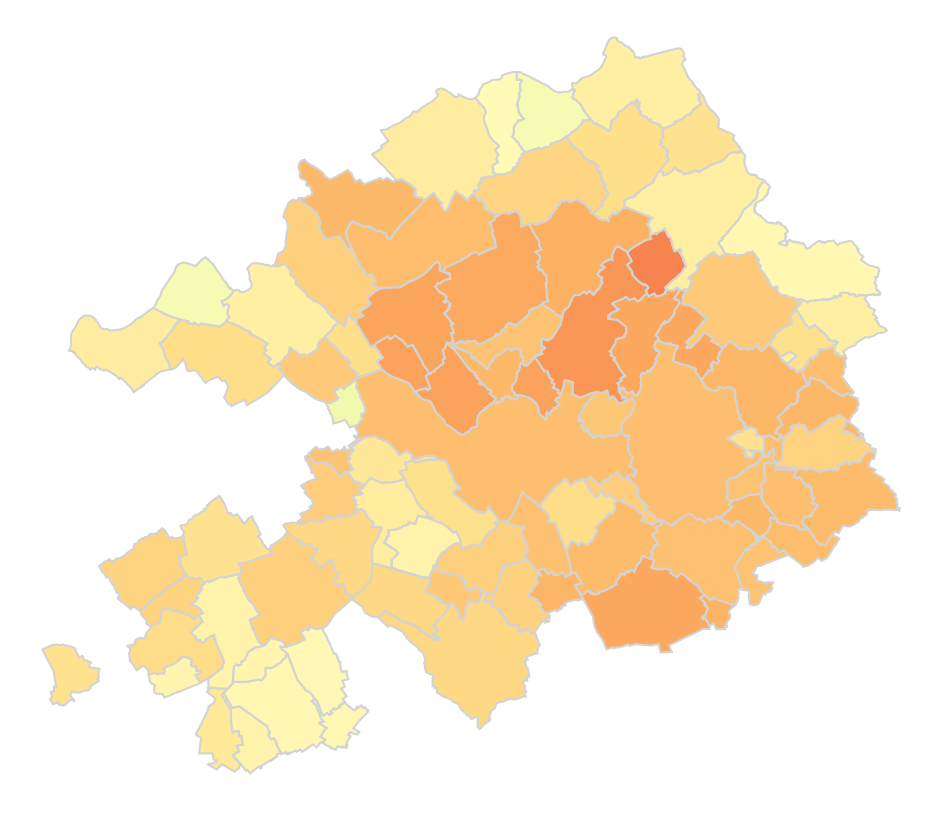
\includegraphics[width=\linewidth]{images/spatial_correlation/maps/2019/LinkedIn_srca/LinkedIn_srca_lille_urban_suburban.pdf}\\
    {\scriptsize Lille}\\[4pt]
    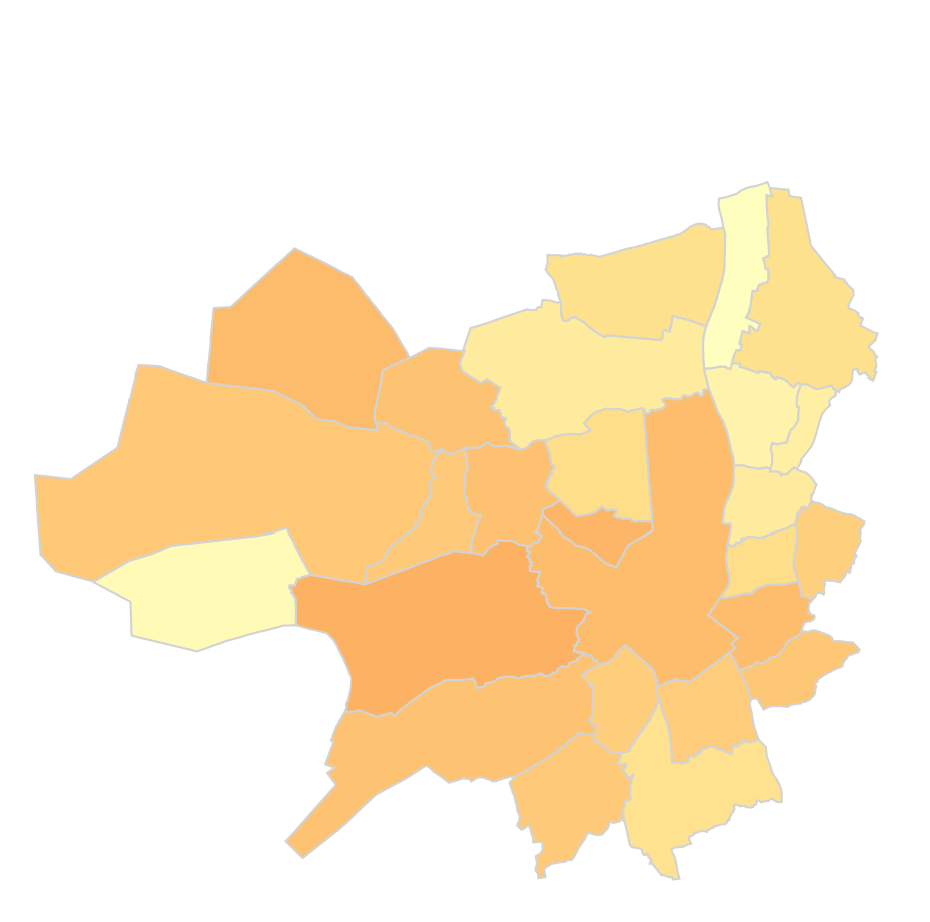
\includegraphics[width=\linewidth]{images/spatial_correlation/maps/2019/LinkedIn_srca/LinkedIn_srca_bordeaux_urban_suburban.pdf}\\
    {\scriptsize Bordeaux}
  \end{minipage}%
  \hfill%
  \begin{minipage}[c]{0.6\linewidth}
    \centering
    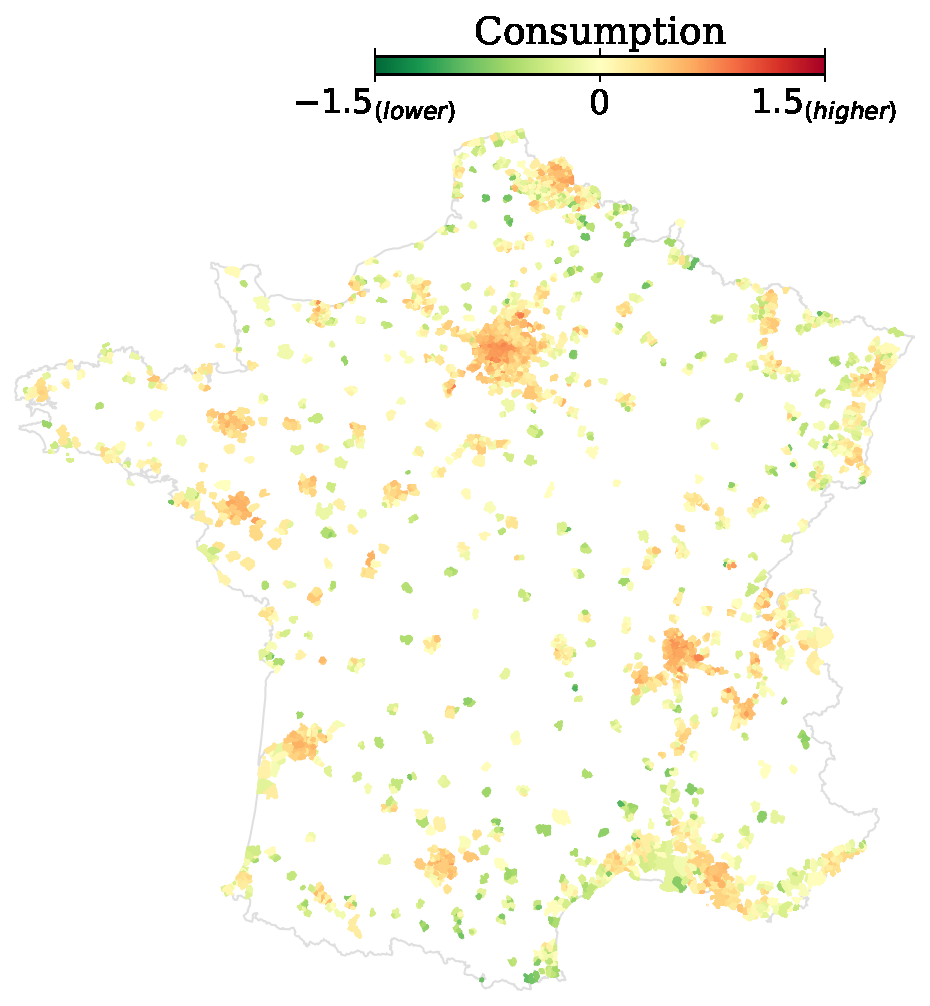
\includegraphics[width=\linewidth]{images/spatial_correlation/maps/2019/LinkedIn_srca/LinkedIn_srca_urban_suburban.pdf}
  \end{minipage}%
  \hfill%
  \begin{minipage}[c]{0.18\linewidth}
    \centering
    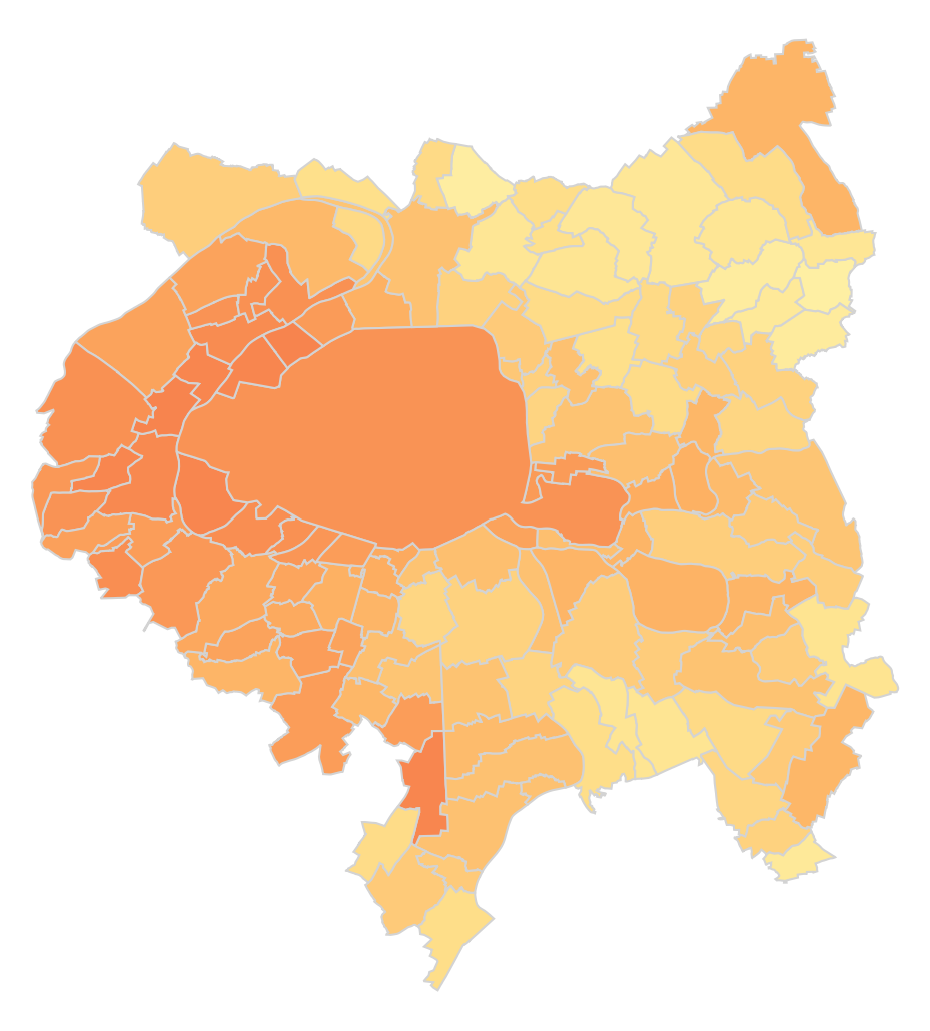
\includegraphics[width=\linewidth]{images/spatial_correlation/maps/2019/LinkedIn_srca/LinkedIn_srca_paris_urban_suburban.pdf}\\
    {\scriptsize Paris}\\[4pt]
    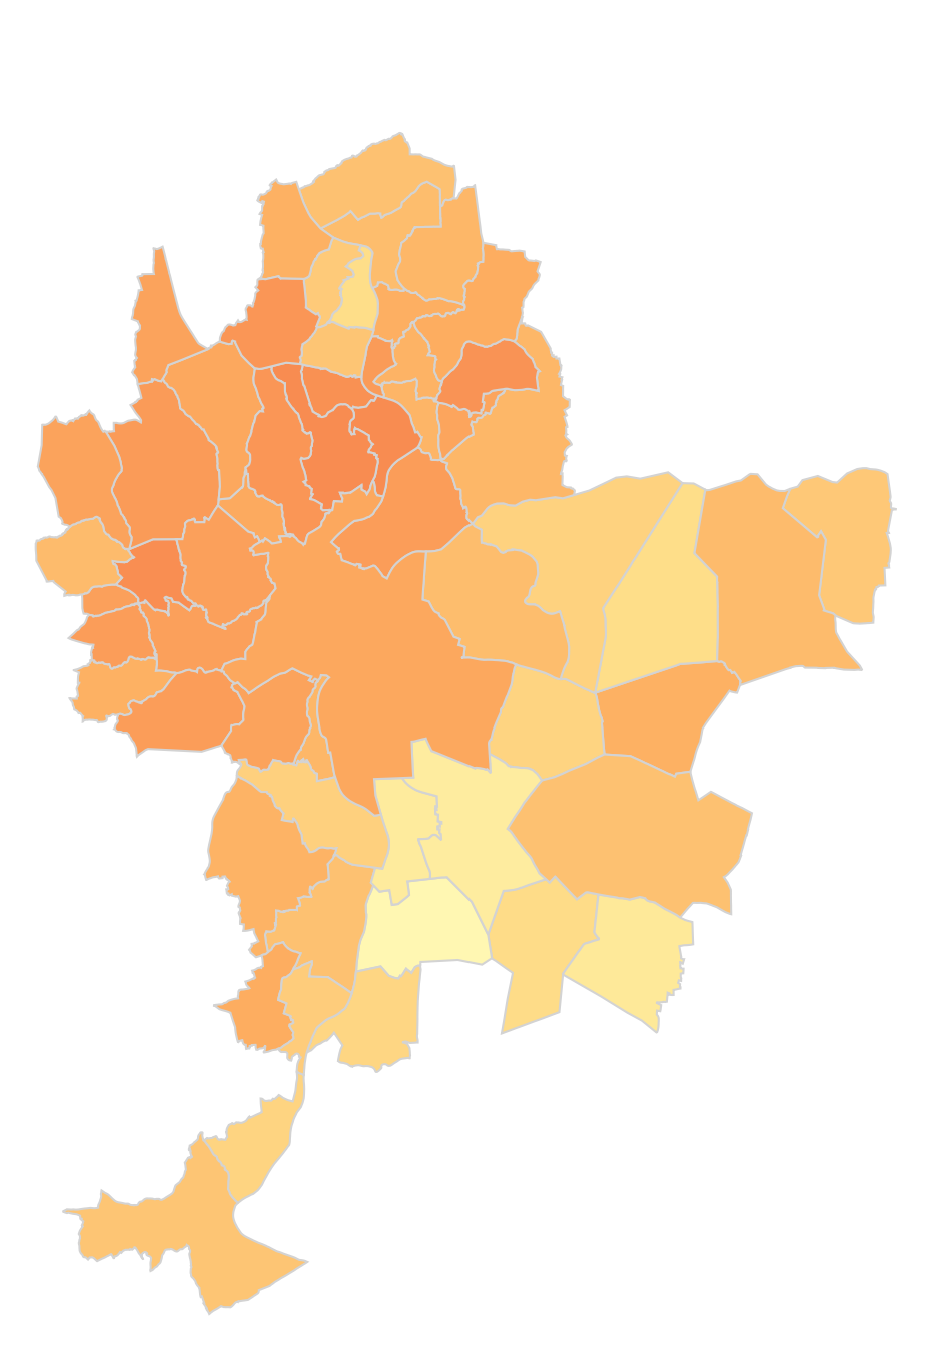
\includegraphics[width=\linewidth]{images/spatial_correlation/maps/2019/LinkedIn_srca/LinkedIn_srca_lyon_urban_suburban.pdf}\\
    {\scriptsize Lyon}
  \end{minipage}\\[4pt]
  {\small (a) LinkedIn}
\end{minipage}
\hfill
% --- Facebook (right half) ---
\begin{minipage}[c]{0.49\textwidth}
  \centering
  \begin{minipage}[c]{0.18\linewidth}
    \centering
    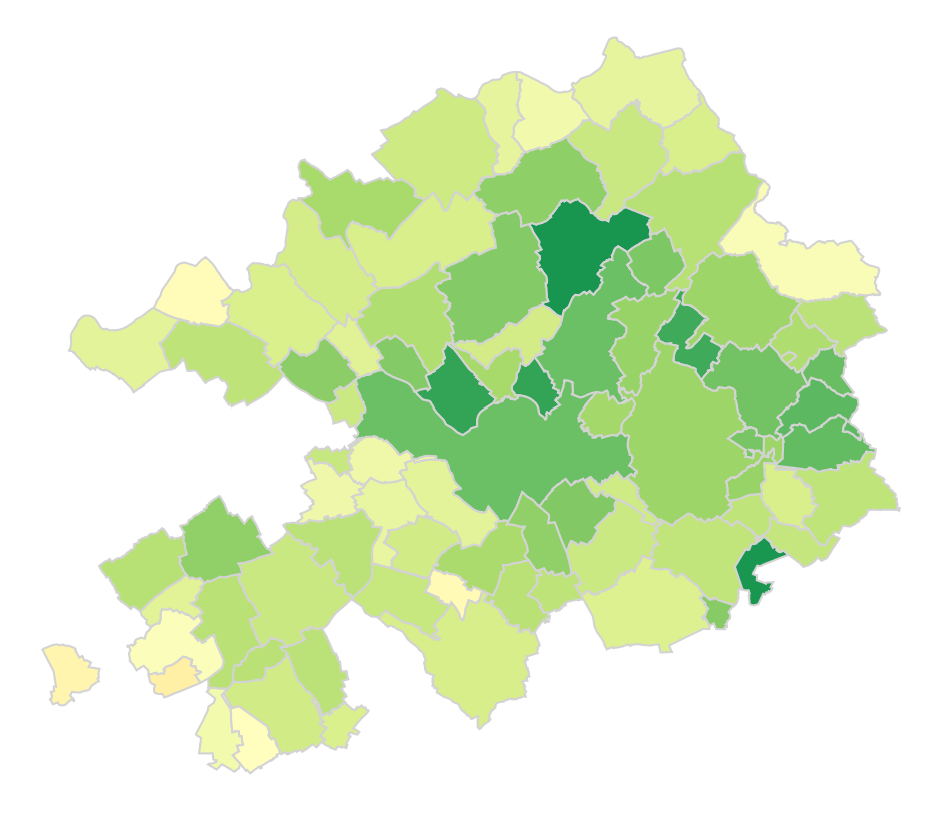
\includegraphics[width=\linewidth]{images/spatial_correlation/maps/2019/Facebook_srca/Facebook_srca_lille_urban_suburban.pdf}\\
    {\scriptsize Lille}\\[4pt]
    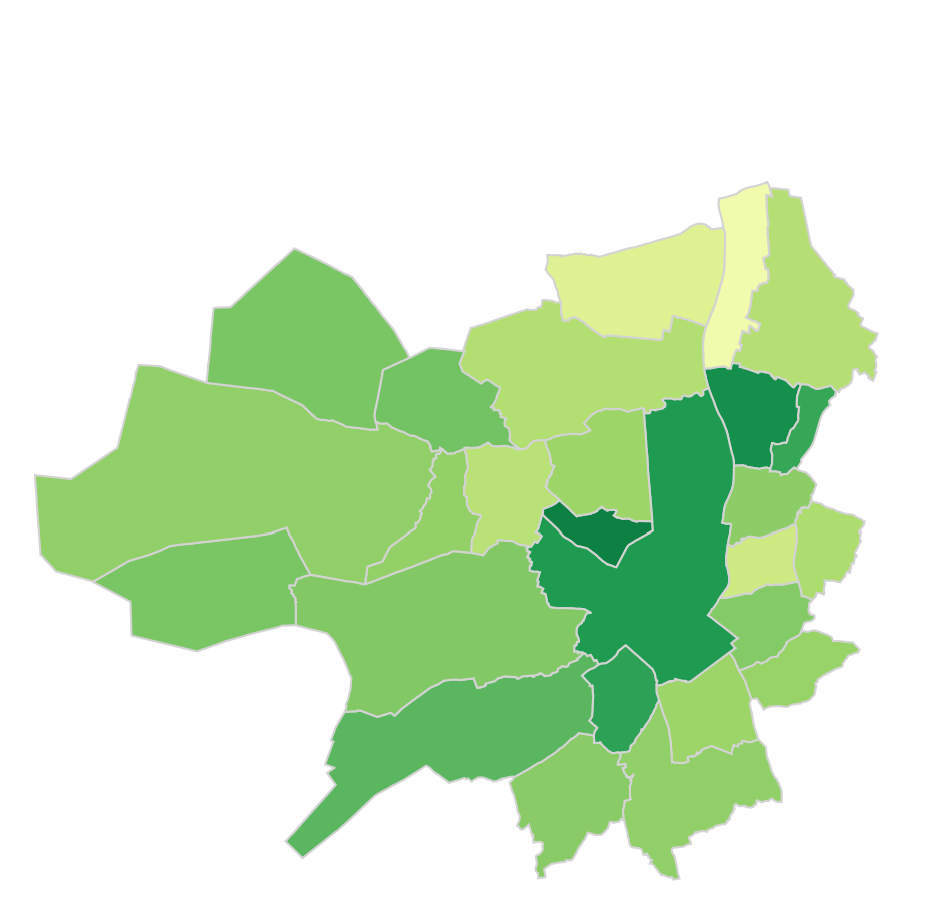
\includegraphics[width=\linewidth]{images/spatial_correlation/maps/2019/Facebook_srca/Facebook_srca_bordeaux_urban_suburban.pdf}\\
    {\scriptsize Bordeaux}
  \end{minipage}%
  \hfill%
  \begin{minipage}[c]{0.6\linewidth}
    \centering
    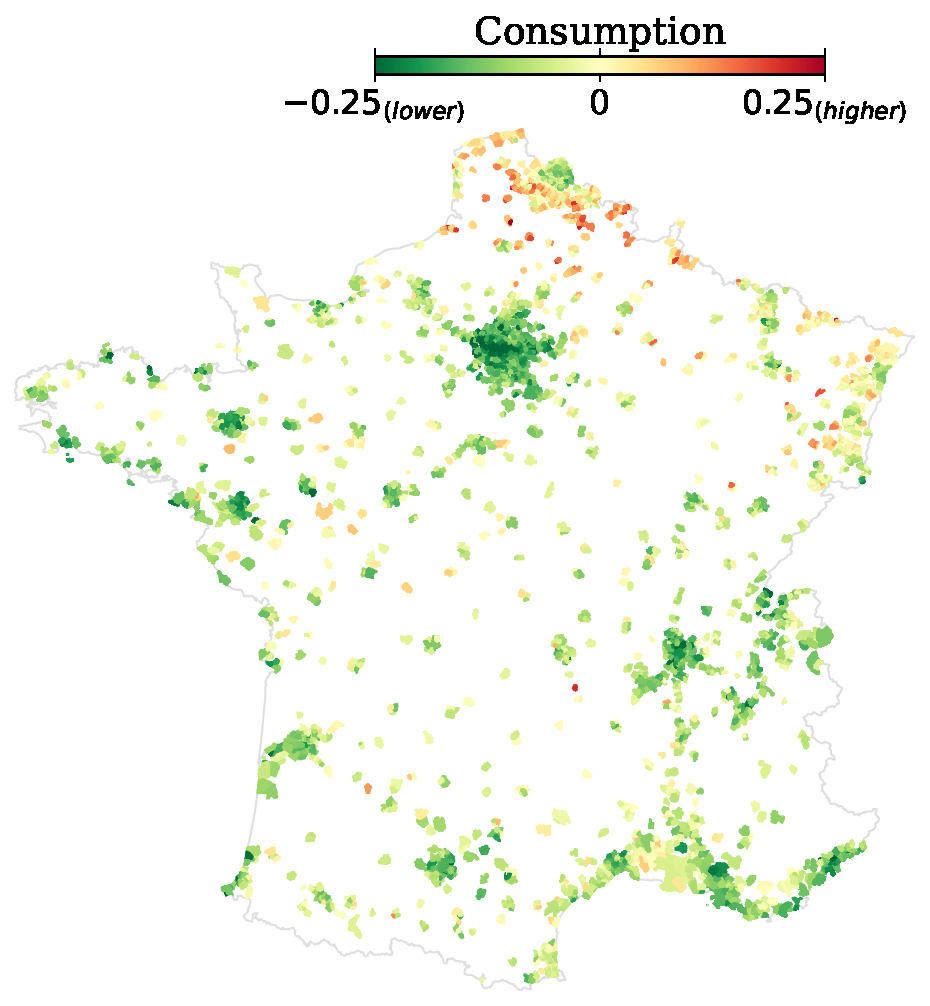
\includegraphics[width=\linewidth]{images/spatial_correlation/maps/2019/Facebook_srca/Facebook_srca_urban_suburban.pdf}
  \end{minipage}%
  \hfill%
  \begin{minipage}[c]{0.18\linewidth}
    \centering
    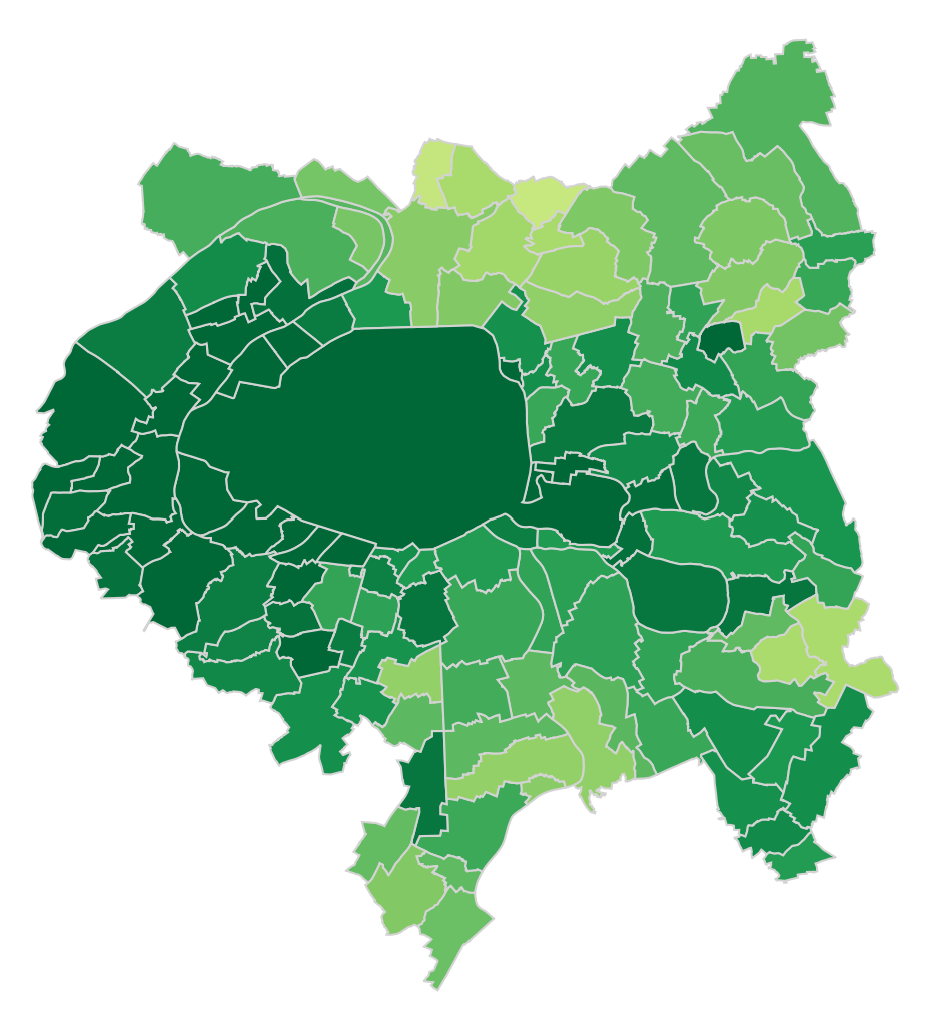
\includegraphics[width=\linewidth]{images/spatial_correlation/maps/2019/Facebook_srca/Facebook_srca_paris_urban_suburban.pdf}\\
    {\scriptsize Paris}\\[4pt]
    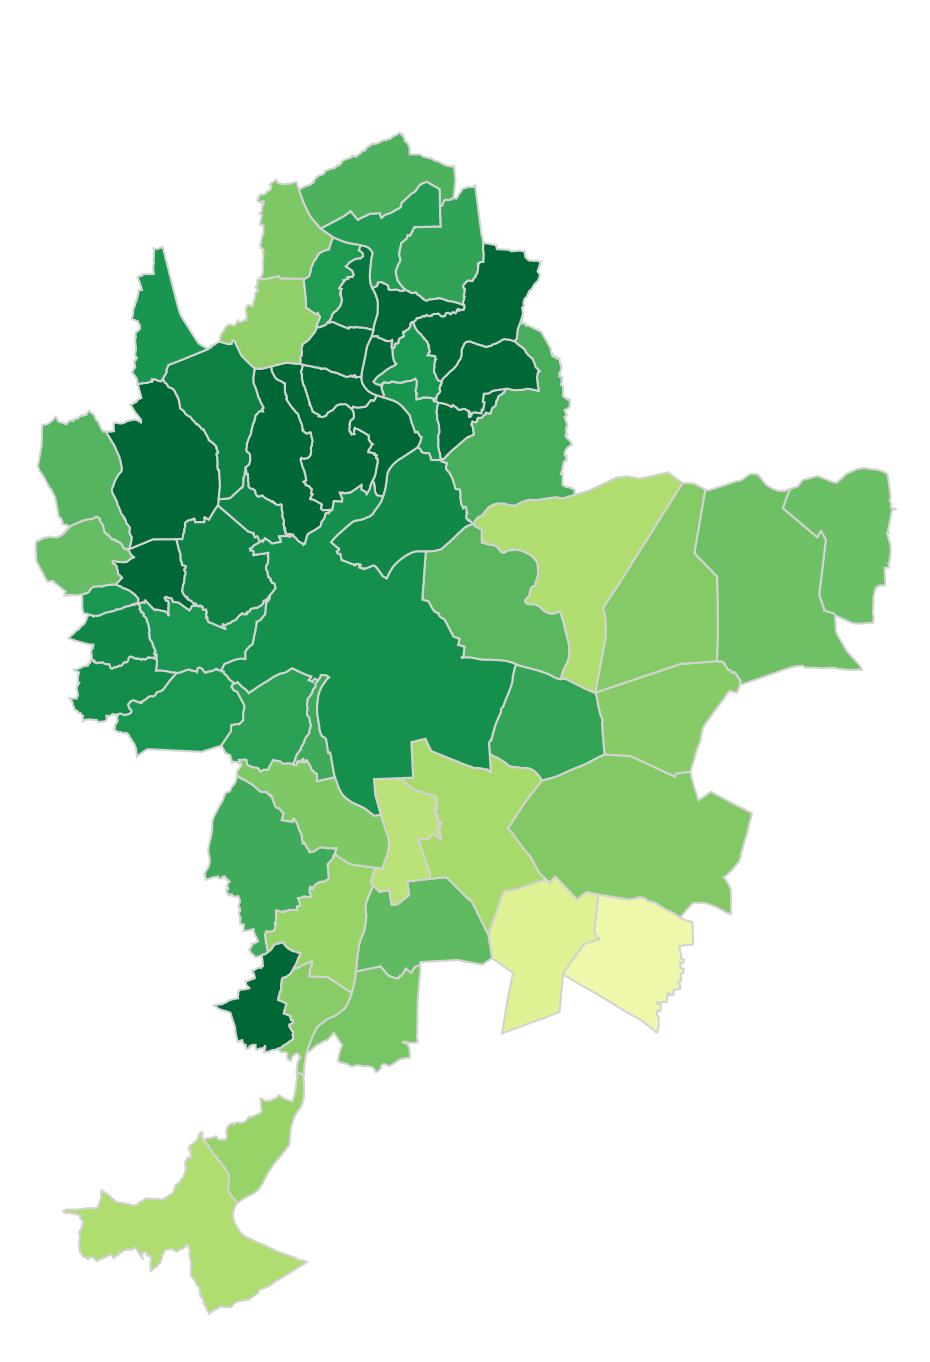
\includegraphics[width=\linewidth]{images/spatial_correlation/maps/2019/Facebook_srca/Facebook_srca_lyon_urban_suburban.pdf}\\
    {\scriptsize Lyon}
  \end{minipage}\\[4pt]
  {\small (b) Facebook}
\end{minipage}
\caption{\ac{SRCA} of (a) LinkedIn and (b) Facebook across urban and suburban communes (center map of each panel) and four metropolitan areas (2019). Commune boundaries are visible at city scale, confirming the spatial resolution of the dataset; the two services exhibit distinct spatial signatures within the same selected communes.
\label{fig:srca-cities}}
\end{figure*}

\section{Representativeness of \ac{SRCA}}
\label{app:srca}

Figure~\ref{fig:raw_rca_srca} illustrates the effect of transforming from Raw traffic distribution for Facebook and WhatsApp traffic to \ac{RCA} and to \ac{SRCA}.
The raw traffic map (left) conflates two confounds: $i)$ the intrinsic byte footprint of the service and $ii)$ the population density of the commune, making high-traffic communes indistinguishable from communes with genuine relative preference for the service. 
Raw values are shown in anonymized units (multiplied by a constant $10^{k}$ per the \ac{NDA}).
The \ac{RCA} map (center) normalizes away both confounds simultaneously: the numerator removes the service's national byte footprint and the denominator removes the commune's total traffic, revealing genuine spatial heterogeneity in service preference.
The \ac{SRCA} map (right) applies the symmetric rescaling to $(-1, 1)$, removing the asymmetry between advantage and disadvantage in raw \ac{RCA} values and making the index comparable across services with very different traffic volumes.

\begin{figure*}[tb]
\raggedleft
\subfloat{
\includegraphics[width=0.4\textwidth]{images/consolidation/RCA/legend.pdf}}

\setcounter{subfigure}{0}
\centering
\subfloat[Raw traffic]{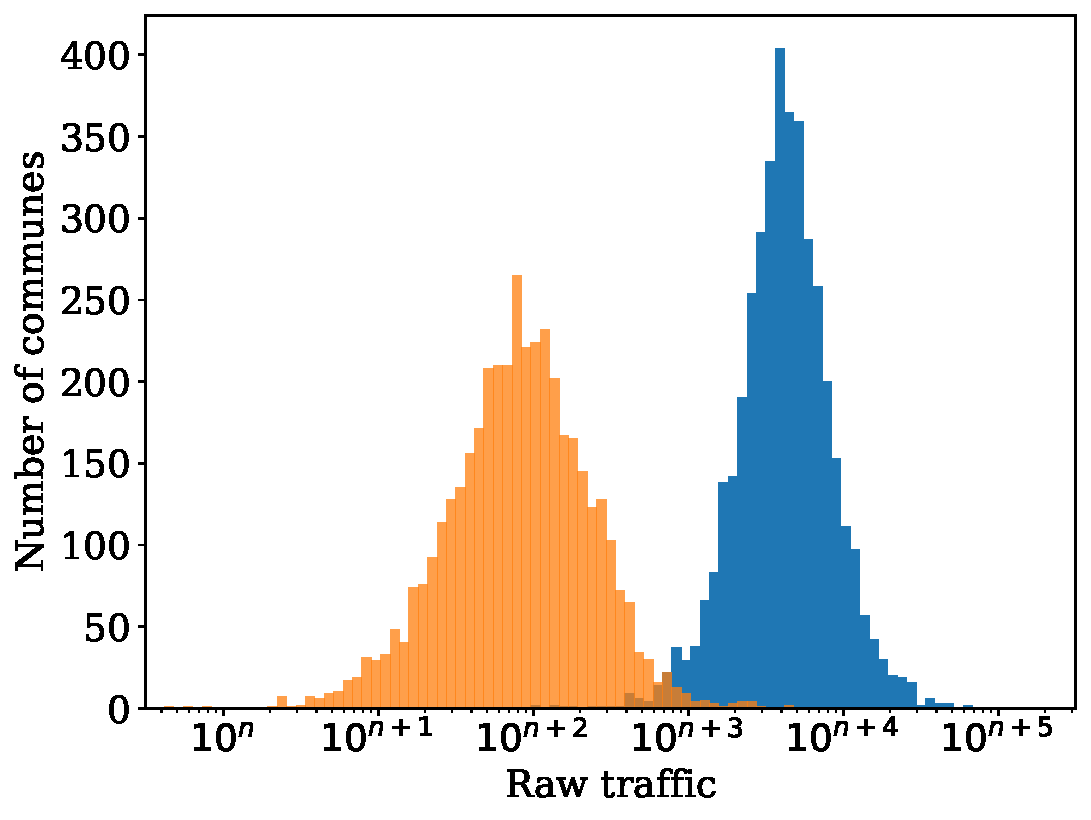
\includegraphics[width=0.3\textwidth,trim=0 25pt 0 0,clip]{images/consolidation/RCA/Facebook_WhatsApp_raw_2019.pdf}}
\hfill
\subfloat[\ac{RCA}]{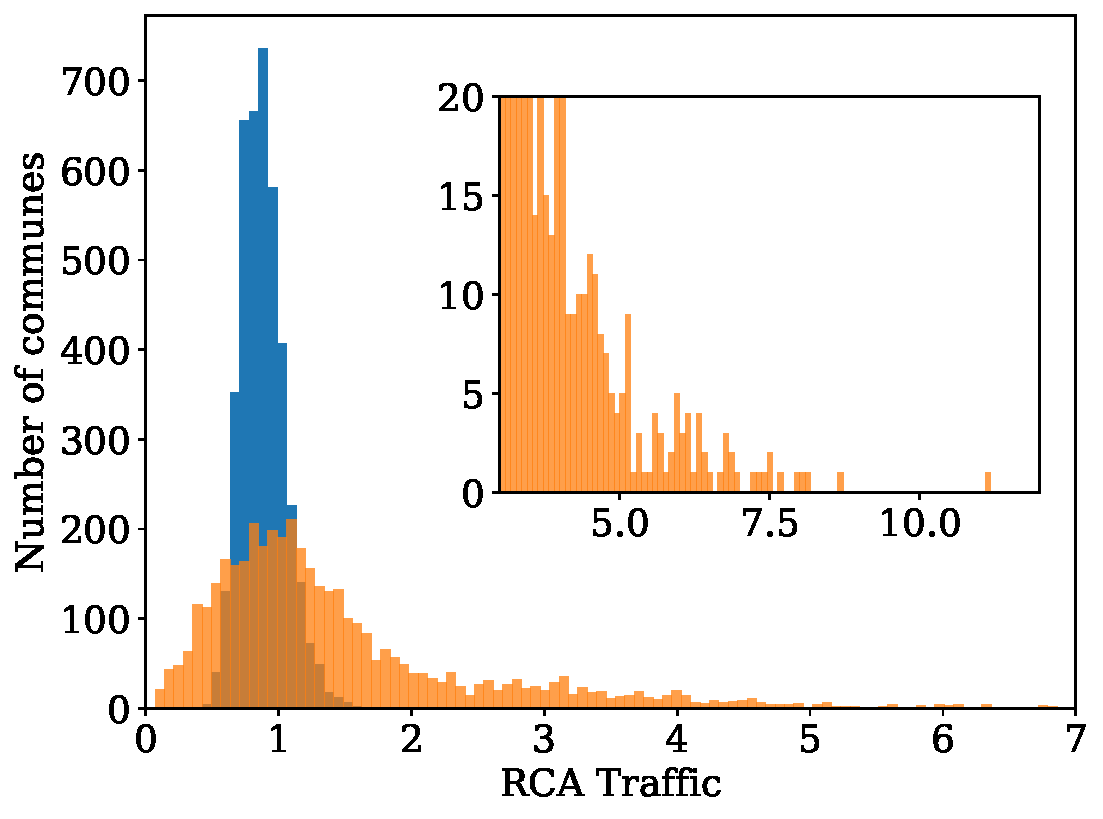
\includegraphics[width=0.3\textwidth,trim=0 25pt 0 0,clip]{images/consolidation/RCA/Facebook_WhatsApp_rca_2019.pdf}}
\hfill
\subfloat[\ac{SRCA}]{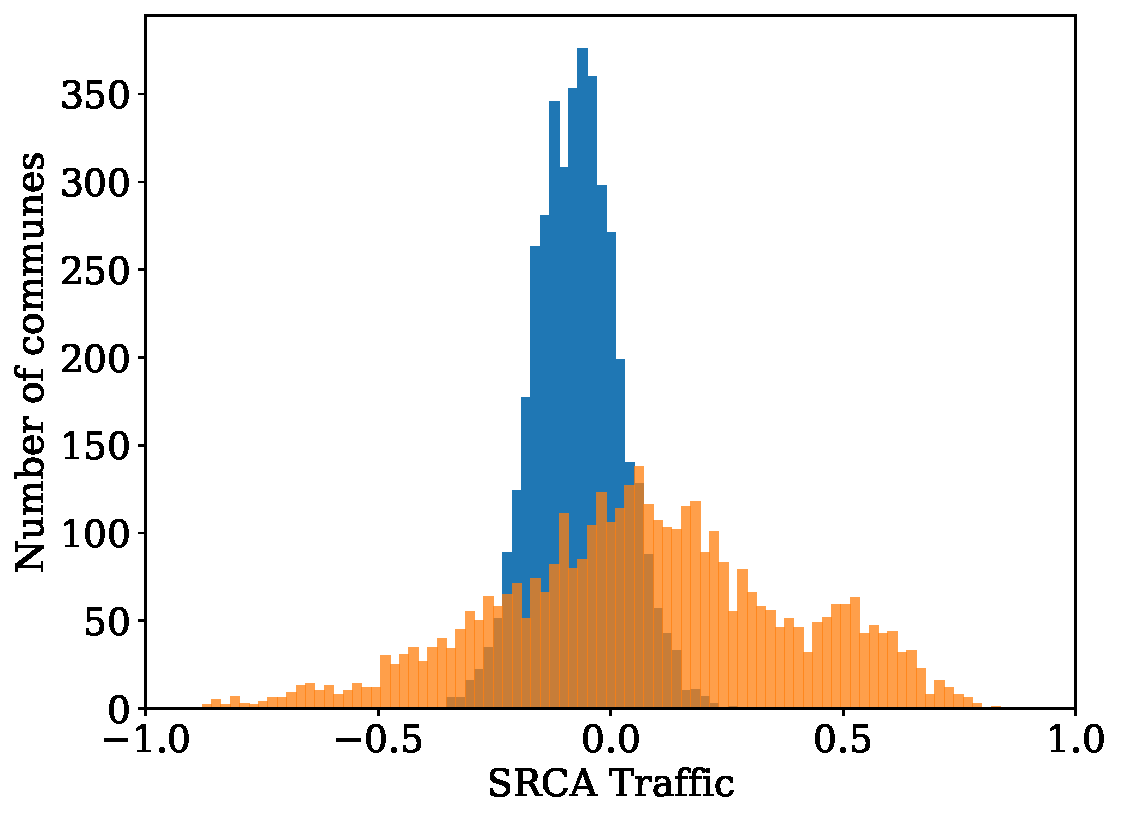
\includegraphics[width=0.3\textwidth,trim=0 25pt 0 0,clip]{images/consolidation/RCA/Facebook_WhatsApp_srca_2019.pdf}}

\caption{Effect of the Raw to \ac{RCA}  and \ac{SRCA} transformation for Facebook and WhatsApp traffic across French communes. Raw traffic (left) reflects population density more than service preference; values are in anonymized units ($\bm{\times 10^{n}}$) per the \ac{NDA}. \ac{RCA} (center) normalizes by commune size and national service share, removing both confounds. \ac{SRCA} (right) symmetrizes the index to $\bm{(-1,1)}$, enabling direct cross-service comparison.
\label{fig:raw_rca_srca}}
\end{figure*}

Figure~\ref{fig:city-instagram-srca} shows commune-level \ac{SRCA} patterns for a representative service (Instagram) across the six largest French metropolitan areas, comparing 2019 (top row) and 2024 (bottom row). Vertical comparison tracks the stability of consumption patterns across elections in a city; horizontal comparison reveals how the spatial footprint varies across cities.


\begin{figure*}[h]
\raggedleft
\subfloat{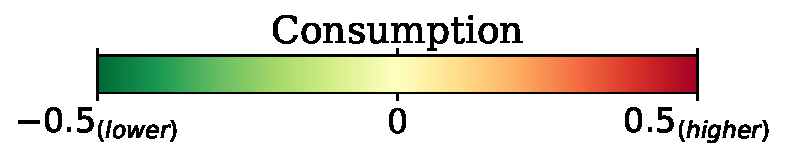
\includegraphics[width=0.2\textwidth]{images/spatial_correlation/maps/2019/Instagram_srca/Instagram_srca_urban_suburban_colorbar.pdf}}
\vspace{-5pt}

\centering

\subfloat{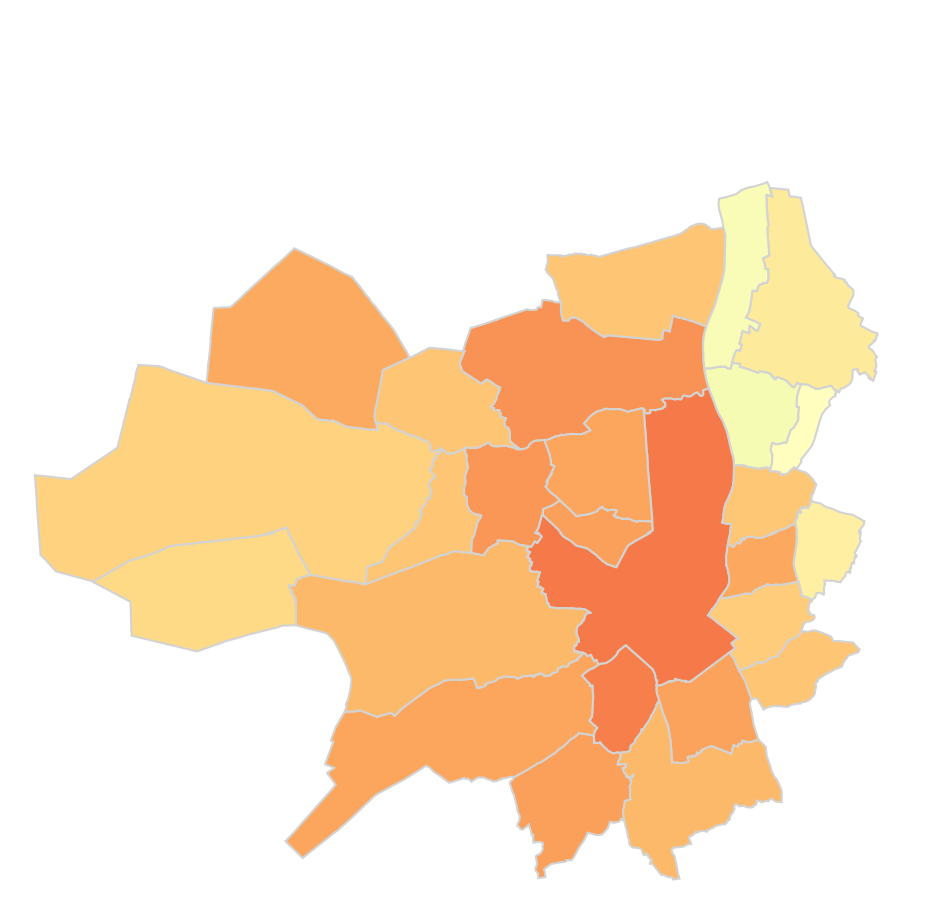
\includegraphics[width=0.14\textwidth]{images/spatial_correlation/maps/2019/Instagram_srca/Instagram_srca_bordeaux_urban_suburban.pdf}}\hfill
\subfloat{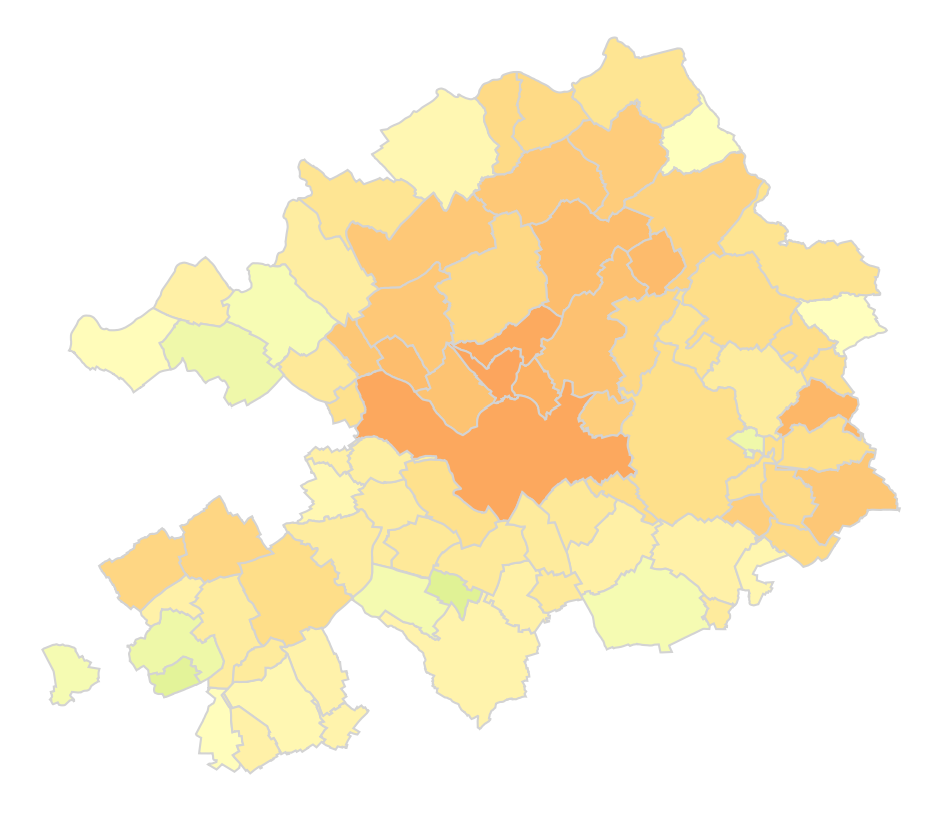
\includegraphics[width=0.155\textwidth]{images/spatial_correlation/maps/2019/Instagram_srca/Instagram_srca_lille_urban_suburban.pdf}}\hfill
\subfloat{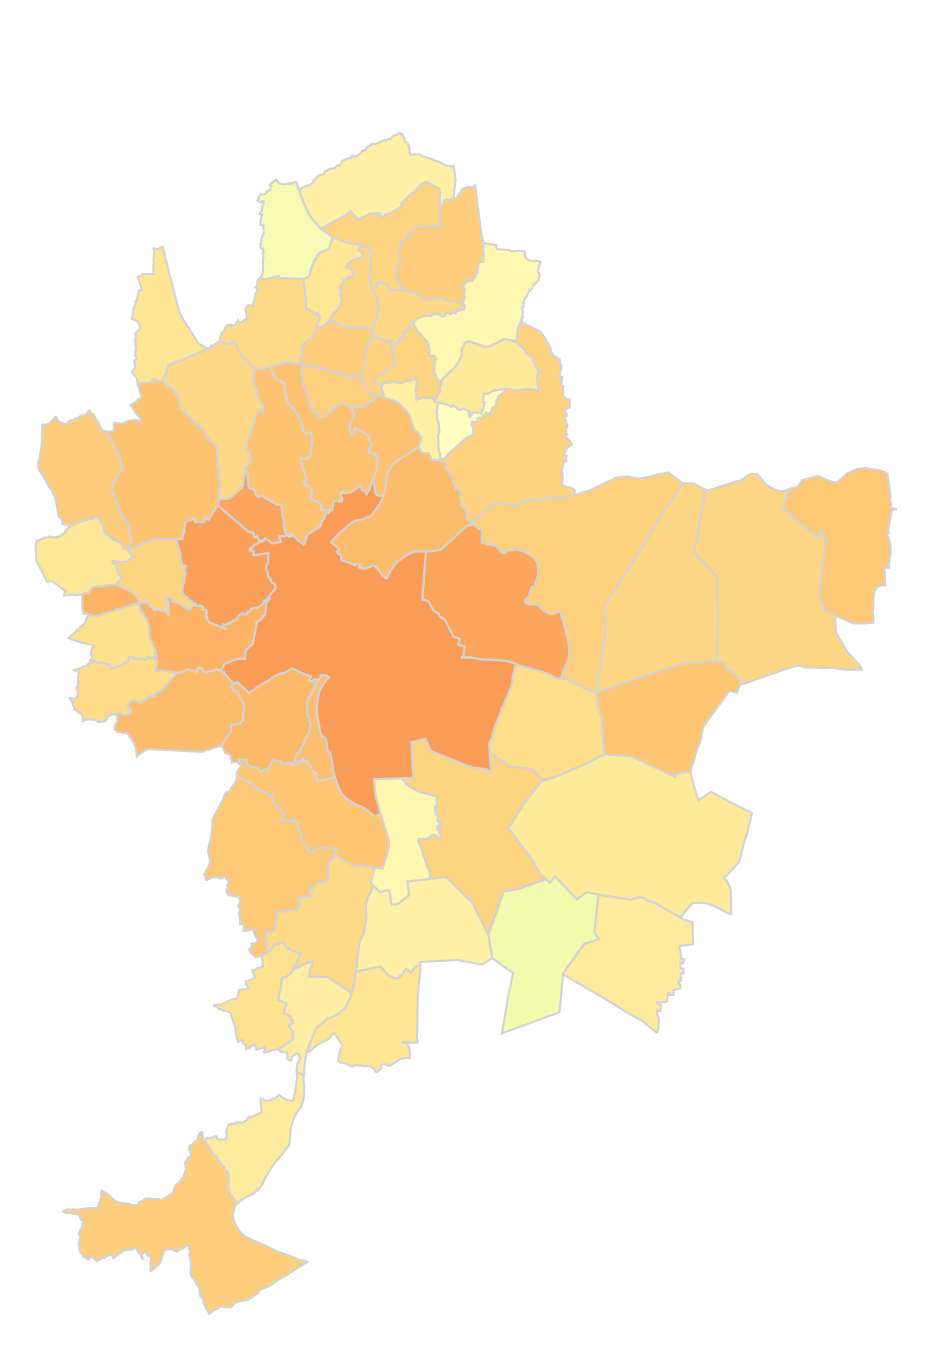
\includegraphics[height=0.18\textwidth]{images/spatial_correlation/maps/2019/Instagram_srca/Instagram_srca_lyon_urban_suburban.pdf}}\hfill
\subfloat{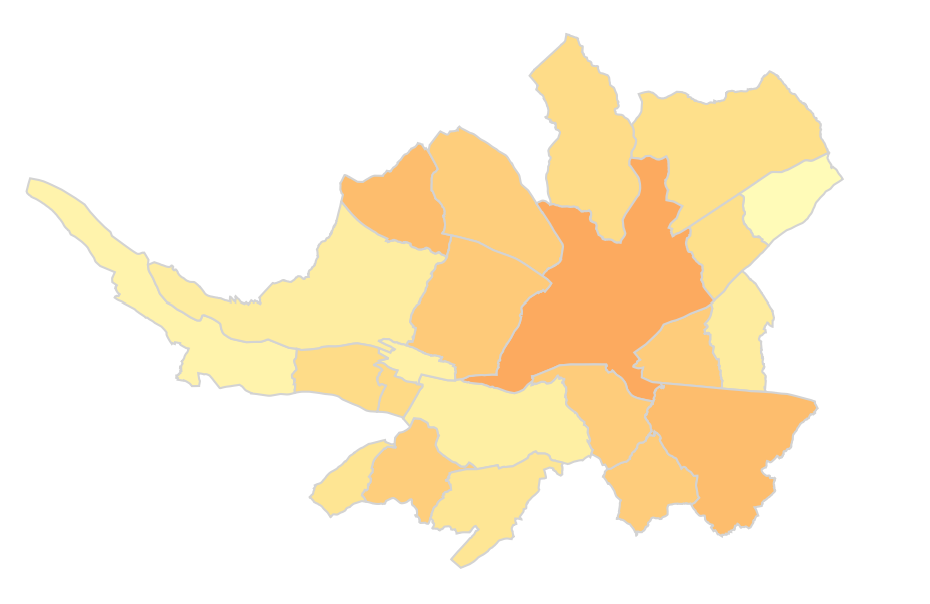
\includegraphics[height=0.11\textwidth]{images/spatial_correlation/maps/2019/Instagram_srca/Instagram_srca_nantes_urban_suburban.pdf}}\hfill
\subfloat{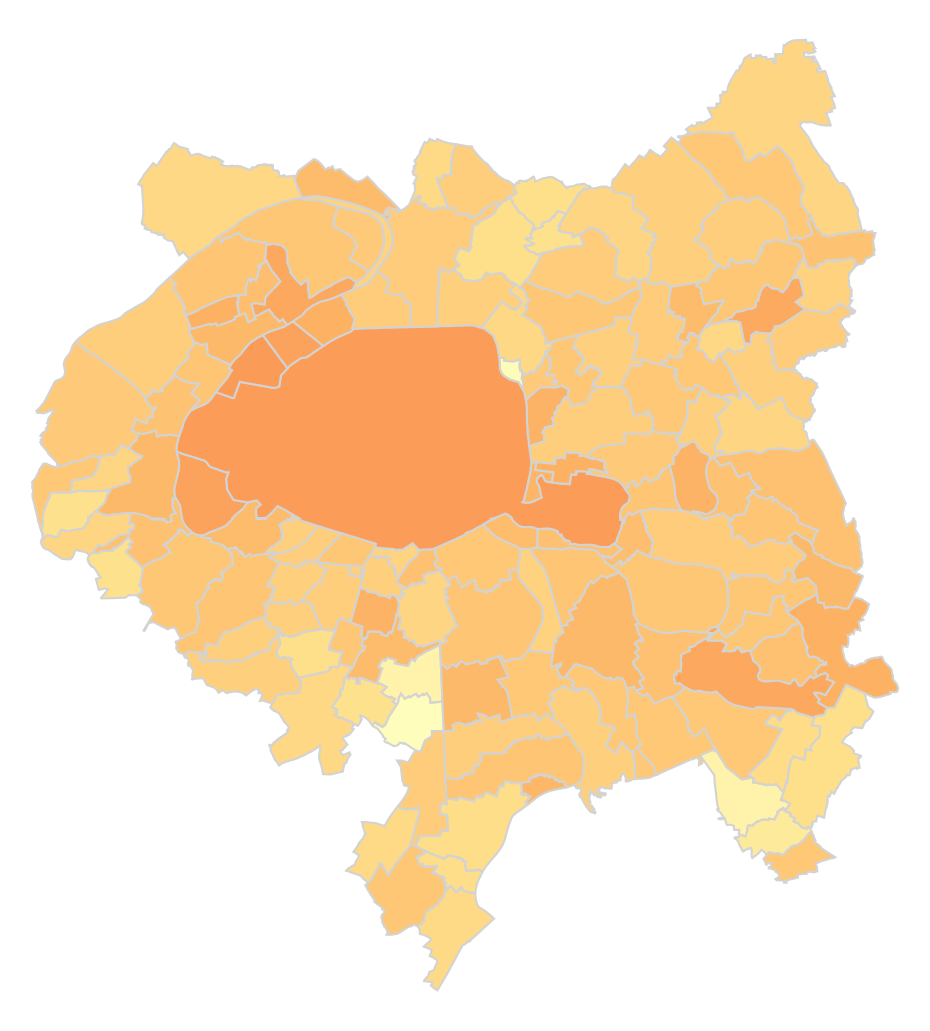
\includegraphics[width=0.14\textwidth]{images/spatial_correlation/maps/2019/Instagram_srca/Instagram_srca_paris_urban_suburban.pdf}}\hfill
\subfloat{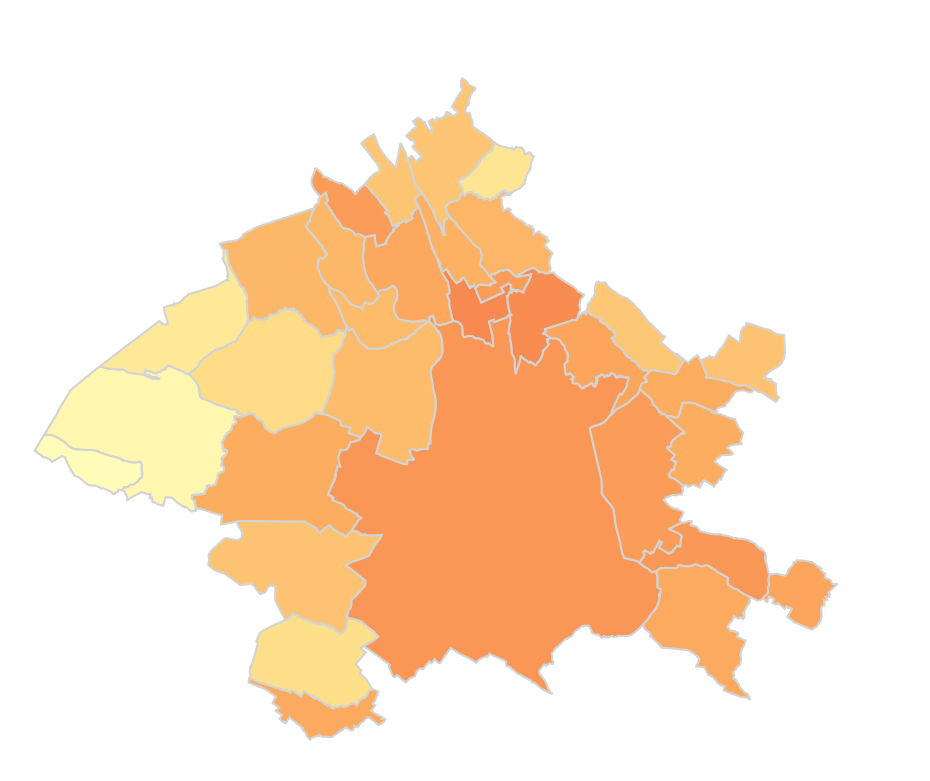
\includegraphics[width=0.155\textwidth]{images/spatial_correlation/maps/2019/Instagram_srca/Instagram_srca_toulouse_urban_suburban.pdf}}\\
\setcounter{subfigure}{0}
\subfloat[Bordeaux]{
\includegraphics[width=0.14\textwidth]{images/spatial_correlation/maps/2024/Instagram_srca/Instagram_srca_bordeaux_urban_suburban.pdf}}\hfill
\subfloat[Lille]{
\includegraphics[width=0.155\textwidth]{images/spatial_correlation/maps/2024/Instagram_srca/Instagram_srca_lille_urban_suburban.pdf}}\hfill
\subfloat[Lyon]{
\includegraphics[height=0.18\textwidth]{images/spatial_correlation/maps/2024/Instagram_srca/Instagram_srca_lyon_urban_suburban.pdf}}\hfill
\subfloat[Nantes]{
\includegraphics[height=0.11\textwidth]{images/spatial_correlation/maps/2024/Instagram_srca/Instagram_srca_nantes_urban_suburban.pdf}}\hfill
\subfloat[Paris]{
\includegraphics[width=0.14\textwidth]{images/spatial_correlation/maps/2024/Instagram_srca/Instagram_srca_paris_urban_suburban.pdf}}\hfill
\subfloat[Toulouse]{
\includegraphics[width=0.155\textwidth]{images/spatial_correlation/maps/2024/Instagram_srca/Instagram_srca_toulouse_urban_suburban.pdf}}
\caption{Instagram \ac{SRCA} across six French metropolitan areas in 2019 (top) and 2024 (bottom).
\label{fig:city-instagram-srca}}
\end{figure*}


\section{Political Science Literature}
\label{app:polisci}

Table~\ref{tab:polisci} places our work in the context of prior research on digital media and elections, comparing each study along its objective, dataset and identification strategy, coverage, and key finding.
These studies span diverse designs, from survey panels and web-tracking to field and natural experiments, and most examine a single platform, predominantly in the United States.
Where they rely on surveys, platform APIs, or single-platform traces, our study instead draws on passive, unsampled \ac{MNO} traffic spanning tens of services and two consecutive elections at commune-level granularity, offering a complementary, population-scale vantage.

\begin{table*}[p]
\centering
\vspace*{\fill}
\rotatebox{90}{%
\begin{minipage}{\textheight}
\centering
\setlength{\tabcolsep}{4pt}
\renewcommand{\arraystretch}{1.2}
\rowcolors{2}{gray!8}{white}
\begin{tabular}{>{\raggedright\arraybackslash}p{2.7cm} >{\raggedright\arraybackslash}p{3.9cm} >{\raggedright\arraybackslash}p{5.3cm} >{\raggedright\arraybackslash}p{3.6cm} >{\raggedright\arraybackslash}p{5.1cm}}
\toprule
\textbf{Study} & \textbf{Objective} & \textbf{Dataset (identification)} & \textbf{Coverage} & \textbf{Key finding} \\
\midrule
Allcott \& Gentzkow (2017)~\cite{allcott2017social}
  & Measure prevalence and persuasive effect of fake news
  & YouGov survey panel ($\sim$1{,}200) + web-traffic data + Facebook post database (observational)
  & US, 2016 Presidential
  & Fake-news exposure was widespread, but its persuasive effect on votes was limited \\
Schaub \& Morisi (2020)~\cite{schaub2020voter}
  & Test whether broadband internet causally increases populist support
  & Municipal broadband coverage + survey data (quasi-exp., IV)
  & Italy \& Germany, national elections ($\sim$2013--2018)
  & Broadband access increased populist party support \\
Guriev, Melnikov \& Zhuravskaya (2021)~\cite{guriev20213g}
  & Estimate effect of 3G expansion on confidence in government
  & Gallup World Poll + GSMA 3G coverage maps (quasi-exp., IV)
  & 116 countries, 2008--2017
  & 3G expansion reduced confidence in government \\
M{\"u}ller \& Schwarz (2021)~\cite{muller2021fanning}
  & Link right-wing Facebook activity to hate-crime incidence
  & AfD Facebook posts + German hate-crime registry + platform-outage instrument (quasi-exp., IV)
  & Germany, 2010--2017
  & Higher local Facebook activity increased hate-crime incidence \\
Melnikov (2021)~\cite{melnikov2021mobile}
  & Estimate causal effect of 3G mobile internet on political polarization
  & Gallup Daily Poll (1.76M individuals, 31{,}499 ZIP codes) + 3G rollout (quasi-exp., DiD)
  & US, 2008--2017
  & 3G mobile internet increased partisan polarization \\
Levy (2021)~\cite{levy2021social}
  & Estimate the effect of social-media news exposure on news consumption and polarization
  & Facebook field experiment, randomized news-outlet subscriptions (field experiment)
  & US, ${\sim}17{,}000$ users, 2018
  & Counter-attitudinal news exposure reduced out-party animosity; the feed algorithm limited such exposure \\
Gonz{\'a}lez-Bail{\'o}n et al. (2023)~\cite{gonzalez2023asymmetric}
  & Quantify ideological segregation in Facebook news exposure
  & Facebook internal data, $\sim$208M US users (Meta Content Library; platform-internal)
  & US, 2020 election period
  & Conservative audiences were disproportionately exposed to misinformation \\
Allcott et al. (2024)~\cite{allcott2024effects}
  & Measure causal effect of Facebook/Instagram deactivation on political behavior
  & Randomized deactivation experiment (19{,}857 Facebook + 15{,}585 Instagram users; RCT)
  & US, 2020 Presidential
  & Deactivation reduced online participation but did not significantly change vote choice \\
Fujiwara, M{\"u}ller \& Schwarz (2024)~\cite{fujiwara2024effect}
  & Estimate causal effect of Twitter adoption on vote preferences
  & Twitter staggered county rollout + ANES survey (quasi-exp., IV)
  & US, elections 2006--2018
  & Twitter adoption shifted moderate voters toward liberal positions \\
Kirkizh et al. (2024)~\cite{kirkizh2024predicting}
  & Predict individual political attitudes from web browsing
  & Web-tracking data (19M visits, 1{,}003 users) + survey (observational + ML)
  & Germany, no specific election
  & Browsing patterns predict political attitudes via machine learning \\
\rowcolor{green!20}
\textbf{This paper (2026)}
  & \textbf{Characterize associations between multi-platform mobile consumption and multiparty political alignment; quantify the gain over socioeconomic baselines}
  & \textbf{Passive \ac{MNO} traffic, two brands (${\sim}22$M mobile lines, ${\sim}31\%$ market share, no sampling; observational)}
  & \textbf{France, urban \& suburban communes (${\approx}$two-thirds of voters), 2019 \& 2024 EP elections}
  & \textbf{Multi-platform consumption adds explanatory power beyond socioeconomic indicators, with stable and shifting platform--party associations across two elections} \\
\bottomrule
\end{tabular}
\captionof{table}{Comparison of prior work on digital media and elections along objective, dataset and identification strategy, coverage, and key finding. Our study is the only one that combines passive, platform-agnostic \ac{MNO} traffic, multi-platform coverage across all application categories, full subscriber-base sampling, and two consecutive elections at commune-level granularity, without requiring platform cooperation.}
\label{tab:polisci}
\end{minipage}}
\vspace*{\fill}
\end{table*}

\section{Time-of-Day Sensitivity}
\label{app:time-sensitivity}

Our analysis uses evening and night traffic (weekday \texttt{20:00}--\texttt{07:00}), when subscribers are most likely at home, so that demand corresponds to the resident population that votes in each commune (Section~\ref{sec:data-spatiotemporal}).
To verify that our results do not depend on this choice, we recompute the \ac{SRCA} of every service and refit the Dirichlet regression over four alternative weekday windows: the full day, the complementary daytime window (\texttt{07:00}--\texttt{20:00}), and its morning (\texttt{07:00}--\texttt{13:00}) and afternoon (\texttt{13:00}--\texttt{20:00}) halves.
Table~\ref{tab:time-sensitivity} reports, for each window, the relative gain in mean predictive correlation $\rho$ of the \all model over the \socioeconomic baseline, the metric used in the main results; since the baseline is independent of the time window, this gain isolates the mobile-service contribution.


\begin{table}[h!]
\centering
\caption{Relative gain in mean predictive correlation $\rho$ of the \all model over the \socioeconomic baseline (\%), by weekday window. For 2019, the value excludes the low-baseline \textit{Envie d'Europe} list; the value including it is in parentheses.
\label{tab:time-sensitivity}}
\begin{tabular}{l c c}
\toprule
\textbf{Window} & \textbf{2019} & \textbf{2024} \\
\midrule
Full day (\texttt{00}--\texttt{24})       & $11.2\%$ \,($33.5\%$) & $31.3\%$ \\
Daytime (\texttt{07}--\texttt{20})        & $11.2\%$ \,($34.5\%$) & $31.1\%$ \\
Morning (\texttt{07}--\texttt{13})        & $10.4\%$ \,($32.9\%$) & $29.6\%$ \\
Afternoon (\texttt{13}--\texttt{20})      & $10.8\%$ \,($33.1\%$) & $30.1\%$ \\
\rowcolor{blue!8}
Residential (\texttt{20}--\texttt{07}), adopted & $9.6\%$ \,($26.2\%$) & $28.2\%$ \\
\bottomrule
\end{tabular}
\end{table}

Mobile services improve the predictive correlation under \emph{every} window, in both elections, so the result is not an artifact of the hour selection: across the five windows the gain spans at most $1.6$ percentage points in 2019 and $3.1$ in 2024.
The residential window we adopt yields the \emph{smallest} gain of the five, so our reported results are a conservative lower bound rather than a window chosen to maximize fit. 
We retain the residential window on validity grounds, since evening and night traffic corresponds to residents at home, matching where they vote, whereas daytime windows mix in workplace and commuting geography.
For 2019, these figures exclude the \textit{Envie d'Europe} list, whose very low socioeconomic baseline ($\rho \approx 0.21$) turns a modest absolute improvement into an outlying relative gain; including it raises the 2019 values (in parentheses in Table~\ref{tab:time-sensitivity}) but leaves the ordering across windows unchanged. The 2024 election has no comparable low-baseline list.

%%%%%%%%%%%%%%%%%%%%%%%%%%%%%%%%%%%%%%%%%%

\section{Model Fit Statistics: AIC, BIC, and Log-Likelihood}
\label{app:aic-bic}

\begin{table*}[t]
\centering
\caption{Log-likelihood, \ac{AIC}, and \ac{BIC} for each predictor set (Table~\ref{tab:sets_predictor_variables_election}), for the 2019 and 2024 European Parliament elections. Arrows next to each metric indicate the direction of better fit: higher log-likelihood ($\uparrow$), lower (more negative) \ac{AIC} and \ac{BIC} ($\downarrow$). The bottom row reports the gain from adding mobile services to the \socioeconomic baseline (\ie \all $-$ \socioeconomic); all three values indicate improvement.
\label{tab:aic-bic}}
\resizebox{0.85\textwidth}{!}{%
\begin{tabular}{l rrrr rrrr}
\toprule
& \multicolumn{4}{c}{\textbf{2019}} & \multicolumn{4}{c}{\textbf{2024}} \\
\cmidrule(lr){2-5}\cmidrule(lr){6-9}
\textbf{Predictor set} & \textbf{$p$} & \textbf{LogLik~($\uparrow$)} & \textbf{AIC~($\downarrow$)} & \textbf{BIC~($\downarrow$)}
                       & \textbf{$p$} & \textbf{LogLik~($\uparrow$)} & \textbf{AIC~($\downarrow$)} & \textbf{BIC~($\downarrow$)} \\
\midrule
Intercept only         &   7 & 46{,}681 & $-$93{,}349  & $-$93{,}305   &   8 & 55{,}715 & $-$111{,}415 & $-$111{,}364 \\
\population            &  42 & 47{,}710 & $-$95{,}336  & $-$95{,}071   &  48 & 58{,}431 & $-$116{,}766 & $-$116{,}462 \\
\unemployment          &  14 & 49{,}018 & $-$98{,}008  & $-$97{,}920   &  16 & 57{,}652 & $-$115{,}273 & $-$115{,}172 \\
\income                &  14 & 51{,}310 & $-$102{,}591 & $-$102{,}503  &  16 & 58{,}811 & $-$117{,}589 & $-$117{,}488 \\
\rowcolor{blue!8}
\socioeconomic         &  56 & 53{,}463 & $-$106{,}814 & $-$106{,}461  &  64 & 62{,}871 & $-$125{,}614 & $-$125{,}210 \\
\streaming             &  56 & 48{,}471 & $-$96{,}830  & $-$96{,}476   &  80 & 58{,}557 & $-$116{,}955 & $-$116{,}449 \\
\news                  &  49 & 50{,}526 & $-$100{,}953 & $-$100{,}644  &  56 & 58{,}749 & $-$117{,}385 & $-$117{,}031 \\
\messaging             &  28 & 48{,}159 & $-$96{,}262  & $-$96{,}085   &  48 & 59{,}198 & $-$118{,}300 & $-$117{,}996 \\
\socialmedia           &  49 & 52{,}167 & $-$104{,}236 & $-$103{,}926  &  64 & 63{,}885 & $-$127{,}643 & $-$127{,}238 \\
\mobile                & 161 & 53{,}606 & $-$106{,}889 & $-$105{,}872  & 224 & 65{,}302 & $-$130{,}156 & $-$128{,}741 \\
\rowcolor{green!15}
\all                   & 210 & 56{,}891 & $-$113{,}362 & $-$112{,}035  & 280 & 69{,}356 & $-$138{,}151 & $-$136{,}382 \\
\midrule
$\Delta$ (\all $-$ \socioeconomic)        &  & $+3{,}428$ & $-6{,}548$ & $-5{,}575$  &  & $+6{,}484$ & $-12{,}537$ & $-11{,}172$ \\
\bottomrule
\end{tabular}}
\end{table*}

The \acf{AIC} and the \acf{BIC} are likelihood-based model-selection criteria that balance goodness of fit against model complexity: both reward a higher log-likelihood while penalizing the number of parameters $p$, with \ac{BIC} imposing a stricter penalty that scales with the sample size.
Table~\ref{tab:aic-bic} reports the \ac{AIC}, \ac{BIC}, and log-likelihood for all predictor sets (Table~\ref{tab:sets_predictor_variables_election}) across both elections; lower (more negative) \ac{AIC} and \ac{BIC} indicate better fit, while a higher log-likelihood indicates a closer fit to the observed vote shares.
Three findings complement the \adjrsquare results in Section~\ref{sec:results-gof}.

First, the AIC gain from adding mobile services to the \socioeconomic baseline nearly doubles from 2019 ($\Delta\text{AIC} = {-6{,}548}$) to 2024 ($\Delta\text{AIC} = {-12{,}537}$), consistent with the growing digital contribution in Figure~\ref{fig:change_across_year}.
Second, \socialmedia alone crosses a qualitative threshold between elections: in 2019 it is outperformed by \socioeconomic on all three metrics; by 2024 it exceeds \socioeconomic on log-likelihood ($63{,}885$ vs.\ $62{,}871$), AIC ($-127{,}643$ vs.\ $-125{,}614$), and BIC ($-127{,}238$ vs.\ $-125{,}210$), using the same number of parameters ($p=64$).
This is not a marginal improvement: even BIC, which penalizes model complexity, favors \socialmedia over \socioeconomic by 2024.
Third, in 2019 the \mobile model's \ac{BIC} ($-105{,}872$) falls marginally below \socioeconomic ($-106{,}461$), reflecting that \ac{BIC}'s penalty offsets the likelihood gain from 161 vs.\ 56 parameters; this reverses in 2024 ($-128{,}741$ vs.\ $-125{,}210$), confirming that the full set of digital signals earns its complexity by the second election.

\section{Elections Background}
\label{app:elections}

This appendix provides extended electoral context for readers unfamiliar with French politics.

\subsection*{The European Parliament}

The European Parliament is one of the two legislative bodies of the \ac{EU}, alongside the Council of the \ac{EU}.
It is responsible for:
$(i)$~adopting \ac{EU} legislation;
$(ii)$~deciding on the annual \ac{EU} budget together with the Council;
$(iii)$~overseeing \ac{EU} institutions, including the European Commission;
$(iv)$~cooperating with national parliaments on European affairs; and
$(v)$~exercising full legislative power in over $40$ policy areas, including agriculture, energy security, immigration, justice, and \ac{EU} funds.
Elections take place every five years, with approximately $400$ million eligible voters, making it one of the largest democratic processes worldwide.
As of 2024, the Parliament consists of $720$ \ac{MEPS}, with seats allocated proportionally to each country's population, then distributed among national parties by vote share.

France has been the second-largest country by population in the \ac{EU}, giving it the second-highest seat allocation, only behind Germany.
French \ac{MEPS} therefore exert meaningful influence over \ac{EU} decisions on topics such as energy policy and immigration.
Nationally, the results of European Parliamentary elections serve as a barometer of public opinion between national electoral cycles.
This was particularly evident in 2024, when \RN's decisive victory prompted President Macron to dissolve the National Assembly and call snap legislative elections~\cite{2024_snap_elections} originally scheduled for 2027.

\subsection*{2019 Election}

The French European Parliamentary elections of 2019 were held on May 26.
Thirty-four political groups participated, but only six cleared the $5\%$ threshold required to secure seats, together accounting for more than $80\%$ of total votes and distributing among them the $79$ seats for French \ac{MEPS}.

\begin{itemize}[noitemsep, topsep=4pt, leftmargin=14pt]
\item \textbf{\RN}, $23.34\%$.
During this election, \RN positioned itself as \textit{``Take Power, the list supported by Marine Le Pen,''} emphasizing a narrative of change and continuity within the party's nationalist agenda.
\item \textbf{\RENA}, $22.42\%$: a coalition of La R\'{e}publique En Marche!, MoDem, Agir, and Mouvement Radical, Social et Lib\'{e}ral.
\item \textbf{\EEC}, $13.47\%$.
\item \textbf{\LR}, $8.48\%$.
\item \textbf{\LFI}, $6.31\%$.
\item \textbf{\ENVI}, $6.19\%$: a coalition of the Parti Socialiste, Radicaux de Gauche, Place Publique, and Nouvelle Donne.
\end{itemize}
This election carried particular political weight: following \RN’s decisive victory, President Macron called snap legislative elections~\cite{2024_snap_elections}, originally scheduled for 2027.

Party positions on the Left-Right (LR) spectrum (0 = far Left, 10 = far Right) are drawn from the ParlGov dataset~\cite{doring2022parliaments,lr_score}, itself based on the Chapel Hill Expert Survey~\cite{eu_open_data_politics}.

\subsection*{2024 Election}

The French European Parliamentary elections of 2024 were held on June 9.
Thirty-eight political parties participated; seven cleared the $5\%$ threshold, together accounting for more than $87\%$ of total votes.
France gained two seats relative to 2019, electing $81$ \ac{MEPS} in total.

\begin{itemize}[noitemsep, topsep=4pt, leftmargin=14pt]
\item \textbf{\RN}, $31.37\%$.
\item \textbf{\BESO}, $14.60\%$: an evolution of the centrist alliance behind Emmanuel Macron's pro-European vision, transitioning from \RENA in 2019.
Despite the rebranding and the inclusion of Horizons, the coalition's core political stance remained largely unchanged, with support from La R\'{e}publique En Marche!, MoDem, Horizon, Union des D\'{e}mocrates et Ind\'{e}pendants, and Parti Radical.
\item \textbf{\REVE}, $13.83\%$: a coalition of the Parti Socialiste and Place Publique.
\item \textbf{\LFI}, $9.89\%$.
\item \textbf{\LR}, $7.25\%$.
\item \textbf{\EEC}, $5.50\%$.
\item \textbf{\LFF}, $5.47\%$: a coalition of Reconqu\^{e}te and the Centre National des Ind\'{e}pendants et Paysans.
\end{itemize}

The same LR scoring methodology as in 2019 is applied to these seven parties.
Between the two elections, the French political landscape experienced a modest rise in polarization, reflected in growing support for the ideological extremes (\LFI and \RN), the emergence of \REVE and \LFF, and the relative weakening of centrist forces.
Yet the positioning of all main groups remained fairly stable, enabling a meaningful longitudinal comparison across both years.

%%%%%%%%%%%%%%%%%%%%%%%%%%%%%%%%%%%%%%%%%%

\end{document}